%%%%%%%%%%%%%%%%%%%%%%%%%%%%%%%%%%%%%%%%%%%%%%%%%%%%%%%%%%%%%%%%%%%%%%%%%%
%
% StEvent - User Guide and Reference Manual -- LaTeX Source
%
% $Id: StEvent.tex,v 2.73 2002/04/18 23:38:30 jeromel Exp $
%
% Author: Thomas Ullrich, Nov 1999
%
%%%%%%%%%%%%%%%%%%%%%%%%%%%%%%%%%%%%%%%%%%%%%%%%%%%%%%%%%%%%%%%%%%%%%%%%%%
%
% Notes to the authors:
%
% - A template for a class reference is at the end of this file.
% - Wrap all names functions with \name{}
% - All code, examples, prototypes in \verb+ ... +\\
%   or /begin{verbatim} ... \end{verbatim}
% - Use \StEvent if you refer to the package itself (not the class)
%
% This file is best edit with xemacs and the 'Function' package loaded.
%
%%%%%%%%%%%%%%%%%%%%%%%%%%%%%%%%%%%%%%%%%%%%%%%%%%%%%%%%%%%%%%%%%%%%%%%%%%
%
% $Log: StEvent.tex,v $
% Revision 2.73  2002/04/18 23:38:30  jeromel
% Implementation of the SVT 2 tables scheme ...
%
% Revision 2.72  2002/02/25 19:56:06  ullrich
% First update after a long time.
%
% Revision 2.71  2002/01/17 02:05:31  ullrich
% Mods to StEvent reference. Added StTofCollection.
%
% Revision 2.70  2002/01/03 21:07:10  ullrich
% Added BBC and FPD.
%
% Revision 2.69  2001/12/02 19:43:12  ullrich
% Added info on latest StRunInfo modifications.
%
% Revision 2.68  2001/12/01 17:34:15  ullrich
% Added StDetectorState info.
%
% Revision 2.67  2001/11/11 01:10:57  ullrich
% Added StCalibrationVertex and more on vertices.
%
% Revision 2.66  2001/11/07 21:35:00  ullrich
% Added StL1Trigger.
%
% Revision 2.65  2001/10/02 16:26:08  ullrich
% L3 documentation added.
%
% Revision 2.64  2001/10/01 20:02:21  ullrich
% Added StTofData.
%
% Revision 2.63  2001/09/28 22:47:22  ullrich
% Updated description of StTrack and StTrackGeometry.
%
% Revision 2.62  2001/09/19 04:57:15  ullrich
% Updated StEventInfo.
%
% Revision 2.61  2001/09/19 03:49:13  ullrich
% Removed StRun and StRunSummary. Added StRunInfo.
%
% Revision 2.60  2001/09/07 15:00:07  ullrich
% Modified description of ZDC ADC values.
%
% Revision 2.59  2001/07/19 02:30:31  ullrich
% Added new methods in StL0Trigger.
%
% Revision 2.58  2001/07/12 22:57:04  ullrich
% Added changes to StZdcTriggerDetector.
%
% Revision 2.57  2001/04/05 04:35:25  ullrich
% Replaced basic ROOT datatypes and more descriptions.
%
% Revision 2.56  2001/03/14 03:05:33  ullrich
% Added description of PSD classes and required enums.
%
% Revision 2.55  2001/02/22 22:30:59  lasiuk
% add information to account for changes in RICH
%
% Revision 2.54  2000/12/21 23:58:48  ullrich
% Added class StTofSlat and StTofHit to ref section.
%
% Revision 2.53  2000/12/11 21:35:16  ullrich
% Add minor changes to text.
%
% Revision 2.52  2000/12/08 20:21:10  genevb
% Changed kTofPatchId -> kTofId
%
% Revision 2.51  2000/12/08 03:54:37  ullrich
% Add some forgotten RICH stuff and first ToF.
%
% Revision 2.50  2000/11/01 16:47:49  lasiuk
% add the RICH changes of today
%
% Revision 2.49  2000/10/16 17:08:12  ullrich
% Added more description for StEventScavenger.
%
% Revision 2.48  2000/10/13 19:21:02  ullrich
% Added new chapter on how to wrire miniDSTs using StEvent.
%
% Revision 2.47  2000/09/28 10:58:43  ullrich
% Added ref section for new RICH classes.
%
% Revision 2.46  2000/09/06 22:30:57  ullrich
% Changes to StEvent and StEventInfo.
%
% Revision 2.45  2000/08/23 03:14:07  ullrich
% Improved (corrected) explanation of return value
% of chi2 methods of StVertex and StTrackFitTraits.
%
% Revision 2.44  2000/08/17 00:36:31  ullrich
% Added description of StTptTrack.
%
% Revision 2.43  2000/08/17 01:18:02  ullrich
% Fixed wrong description of StZtbTriggerDetector::adc().
%
% Revision 2.42  2000/07/13 12:47:07  ullrich
% Added ZDC info provided by Clemens
%
% Revision 2.41  2000/06/29 18:00:37  ullrich
% Better description of StCtbTriggerDetector.
%
% Revision 2.40  2000/06/22 18:18:33  ullrich
% Fixed problem with page numbering. Increased textheight.
%
% Revision 2.39  2000/06/21 22:55:42  ullrich
% Added StEventInfo to ref section. Updated StEvent.
%
% Revision 2.38  2000/06/07 09:44:20  ullrich
% Modified StHit ref section.
%
% Revision 2.37  2000/06/01 21:36:17  ullrich
% Added new method flag() to StHit description.
%
% Revision 2.36  2000/06/01 16:46:23  ullrich
% Mods (add text) in StTrack and StTrackDetectorInfo.
%
% Revision 2.35  2000/05/31 14:26:26  lasiuk
% Add RICH classes and descriptions
%
% Revision 2.32  2000/05/17 17:20:01  ullrich
% Updates and improved description of StTrackTopologyMap.
%
% Revision 2.31  2000/05/16 13:22:39  ullrich
% More details on the second chi2 value in StTrackFitTraits.
%
% Revision 2.30  2000/05/09 11:09:30  ullrich
% Updated section on StMwcTriggerDetector and StCtbTriggerDetector.
%
% Revision 2.29  2000/04/26 21:01:44  ullrich
% Removed text for obsolete StBrowsableEvent.
%
% Revision 2.28  2000/04/20 13:31:25  ullrich
% Added description of changes to StTrackDetectorInfo.
%
% Revision 2.27  2000/04/10 19:59:34  genevb
% StRoot/StEvent/doc/tex/
%
% Revision 2.26  2000/03/30 16:55:38  ullrich
% Modified reference section for StTrack::key().
%
% Revision 2.25  2000/03/29 16:55:48  ullrich
% Added reference section and emprt user guide page for StL3Trigger.
%
% Revision 2.24  2000/03/23 18:30:50  ullrich
% Added new EMC classes to reference section.
%
% Revision 2.23  2000/03/08 14:27:45  ullrich
% Added description of new method of StVertex.
%
% Revision 2.22  2000/03/02 12:40:40  ullrich
% Added description of modified StTpcDedxPidAlgorithm
%
% Revision 2.21  2000/02/28 19:37:26  ullrich
% Added the hypperref package to add bookmarks and hyperlinks
% tp pdf documents.
%
% Revision 2.20  2000/02/24 13:25:12  ullrich
% Added RICH and EMC to the reference section. Created
% (empty) section for EMC and RICH in User Guide.
%
% Revision 2.19  2000/02/17 18:16:18  ullrich
% Add documentation of new SVT hit storage layout.
%
% Revision 2.18  2000/02/11 16:23:45  ullrich
% Add info on order in which primary vertices are stored
% and added description of StPrimaryVertex::flag().
%
% Revision 2.17  2000/01/31 13:40:40  ullrich
% Added Helens description of iflag (see StTrack::flag()).
%
% Revision 2.16  2000/01/27 18:38:30  ullrich
% Fixed typo in units for curvature.
%
% Revision 2.15  2000/01/12 10:45:31  ullrich
% Fixed error (underscore in text).
%
% Revision 2.14  2000/01/11 16:31:56  ullrich
% Regular update.
%
%%%%%%%%%%%%%%%%%%%%%%%%%%%%%%%%%%%%%%%%%%%%%%%%%%%%%%%%%%%%%%%%%%%%%%%%%%
\documentclass[twoside]{article}

\parindent 0pt
\parskip 6pt
\advance\textheight by 80pt%
\advance\textwidth by 80pt%
\advance\evensidemargin by -80pt%

\usepackage{graphicx}
\usepackage{psboxit}
\usepackage{amsmath}
\usepackage{amssymb}
\usepackage{amsfonts}
\usepackage{fancyhdr}
\usepackage{times}
\usepackage{verbatim}
\usepackage{makeidx}
\usepackage[dvips=true,hyperindex=true,colorlinks=true,linkcolor=blue,bookmarks=true]{hyperref}

\PScommands      % init boxit
\makeindex

%%%%%%%%%%%%%%%%%%%%%%%%%%%%%%%%%%%%%%%%%%%%%%%%%%%%%%%%%%%%%%%%%%%%
%
% Define header and footer style
%
%%%%%%%%%%%%%%%%%%%%%%%%%%%%%%%%%%%%%%%%%%%%%%%%%%%%%%%%%%%%%%%%%%%%
\pagestyle{fancyplain}
\rhead[\fancyplain{}{\bfseries\leftmark}]
      {\fancyplain{}{\bfseries\rightmark}}
\lhead[\fancyplain{}{\bfseries\rightmark}]
      {\fancyplain{}{\bfseries\leftmark}}
\rfoot[{}]{\fancyplain{}{\bfseries\thepage}}
\lfoot[\fancyplain{}{\bfseries\thepage}]{}
\cfoot{}

%%%%%%%%%%%%%%%%%%%%%%%%%%%%%%%%%%%%%%%%%%%%%%%%%%%%%%%%%%%%%%%%%%%%
%
% Typographic Conventions
%
%%%%%%%%%%%%%%%%%%%%%%%%%%%%%%%%%%%%%%%%%%%%%%%%%%%%%%%%%%%%%%%%%%%%
\newcommand{\name}[1]{\textsl{#1}}%  class-, function-, package names
\newcommand{\StEvent}{\textsf{StEvent}}

%%%%%%%%%%%%%%%%%%%%%%%%%%%%%%%%%%%%%%%%%%%%%%%%%%%%%%%%%%%%%%%%%%%%
%
% Define multiline labels for class reference
%
%%%%%%%%%%%%%%%%%%%%%%%%%%%%%%%%%%%%%%%%%%%%%%%%%%%%%%%%%%%%%%%%%%%%
\newcommand{\entrylabel}[1]{\mbox{\textbf{{#1}}}\hfil}%
\newenvironment{entry}
{\begin{list}{}%
    {\renewcommand{\makelabel}{\entrylabel}%
     \setlength{\labelwidth}{90pt}%
     \setlength{\leftmargin}{\labelwidth}
     \advance\leftmargin by \labelsep%
      }%
    }%
  {\end{list}}

\newcommand{\Entrylabel}[1]%
{\raisebox{0pt}[1ex][0pt]{\makebox[\labelwidth][l]%
    {\parbox[t]{\labelwidth}{\hspace{0pt}\textbf{{#1}}}}}}
\newenvironment{Entry}%
{\renewcommand{\entrylabel}{\Entrylabel}\begin{entry}}%
  {\end{entry}}

\begin{document}

%%%%%%%%%%%%%%%%%%%%%%%%%%%%%%%%%%%%%%%%%%%%%%%%%%%%%%%%%%%%%%%%%%%%
%
%    Title page
%
%%%%%%%%%%%%%%%%%%%%%%%%%%%%%%%%%%%%%%%%%%%%%%%%%%%%%%%%%%%%%%%%%%%%
\begin{titlepage}
\pagestyle{empty}
\vspace*{-25mm}
\begin{center}
  \mbox{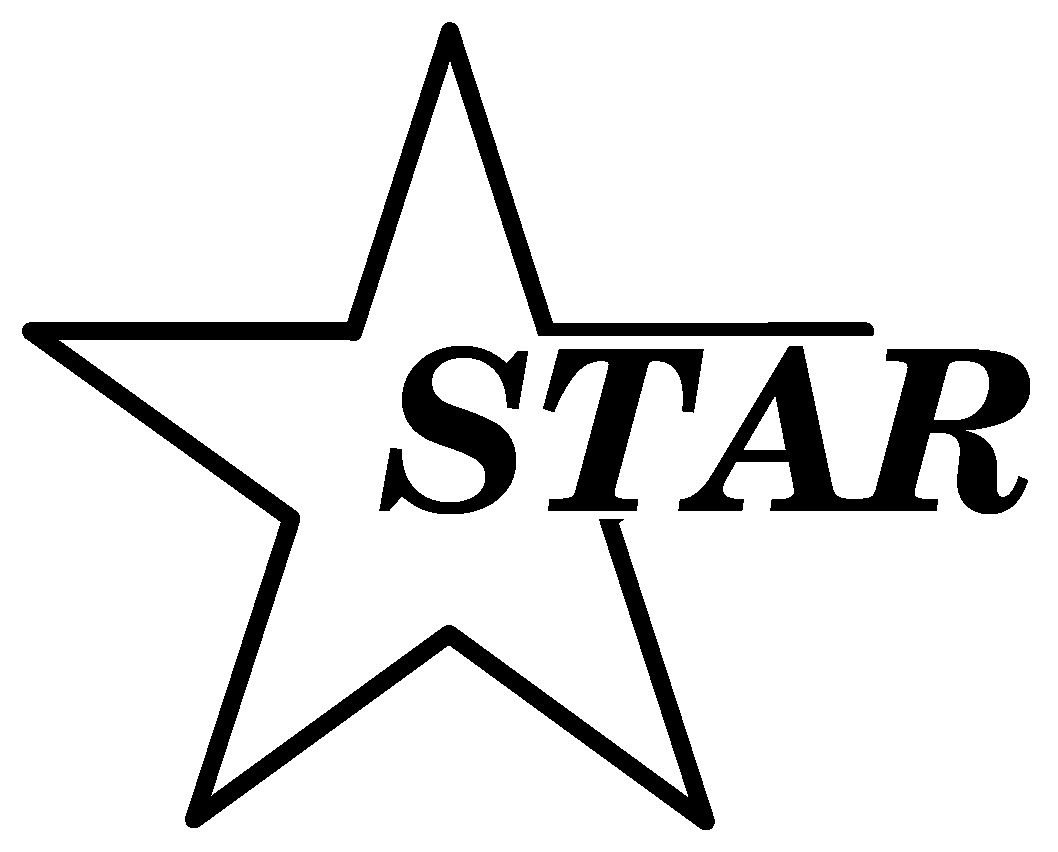
\includegraphics[width=2cm]{StarIcon.eps}}
  {\Large\bf STAR Offline Library Long Writeup}
  \hfill\mbox{}\\[3cm]
  \mbox{\includegraphics[width=\textwidth]{StEventTitle.eps}}
  \hfill\mbox{}\\[3cm]
  {\LARGE User Guide and Reference Manual \\[5mm] for Version 2}\\[2cm]
  {\LARGE $ $Revision: 2.73 $ $}  \\[5mm] % replaced by cvs with current revision
  {\LARGE $ $Date: 2002/04/18 23:38:30 $ $}  % replaced by cvs with current revision
  \vfill
\end{center}
\cleardoublepage
\end{titlepage}
\pagenumbering{roman}

%%%%%%%%%%%%%%%%%%%%%%%%%%%%%%%%%%%%%%%%%%%%%%%%%%%%%%%%%%%%%%%%%%%%
%
%    Table of content
%
%%%%%%%%%%%%%%%%%%%%%%%%%%%%%%%%%%%%%%%%%%%%%%%%%%%%%%%%%%%%%%%%%%%%
\tableofcontents
\cleardoublepage

%%%%%%%%%%%%%%%%%%%%%%%%%%%%%%%%%%%%%%%%%%%%%%%%%%%%%%%%%%%%%%%%%%%%
%
%    Introduction
%
%%%%%%%%%%%%%%%%%%%%%%%%%%%%%%%%%%%%%%%%%%%%%%%%%%%%%%%%%%%%%%%%%%%%
\pagenumbering{arabic}

\section{Introduction} %%%%%%%%%%%%%%%%%%%%%%%%%%%%%%%%%%%%%%%%%%%%%

This document contains the User Guide and Reference Manual for
\StEvent\ version 2. Like the new version of \StEvent\ this
documentation is a complete rewrite and supersedes all documentation
with revision number 1.xx. All code and documentation for the new
version has a cvs version number of greater or equal 2.00.

In this document more emphasis is put on the User Guide while the
Reference Manual part is kept shorter in terms of description of
usage.  As \StEvent\ changes this document will change accordingly and
you should always check that the revision number of the document
matches the one in the repository.

Version 2 of \StEvent\ contains significant changes as compared to the
previous versions. Part of the changes were made to cope with the
modification of the DST format in Fall of 1999, others were made to
overcome shortcomings in the previous implementation. This version is
also more flexible in terms of extendibility to allow future track and
vertex models to be incorporated easily.  The current implementation
is also meant to be used further upstream of the analysis, i.e. in the
reconstruction phase.  As a consequence the model itself became
slightly more complex in terms of navigation and structuring.

In order to explain the model in practical terms many diagrams and
plots were included in this document. Some of them show class diagrams
using the Unified Modelling Language UML. A brief introduction to UML
is given in Appendix~\ref{sec:introUML}.\index{UML}
\begin{figure}[hb]
    \begin{center}
        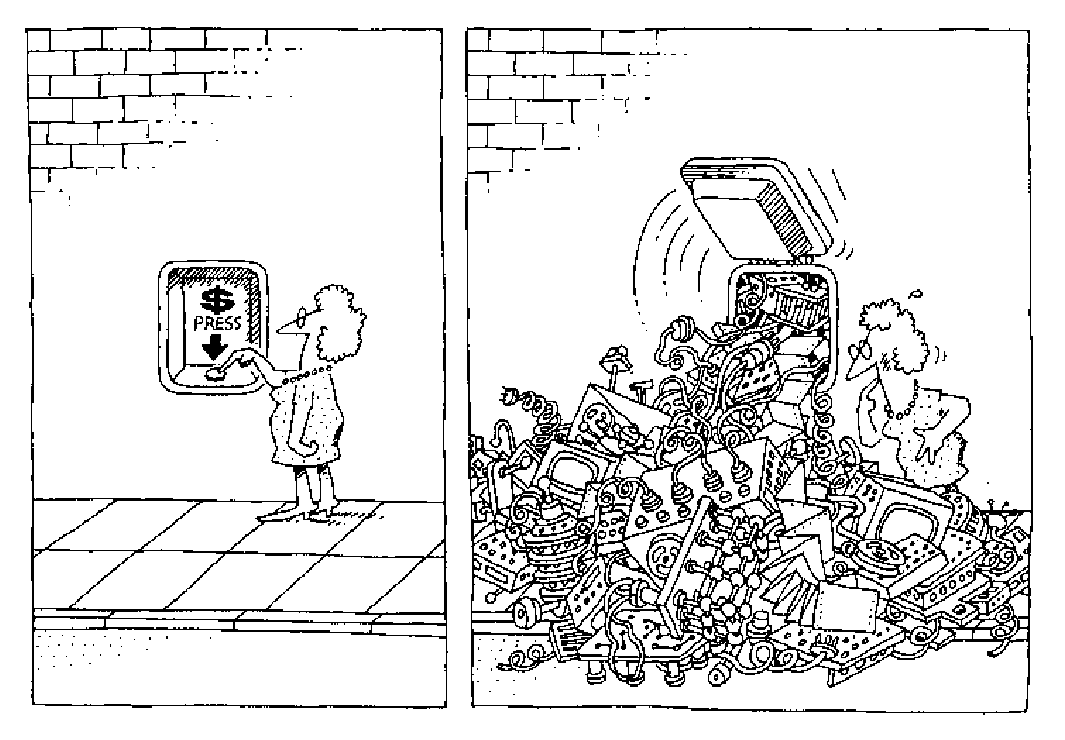
\includegraphics[width=0.9\textwidth]{cartoon1.eps}
        \caption{The task of the software development team is to
            engineer the illusion of simplicity.}
    \end{center}
\end{figure}

\clearpage

%%%%%%%%%%%%%%%%%%%%%%%%%%%%%%%%%%%%%%%%%%%%%%%%%%%%%%%%%%%%%%%%%%%%
%
%    User Guide
%
%%%%%%%%%%%%%%%%%%%%%%%%%%%%%%%%%%%%%%%%%%%%%%%%%%%%%%%%%%%%%%%%%%%%
\part{User Guide}
\clearpage

\section{Basics} %%%%%%%%%%%%%%%%%%%%%%%%%%%%%%%%%%%%%%%%%%%%%%%%%%%
\label{sec:Basics}

\subsection{Header Files}
\label{sec:HeaderFiles}
\index{header files} \index{StEventTypes.h file}

The amount of header files included in the \StEvent\ classes was
minimized to decrease dependencies between the various classes and
where ever possible forward declarations were used.  This is
especially true for the \texttt{StEvent} class itself and it is
therefore \emph{not} sufficient to include \texttt{StEvent.h} only.
Many more header files would have to be included. This is very good
for the developers since turnaround times are minimized but obviously
bad for the users for it would be very cumbersome to each time figure
out which header files one might need and which not. Therefore are
\emph{all} header files which are needed to use every little bit of
\StEvent\ contained in one single header file named
\texttt{StEventTypes.h}.  The disadvantage of this approach is that
every time one \StEvent\ class changes you have to recompile all your
code, even if the changed class is not used. This, however, should not
happen too often and it by far more convenient to deal with on header
file only.

To summarize: All you need when using \StEvent\ is to include
\texttt{StEventTypes.h} and you are all set.

\subsection{Enumerations and Constants}
\label{sec:Enumerations}
\index{enumerations} \index{constants} \index{StDetectorId.h file}
\index{StVertexId.h file} \index{StEnumerations.h file}

\StEvent\ uses a lot of enumerations for all types of purposes. This
is much more type-safe then using simple integer numbers and makes the
code more readable. All enumerations used in \StEvent\ are defined in
\texttt{StEnumerations.h}.  For users convenience some non-\StEvent\
header files as \texttt{StDetectorId.h}, \texttt{StVertexId.h} and
\texttt{StTrackMethod.h} are also included therein.
\begin{figure}[htb]
    \begin{center}
        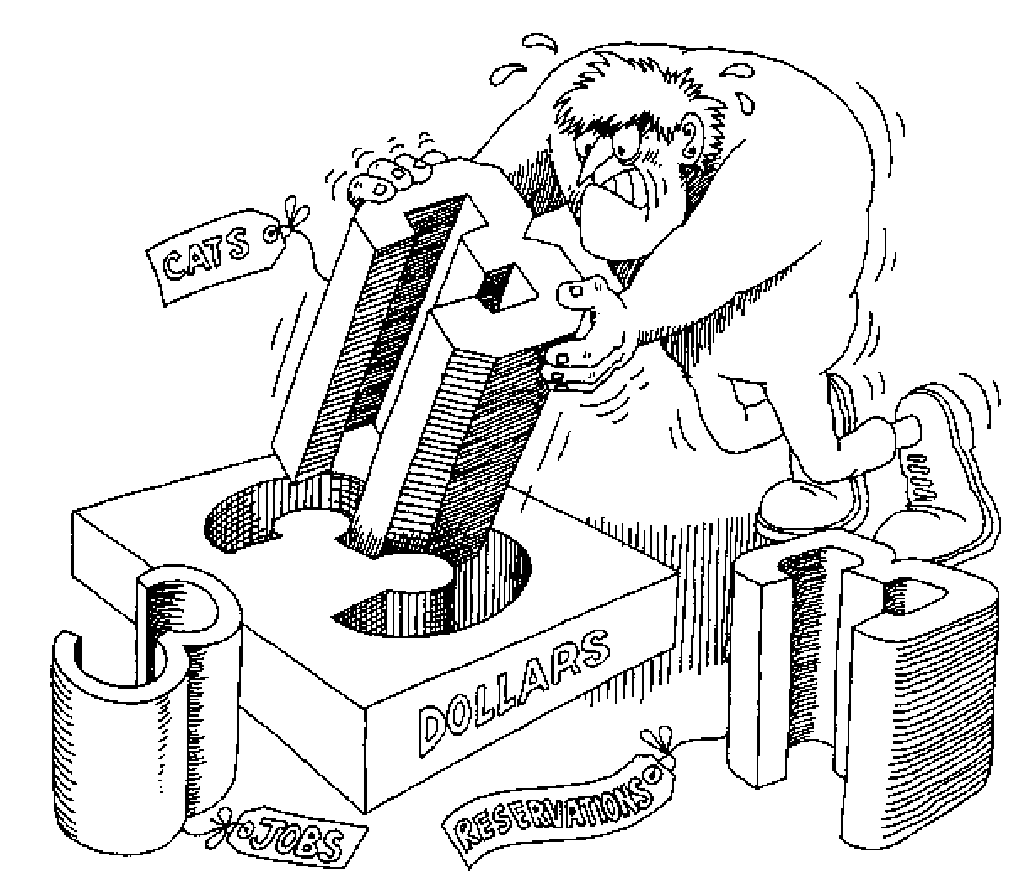
\includegraphics[width=0.45\textheight]{cartoon2.eps}
        \caption{Strong typing avoids mixing abstractions.}
    \end{center}
\end{figure}
To remind you of the names and save you the time to look them up up
every you need one they are all listed below:

\begin{verbatim}
enum StBeamDirection        {east = 0
                             yellow = 0,
                             west = 1,
                             blue = 1};

enum StBeamPolarizationAxis {transverse, longitudinal};

enum StChargeSign           {negative, positive};

enum StTrackType            {global, primary, tpt, secondary};

enum StTrackModel           {helixModel, kalmanModel};

enum StDetectorId           {kUnknownId,
                             kTpcId,
                             kSvtId,
                             kRichId,
                             kFtpcWestId,
                             kFtpcEastId,
                             kTofId,
                             kCtbId,
                             kSsdId,
                             kBarrelEmcTowerId,
                             kBarrelEmcPreShowerId,
                             kBarrelSmdEtaStripId,
                             kBarrelSmdPhiStripId,
                             kEndcapEmcTowerId,
                             kEndcapEmcPreShowerId,
                             kEndcapSmdEtaStripId,
                             kEndcapSmdPhiStripId,
                             kZdcWestId,
                             kZdcEastId,
                             kMwpcWestId,
                             kMwpcEastId,
                             kTpcSsdId,
                             kTpcSvtId,
                             kTpcSsdSvtId,
                             kSsdSvtId};

enum StVertexId             {kUndefinedVtxId,
                             kEventVtxId,
                             kV0VtxId,
                             kXiVtxId,
                             kKinkVtxId,
                             kOtherVtxId};

enum StDedxMethod           {kUndefinedMethodId,
                             kTruncatedMeanId,
                             kEnsembleTruncatedMeanId,
                             kLikelihoodFitId,
                             kWeightedTruncatedMeanId,
                             kOtherMethodId};
           
enum StTrackFittingMethod   {kUndefinedFitterId,
                             kHelix2StepId,
                             kHelix3DId,
                             kKalmanFitId,
                             kLine2StepId,
                             kLine3DId
                             kL3FitId};

enum StTrackFinderMethod    {svtGrouper,
                             svtStk,
                             svtOther,
                             tpcStandard,
                             tpcOther,
                             ftpcConformal,
                             ftpcCurrent,
                             svtTpcSvm,
                             svtTpcEst,
                             svtTpcPattern,
                             l3Standard};

enum StRichPidFlag          {eNoMip,
                             eFastEnough,
                             eLightOnPadPlane};

enum StRichHitFlag          {eDeconvoluted=1,
                             eMip=2,
                             eSaturatedPad=4 ,
                             ePhotoElectron=8,
                             eMultiplyAssignedToRing=16,
                             eAssociatedMip=32,
                             e1SigmaPi=64,
                             e2SigmaPi=128,
                             eInConstantAreaPi=256,
                             eInAreaPi=512,
                             eAssignedToRingPi=1024,
                             e1SigmaK=2048,
                             e2SigmaK=4096,
                             eInConstantAreaK=8192,
                             eInAreaK=16384,
                             eAssignedToRingK=32768,
                             e1Sigmap=65536,
                             e2Sigmap=131072,
                             eInConstantAreap=262144,
                             eInAreap=524288,
                             eAssignedToRingp=1048576};

enum StPwg                  {generic,
                             ebye,
                             hbt,
                             highpt,
                             pcoll,
                             spectra,
                             spin,
                             strangeness};
\end{verbatim}

Note that often the enumeration type names (e.g. \texttt{StTrackType})
are used as argument types. The strong C++ type checking rules ensures
the proper use of the enumeration constants already during
compilation.

Another important set of constants should be mentioned here as well,
namely the physical constants defined in \texttt{PhysicalConstants.h}.
There are too many to be listed here but you should make yourself
familiar with what constants are available. You will find the header
file in the \name{StarClassLibrary} (see Sec.~\ref{sec:furtherDoc}).
\index{StarClassLibrary} In order to define the units of the various
physical constants another set of constants defined in
\texttt{SystemOfUnits.h} is used (also from \name{StarClassLibrary}).
The latter is described in section \ref{sec:units}.

\subsection{Conventions}
\index{conventions}
\label{sec:conventions}

\subsubsection{Numbering Scheme}
\label{sec:conventionsNumbering}

All numbering follows \emph{strictly} the C/C++ convention, i.e. the
first element in an array has the index 0. This is valid for all
container, collections and lists. Here it is important to remember
that many (but not all) official STAR numbering schemes start counting
at 1.  Examples are TPC sectors and padrows, SVT barrels, layers, ladders and
wafers. Do not forget to subtract 1 when using this scheme for
addressing elements in a container.

TPC, SVT and FTPC hits return their hardware address in STAR units.
In order to select the hit container in which a hit \texttt{h} is
stored you must write:
\begin{verbatim}
evt->tpcHitCollection()->sector(h.sector()-1)->padrow(h.padrow()-1).hits();
\end{verbatim}

Many of STARs numbering schemes were defined when FORTRAN was the main
programming language and C/C++ played only a minor role. Again, the only
place where you have to deal with these conventions is when you use one of the
following methods:
\begin{itemize}
\item \texttt{StTpcHit::sector()}
\item \texttt{StTpcHit::padrow()}
\item \texttt{StFtpcHit::sector()}
\item \texttt{StFtpcHit::plane()}
\item \texttt{StSvtHit::layer()}
\item \texttt{StSvtHit::ladder()}
\item \textrm{StSvtHit::wafer(})
\item \texttt{StSvtHit::barrel()}
\item \texttt{StTrackTopologyMap::hasHitInRow(int)}
\item \texttt{StTrackTopologyMap::hasHitInSvtLayer(int)}
\end{itemize}
See the corresponding reference sections for more.

\subsubsection{References and Pointers}
\index{references} \index{pointers}

Many methods (or member functions) or \StEvent\ classes return objects
by \emph{reference} or by \emph{pointer}. This is sometimes confusing
but there is a idea behind this. Whenever an object is returned by
reference it is guaranteed to exist. No questions asked. If the object
is a container it might be empty, i.e. it has zero size, but you ask
for it you get it. Objects returned by pointer, however, are
\emph{not} guaranteed to exist. You might get a \texttt{NULL} pointer
back.  It is always a good idea to check if you really get what you
asked for.  Dereferencing a \texttt{NULL} pointer can be painful.

As you will see in the reference section many methods are provided in
two versions: a constant and a non-constant version. Don't worry about
the differences. The compiler will always choose the proper version.

\subsubsection{Units}
\label{sec:units}
\index{units} \index{system of units}

All physics quantities in \StEvent\ are stored using the official STAR
units: cm, GeV and Tesla.  Angles are given in radians\footnote{Note,
    that here \StEvent\ deviates from STAR guidelines where degrees
    are declared the official units.}  In order to maintain a coherent
system of units it is recommended to use the definitions in
\texttt{SystemOfUnits.h} from the \name{StarClassLibrary}. They allow
to 'assign' a unit to a given variable by multiplying it with a
constant named accordingly (centimeter, millimeter, kilometer, Tesla,
MeV, ...).  The constants ensure that the result after the
multiplication follows always the STAR system of units.

The following example illustrates their use:
\begin{verbatim}
double a = 10*centimeter;
double b = 4*millimeter;
double c = 1*inch;
double E1 = 130*MeV;
double E2 = .1234*GeV;

//
//   Print in STAR units
//
cout << "STAR units:" << endl;
cout << "a = " << a << " cm" << endl;
cout << "b = " << b << " cm" << endl;
cout << "c = " << c << " cm" << endl;
cout << "E1 = " << E1 << " GeV" << endl;
cout << "E2 = " << E2 << " GeV" << endl;

//
//   Print in personal units
//
cout << "\nMy units:" << endl;
cout << "a = " << a/millimeter << " mm" << endl;
cout << "b = " << b/micrometer << " um" << endl;
cout << "c = " << c/meter << " m" << endl;
cout << "E1 = " << E1/TeV << " TeV" << endl;
cout << "E2 = " << E2/keV << " keV" << endl;
\end{verbatim}
The resulting printout is:
\begin{verbatim}
STAR units:
a = 10 cm
b = 0.4 cm
c = 2.54 cm
E1 = 0.13 GeV
E2 = 0.1234 GeV

My units:
a = 100 mm
b = 4000 um
c = 0.0254 m
E1 = 0.00013 TeV
E2 = 123400 keV
\end{verbatim}
Further documentation can be found in the \name{StarClassLibrary}
manual (see Sec.~\ref{sec:furtherDoc}).\vfill

\subsection{Persistence and ROOT}
\
\label{sec:Persistence}
\index{ROOT} \index{persistence} All \StEvent\ classes inherit from
\texttt{StObject} which itself inherits from \texttt{TObject}. During
the build of \StEvent\ all classes run through \texttt{rootcint}. This
adds the following features:
\begin{enumerate}
\item All \StEvent\ classes can be used on the \texttt{root4star}
    command line.
\item Almost all \StEvent\ classes are persistent capable, i.e. they
    can be stored in ROOT files.
\end{enumerate}
As usual each coin has two sides. The disadvantage of this is that we
cannot use some features of the ANSI/ISO C++ and from the Standard C++
Library as:
\begin{itemize}
\item type bool
\item templates
\item STL containers and algorithms
\item namespaces
\end{itemize}
This however applies for the header files only. Source files are not
processed via \texttt{rootcint} and therefore all the stuff mentioned
above can be used.  And indeed in the implementation of various
\StEvent\ classes we make heavily use of the STL.
\begin{figure}[ht]
    \begin{center}
        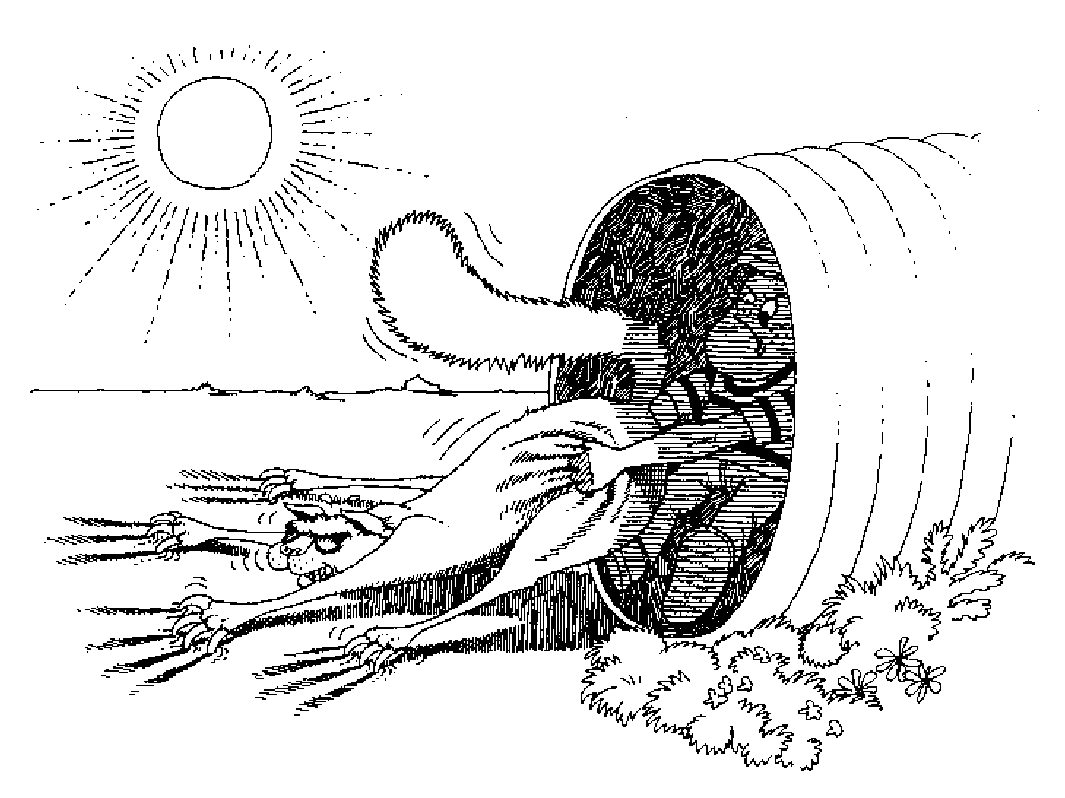
\includegraphics[width=0.5\textheight]{cartoon4.eps}
        \caption{Persistence saves the state and class of an object
            across time or space.}
    \end{center}
\end{figure}

ROOT uses typedefs for the built-in standard C++ types. This is pretty
confusing but has a good reason when it comes to persistence. This way
one can guarantee the same size (number of bytes) for the types
independent of the platform.  The ANSI/ISO standard only requires
that: \texttt{char} $\le$ \texttt{short} $\le$ \texttt{int} $\le$
\texttt{long} $\le$ \texttt{long long} and \texttt{float} $\le$
\texttt{double} $\le$ \texttt{long double}.

The types used in \StEvent\ are defined as follows:
\begin{verbatim}
typedef char           Char_t;      //Signed Character 1 byte
typedef unsigned char  UChar_t;     //Unsigned Character 1 byte
typedef short          Short_t;     //Signed Short integer 2 bytes
typedef unsigned short UShort_t;    //Unsigned Short integer 2 bytes
typedef int            Int_t;       //Signed integer 4 bytes
typedef unsigned int   UInt_t;      //Unsigned integer 4 bytes
typedef long           Long_t;      //Signed long integer 4 bytes
typedef unsigned long  ULong_t;     //Unsigned long integer 4 bytes
typedef float          Float_t;     //Float 4 bytes
typedef double         Double_t;    //Float 8 bytes
typedef unsigned char  Bool_t;      //Boolean
\end{verbatim}

Note that since April 2001 the type \texttt{long} (\texttt{Long\_t}) is not supported
by ROOT any more and cannot be used for declaration of persistent data members.

This is fine and good but there is absolutely no reason to use them in
code and function declarations.  Even worse
this can have disadvantages when it comes to calls to system functions
and speed. It also makes code less portable and readable.  Don't use
them only because you see them used in \StEvent. They are only used
for the declaration of the persistent data members.

\subsection{Container and Iterators}
\label{sec:Container}
\index{container} \index{iterators} Version 2 of \StEvent\ comes with
a new naming scheme for containers.  All containers used in \StEvent\
store objects by pointer. Technically they are all vectors and
therefore allow random-access as in
\begin{verbatim}
    pointer_to_object = container[i];
\end{verbatim}
that is they are ordered collections. There are two different types of
containers, so called structural and non-structural containers.  What
that means is rather simple. Structural containers \emph{own} the
objects they contain the others not. If you delete a structural
container all objects stored in it get deleted as well.
\begin{itemize}
\item All \textbf{s}tructural \textbf{vec}tors which store
    \textbf{p}oin\textbf{t}e\textbf{r}s carry the prefix \textbf{\texttt{StSPtrVec}}.\\
\item All other \textbf{vec}tors which store
    \textbf{p}oin\textbf{t}e\textbf{r}s carry the prefix
    \textbf{\texttt{StPtrVec}}.
\end{itemize}
That's simple. To complete the name we append the type of objects they
contain and we are done. Hence a structural container which holds
objects (or better pointer to objects) of type \texttt{StTrackNode} is
named \texttt{StSPtrVecTrackNode}. The \texttt{St} prefix of the class
is always omitted.\\
In practice it makes little difference if you are using a structural
or non-structural collection. Their interface is the same and they act
they same. The secret lies in their implementation. If you create a
container by your own you should always use the non-structural
containers. Those you can create and delete without doing \StEvent\
any harm. Never delete a structural container unless you stand with
your back to a wall and a sharp knife on your throat.

All containers used in \StEvent\ are defined in the
\texttt{StContainers.h} header file and are based on \texttt{StArray}
which was written by Victor Perevoztchikov.  \index{StContainers.h}
Currently the following containers are in use:
\begin{verbatim}
StPtrVecHit
StPtrVecTrack
StPtrVecTrackPidTraits
StSPtrVecFtpcHit
StSPtrVecKinkVertex
StSPtrVecPrimaryTrack
StSPtrVecPrimaryVertex
StSPtrVecSvtHit
StSPtrVecTpcHit
StSPtrVecTrack
StSPtrVecTrackDetectorInfo
StSPtrVecTrackNode
StSPtrVecTrackPidTraits
StSPtrVecV0Vertex
StSPtrVecXiVertex
\end{verbatim}

All containers are based on modified ROOT \index{ROOT} collections.
They allow to make \StEvent\ persistent. They good thing with
\texttt{StArray} is that all those containers offer an almost ANSI/ISO
compatible interface.  This means that \emph{both} container classes
provide the essential methods listed below. Replace \texttt{ClassName}
with any \StEvent\ class one might find in a container.
\begin{Entry}
\item[Public\\ Constructors]
    \verb+StPtrVecClassName();+\\
    \verb+StSPtrVecClassName();+\\
    Constructs an instance with zero length.

    \verb+StPtrVecClassName(unsigned int nelem);+\\
    \verb+StSPtrVecClassName(unsigned int nelem);+\\
    Constructs an instance with length \texttt{nelem}.
    
    \verb+StPtrVecClassName(const StPtrVecClassName& vec);+\\
    \verb+StSPtrVecClassName(const StSPtrVecClassName& vec);+\\
    Copy constructor. Structural containers copy also the objects they
    contain.
    
\item[Public Member\\ Functions]
    \verb+void push_back(const StClassName *pobj);+\\
    Adds object pointed to by \texttt{pobj}. If the container is not
    large enough it will automatically resize.

    \verb+unsigned int size() const;+\\
    Returns the current size of the container, i.e. the number of
    stored elements.
    
    \verb+void resize(unsigned int nelem);+\\
    Resizes the collection to size \texttt{nelem}.

    \verb+void clear();+\\
    Deletes all elements. If the container is a structural container
    all objects it holds get deleted.
    
    \verb+bool empty() const;+\\
    Checks for zero size.
    
    \verb+const StPtrVecClassNameIterator begin() const;+\\
    \verb+const StSPtrVecClassNameIterator begin() const;+\\
    Returns iterator to the the first element in the collection.
    
    \verb+const StPtrVecClassNameIterator end() const;+\\
    \verb+const StSPtrVecClassNameIterator end() const;+\\
    Returns iterator to the the last+1 element in the collection.
    
    \verb+void erase(StPtrVecClassNameIterator iter) const;+\\
    \verb+void erase(StSPtrVecClassNameIterator iter) const;+\\
    Deletes element referred to by iterator \texttt{iter}.  If applied
    to structural containers the object gets also deleted.
    
\item[Public Member\\ Operators]
    \verb+StClassName*& operator[](unsigned int i);+\\
    Returns the pointer to the \texttt{i}'th element where \texttt{i}
    runs from 0 to \texttt{size()-1}.
\end{Entry}
There are many more than one can describe here.  If you want to learn
more you better have a look at the \texttt{StArray.h} source code.

Needless to say that every container comes with two iterators, a
constant and a non-constant version.  The name of each iterator is
composed of the name of the container and the
suffix \texttt{Iterator} or \texttt{ConstIterator}.\\
Example: For the structural container \texttt{StSPtrVecTrackNode} the
iterators \texttt{StSPtrVecTrackNodeIterator} and
\texttt{StSPtrVecTrackNodeConstIterator} are defined. Iterators care
if they iterate over structural or non-structural containers so there
are different iterators for \texttt{StSPtrVecTrackNode} and
\texttt{StPtrVecTrackNode} containers.

We already mentioned that all containers are ordered vectors, hence
the two methods to iterator/loop over a collection work both as well.
It's a matter of taste which one you choose, although the iterator
version has some advantages and is somewhat safer.

\begin{verbatim}
StPtrVecTrack container;
float x;

\\ method 1
for (unsigned int i=0; i<container.size(); i++)
      x = container[i]->length();

\\ method 2
for (StPtrVecTrackIterator i = container.begin(); i != container.end(); i++)
      x = (*i)->length();
\end{verbatim}

A warning at the end. Although \texttt{StArray} provides a interface
compatible with the Standard C++ Library (former STL) it is not
guaranteed that the standard algorithms will work (\texttt{sort},
\texttt{accumulate}, \texttt{copy}, \texttt{find}, ...). You better
check this from case to case. Don't say you haven't been warned.

For your own analysis (or reconstruction) code you might use the
standard STL containers together with \StEvent\ provided that you
classes are not processed via \texttt{rootcint}. Since STL containers
are transient they are more efficient if speed and use less memory if
this is your concern.

\subsection{Getting StEvent: The StEventMaker}
\label{sec:StEventMaker}
\index{StEventMaker}

\StEvent\ is set up and filled in a ``maker'' with the name
\texttt{StEventMaker}.  This maker reads DST tables stored in memory
and does all the things to make \StEvent\ nice and useful. How the DST
gets into memory is another story and is explained in the next section
(\ref{sec:doEvents}).  In principle all you have to do is to make sure
that \texttt{StEventMaker} is in the chain and called at the right
place and at the right time.  The only public data member and the two
methods you should be aware of are:
\begin{Entry}
    
\item[Public Data\\ Member]
    \verb+bool  doLoadTpcHits;+\\
    Controls if TPC hits should be loaded (default=kTRUE).
    
    \verb+bool  doLoadFtpcHits;+\\
    Controls if FTPC hits should be loaded (default=kTRUE).
    
    \verb+bool  doLoadSvtHits; +\\
    Controls if SVT hits should be loaded (default=kTRUE).
                              
    \verb+bool  doLoadTptTracks;+\\
    Controls if TPT tracks should be loaded (default=kFALSE).
    
    \verb+bool  doPrintEventInfo;+\\
    Print or do not print info on the current \StEvent\ event.
    (default=kFALSE).  This produces a lot of output. Every major
    class is dumped, the sizes of all collections, and the first
    element in every container. Don't use it for production.
    
    \verb+bool  doPrintMemoryInfo;+\\
    Switch on/off checks on memory usage of \StEvent\
    (default=kFALSE).  In order to get a memory snapshot we use
    \texttt{StMemoryInfo} from the \name{StarClassLibrary}.  A
    snapshot is taken before and after the setup of \StEvent.  The
    numbers in brackets refer to the difference. Not available on SUN
    Solaris yet.
    
    \verb+bool  doPrintCpuInfo;+\\
    Switch on/off CPU usage (default=kFALSE). Tells you how long it
    took to setup \StEvent. Timing is performed using \texttt{StTimer}
    from the \name{StarClassLibrary}.
    
\item[Public Member\\ Functions]
    \verb+StEvent*  event();+\\
    Returns a pointer to the current \texttt{StEvent} object.
\end{Entry}

And don't forget to check if you got a \texttt{NULL} pointer. If
something went wrong this might be the case. Something else should be
mentioned here: Do \emph{not} delete the \texttt{StEvent} object you
get through these method.  It wl be
automatically deleted by the system once you read-in a new event.
\vfill

\subsection{A Standard Example: doEvents.C and StAnalysisMaker}
\label{sec:doEvents}
\index{doEvents.C} \index{StEventMaker} \index{StAnalysisMaker}
\index{root4star} \index{ROOT files} \index{XDF files}

In order to get started it is always a good idea to study a simple
example which shows the essential steps on how to analyse data using
\StEvent.  The procedure starting from scratch to run the provided
\StEvent\ usage example is
\begin{verbatim}
    stardev
    mkdir workdir
    cd workdir
    root4star
\end{verbatim}
At the root4star prompt type:
\begin{verbatim}
    .x doEvents.C(1,"-","<DST File>")
\end{verbatim}
where \texttt{<DST File>} must be replaced by an actual DST file. Ask
one of your colleges where to find the latest DST files in either XDF
(extension .xdf) or ROOT (extension .root) format.

This will run the \texttt{\$STAR/StRoot/macros/analysis/doEvents.C}
macro which runs a chain consisting of two makers:
\begin{description}
\item[\texttt{StEventMaker}:] Read events from DST input files (XDF
    files or ROOT files; the file is handled appropriately based on
    file type) and load \StEvent.
\item[\texttt{StAnalysisMaker}:] Picks up the \StEvent\ event and
    analyze it (incorporates a few simple examples).
\end{description}
It runs the chain on either a single file or all files under a
specified root directory (see doEvents.C for details). Example
invocations are:

Processes 10 events from the specified XDF file.\\
\hspace{1cm}\verb+.x doEvents.C(10,"-","/some_directory/some_dst_file.xdf");+\\

Processes 42 events from the specified ROOT file.\\
\hspace{1cm}\verb+.x doEvents.C(42,"-","/some_directory/some_dst_file.root");+\\

Processes all events from all files found recursively under the
specified directory.\\
\verb+.x doEvents.C(9999,"/some_directory/"," ");+\\

The multiple-files feature works for XDF and ROOT files.  To play with
it yourself you can pick up \name{StAnalysisMaker} and modify it piece
by piece or use it as a template for a Maker of your own that works
with \StEvent:

\begin{verbatim}
    mkdir StRoot/StMyAnalysisMaker
    cp $STAR/StRoot/StAnalysisMaker/* StRoot/StMyAnalysisMaker/
    [edit and modify]
    cons +StMyAnalysisMaker
    cp $STAR/StRoot/macros/analysis/doEvents.C ./
    [edit to use your maker]
    root4star
\end{verbatim}
At the ROOT prompt type
\begin{verbatim}
    .x doEvents.C(<your arguments>);
\end{verbatim}
By the time you gain more experience your ``maker'' will become more
and more sophisticated but the basic idea shown in the example stays
the same.

\subsection{Further Documentation}
\label{sec:furtherDoc}
\index{documentation}

In STAR all documentation specific to a packages is under cvs control
and stored in the same repository as the source code of the package.
You will find it usually in a directory called \texttt{doc}.  In
addition to that every package should contain a \texttt{README} and a
\texttt{index.html} file with further information. (Note the
``should''.)

\StEvent\ makes use of various classes from the
\name{StarClassLibrary} (SCL).  Examples are \texttt{StThreeVector},
\texttt{StHelix} and \texttt{StParticleDefinition}. You should have a
version of the SCL manual at hand. It also contains a description of
the helix track model used in STAR and contains many
examples.\index{SCL} \index{StarClassLibrary}

Very important is also the documentation from the
\texttt{\$STAR/pams/global/idl} area. Here you will find a detailed
description of the DST tables content.  Since StEvent pretty much
reflects this content (although in a different way and approach) this
is the place to check if you don't understand the meaning of certain
variables or methods.  In this manual we cannot go too much into
detail. It's already thick enough.

And finally, you really should have the C++ bible from B.~Stroustrup
within 100 feet distance from your desk. The more you get into C++ and
OO the more you will appreciate this book. We already mentioned that
\StEvent\ is a bit complex and especially when you look deeper into
its internal structure you will find weird things like virtual
constructors, overloaded new/delete operators and much more.  Then it
is nice to have Bjarnes book.  \index{Stroustrup, Bjarne} \clearpage


\section{The StEvent Model} %%%%%%%%%%%%%%%%%%%%%%%%%%%%%%%%%%%%%%%%

In the following we describe the basic concepts of \StEvent.  This is
not to describe every class and every method in detail but to explain
the idea behind it and illustrate a few things in simple examples.  If
you need more details have a look at the reference section and if you
want to know \emph{everything} about \StEvent\ you have to visit the
source code directly.

\subsection{Event Header}
\index{event header} \index{event summary} \index{StEvent}
\index{StEventSummary}

The event header carries the same name as the whole package:
\texttt{StEvent}. Confused?  Don't worry, when we talk about the
package we write \StEvent, when we talk about the class we write
\texttt{StEvent}.\\
The class \texttt{StEvent} plays a special role since it is the entry
point and the upper most object of the whole \StEvent\ tree. From here
you
can reach every single bit and byte there is on the DST.\\
Obviously, this makes the \texttt{StEvent} class somewhat ``fat''.
Figure ref{fig:umlEvent} shows only a very
small fraction of the class design around \texttt{StEvent}.
\begin{figure}[htb]
    \begin{center}
        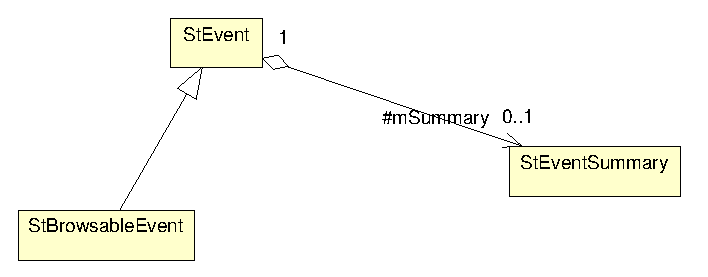
\includegraphics{event.eps}
        \caption{Class diagrams for \texttt{StEvent} and
            \texttt{StEventSummary}.}
        \label{fig:umlEvent}
    \end{center}
\end{figure}
The class \texttt{StEventSummary} contains lots of information
gathered during the reconstruction of the event like: the total number
of tracks, the number of positive or negative tracks, the number of
vertices of certain types, and several \emph{quasi}-histograms which
hold for example transverse momenta distributions and other important
quantities. 
Check the pointer to the event summary before you use it. It could be
\texttt{NULL}.
 
As already mentioned \texttt{StEvent} opens the door to all the info
there is on the DST.  In order to get there you have to navigate
through the tree. Only few objects, mostly container and collections,
can be reached directly from the \texttt{StEvent} objects.  Here's a
list of some important objects which are directly stored in
\texttt{StEvent} and let you climb further down the tree:
\begin{enumerate}
\item Collection of software monitors
\item TPC hit collection
\item FTPC hit collection
\item SVT hit collection
\item List of all track nodes
\item List of the detector info for each track
\item Primary vertices (mostly only one)
\item List of all V0 vertex candidates
\item List of all Xi vertex candidates
\item List of all kink vertex candidates
\item Level-0 trigger
\end{enumerate}
And remember, an object you get \emph{by pointer} is not guaranteed to
exist, an object you get \emph{by reference} always exist.

What else does \texttt{StEvent} contain? Well, all the usual stuff one
would expect to see in an event header: event identifier, time when
the event was recorded, the trigger mask, the bunch crossing number
and more. For a complete reference see section \ref{sec:StEvent}.

\subsection{Software Monitors}
\index{software monitors}

The STAR DST contains a bunch of tables called software monitors.
Before we go into details let's clarify what this is. During the
reconstruction of the various detectors lots of statistics and summary
information is generated which is not necessarily of importance for
the physics of the event but tells you a lot on how the reconstruction
programs performed. These are mostly quantities which cannot be
derived from other objects in \StEvent\ and would be lost otherwise.
In a sense they \emph{monitor} the reconstruction details.
That's where the name 'software monitor' comes from.\\
\begin{figure}[hbt]
    \begin{center}
        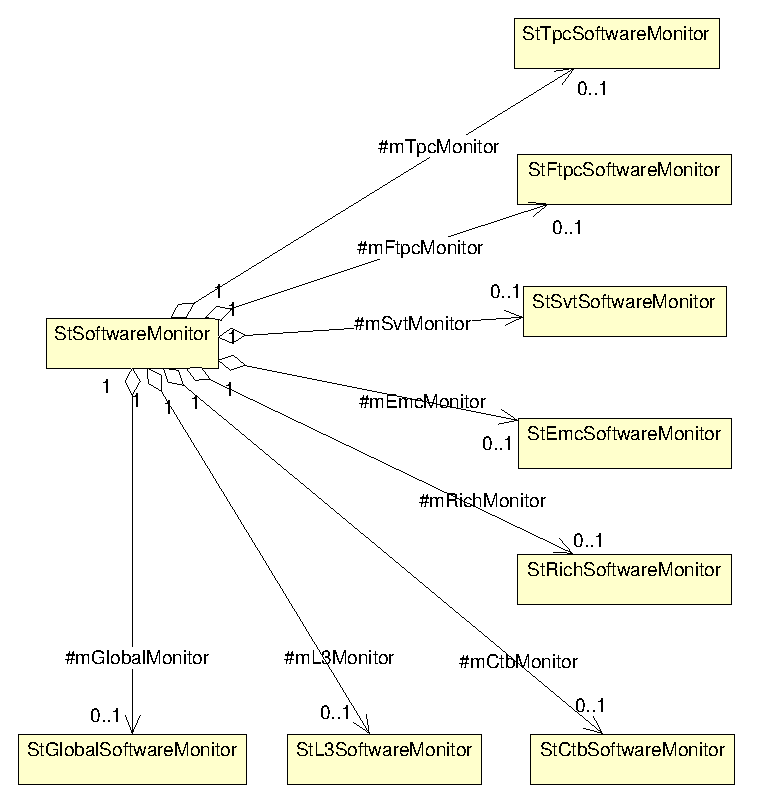
\includegraphics{monitors.eps}
        \caption{Class diagrams for the software monitors.}
        \label{fig:umlMonitors}
    \end{center}
\end{figure}

There are many of these monitors and even the ``global''
reconstruction has one. This is not really a detector but a large
fraction of our software deals with combining all the detectors in
order to create global tracks and find the primary vertices.

Since there are many they have to be organised in a transparent way.
This is depicted in Fig.~\ref{fig:umlMonitors} where all monitor
classes and their relations are shown.  You get the actual instance of
\texttt{StSoftwareMonitor} from \texttt{StEvent} and then you can
select which component, i.e.~which monitor object you want by invoking
the proper method. These methods are named after the component they
return: \texttt{tpc()} returns a pointer to the
\texttt{StTpcSoftwareMonitor}, \texttt{svt()} to the
\texttt{StSvtSoftwareMonitor} -- well, you get the idea. As usual you
should check for \texttt{NULL} pointers. If a detector was not
reconstructed in the reconstruction chain it's likely that you will
not find the corresponding monitor.

The specific software monitor classes are pretty simple flat classes.
They have no relation with any other class. All they do is to hold
data. Because of this, they have no member access functions and all
data members are public. In order to make things easier for people
moving from table-based analysis to \StEvent-based analysis we kept
even the table names.  With other words the software monitor classes
match their table counterparts 1:1.  The names are not always
descriptive but the author got tired of inventing new names.  You'll
find more details on what is what in the reference section of this
manual.

Here a simple example on how to use the software monitors:
\begin{verbatim}
void printTpcClusterInfo(ostream& os = cout, StEvent* event)
{
    StTpcSofwareMonitor *tpcMon = 0;

    if (event && event->softwareMonitor())
        tpcMon = event->softwareMonitor()->tpc();


    if (!tpcMon) return;       // no monitor

    os << "Total # of TPC cluster:" << tpcMon->n_clus_tpc_tot;
    for (int i=0; i<24; i++) {
        os << "Inner sector " << i << " has "
           << tpcMon->n_clus_tpc_in[i] << " cluster" << endl;
        os << "Outer sector " << i << " has "
           << tpcMon->n_clus_tpc_out[i] << " cluster" << endl;
    }
}
\end{verbatim}
Note that, as everywhere in \StEvent\ indices run from \texttt{0} to
\texttt{size-1}.  If you are new to C/C++ and wonder why this is so,
you really should read section \ref{sec:conventionsNumbering}.\vfill

\subsection{Trigger and Trigger Detectors}
\index{trigger} \index{detectors}

The \textbf{trigger} is put together from data recorded by a bunch of
trigger detectors combined in some logic. So far STAR deals with 4
trigger levels numbered 0 -- 3.  Currently only level-0 (L0) is
implemented. Others will follow.  All trigger classes inherit from a
common base class \texttt{StTrigger}.  As mentioned above, at the
moment there is only one derived class \texttt{StL0Trigger} as
depicted in Fig.~\ref{fig:umlTrigger}.
\begin{figure}[htb]
    \begin{center}
        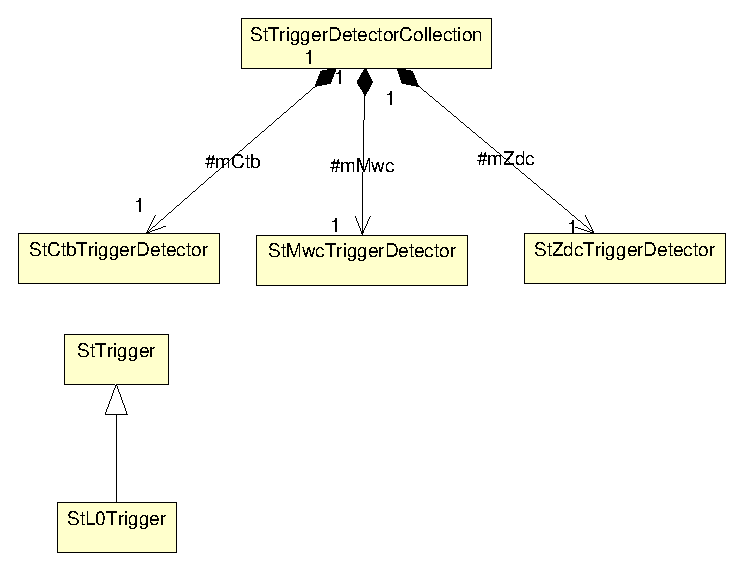
\includegraphics{trigger.eps}
        \caption{Class diagrams for the trigger detector collection and
            the \texttt{StTrigger} hierarchy.}
        \label{fig:umlTrigger}
    \end{center}
\end{figure}
The class contains everything there is available about the actual
trigger: trigger word, trigger action word, multiplicities, and more.
The trigger is directly contained in the \texttt{StEvent} class. In
order to get a pointer to the L0 trigger use:
\texttt{StEvent::l0Trigger()}. Even if we repeat us here: it is a
pointer and therefore can be \texttt{NULL}. At the moment all
simulations have no trigger data. You were warned.

The \textbf{trigger detectors} are those detectors which data is used
in the trigger (which doesn't mean that the data isn't useful for
other things as well). There's a couple of them: the Central Trigger
Barrel (CTB), the Zero Degree Calorimeter (ADC), the Vertex Position
Detector (VPD), and the Multiwire Proportional Chamber (MWC). This
means we need a collection to hold them together and indeed this is
what \texttt{StTriggerDetectorCollection} is all about. The trigger
detector design is shown in Fig.~\ref{fig:umlTrigger}.  The collection
holds all classes which describe the different trigger detectors:
\texttt{StMwcTriggerDetector}, \texttt{StCtbTriggerDetector},
\texttt{StZdcTriggerDetector}, and \texttt{StVpdTriggerDetector} (not
shown).  These trigger detectors store the actual ADC and TDC values
including some calculated quantities. Check in the reference section
for more details.  The collection is a member of \texttt{StEvent}. To
get a pointer to the collection use:
\texttt{StEvent::triggerDetectorCollection()}. From there you get the
specific trigger detectors through a set of methods.  The methods are
named after the component they return by reference: \texttt{ctb()}
returns a reference to the \texttt{StCtbTriggerDetector},
\texttt{mwc()} to the \texttt{StMwcTriggerDetector}, and so on.  Since
they are returned by reference you can be sure the objects exist. No
checks necessary. Note that ``exist'' is not a synonym for ``makes
sense''. The reason for this is that the DST contains the data for all
trigger detectors in one big table. If it available the collection
(StTriggerDetectorCollection) is created else
\texttt{StEvent::triggerDetectorCollection()} will return
\texttt{NULL}.  Once created the data in the table is used to setup
the instances of the various trigger detectors. If a specific detector
wasn't used its data is set 0 (so the author hopes) but the data is
still there.

Here's an example which dumps the CTB data in form of a table:
\begin{verbatim}
void dumpCtb(StEvent* event)
{
    if (!(event && event->triggerDetectorCollection())) return;

    StCtbTriggerDetector &ctb = event->triggerDetectorCollection()->ctb();

    cout << " tray | slot |    mips    |      time   \n";
    cout << "----------------------------------------\n";

    for (int i=0; i<ctb.numberOfTrays(); i++) 
        for (int j=0; j<ctb.numberOfSlats(); j++) 
            cout << setw(5) << i <<   " | "
                 << setw(4) << j <<   " | "
                 << setw(10) << ctb.mips(i, j, 0) << " | "
                 << ctb.time(i, j, 0) << endl;


    cout << "\nL0 trigger:\n";
    if (event->l0Trigger()) {
        PR(event->l0Trigger()->mwcCtbMultiplicity());
        PR(event->l0Trigger()->mwcCtbDipole());
        PR(event->l0Trigger()->mwcCtbTopology());
        PR(event->l0Trigger()->mwcCtbMoment());
    }
    else
        cout << "not available" << endl;
}
\end{verbatim}
Again, we are using the \texttt{PR()} macro from \texttt{StGlobals.hh}
to save some typing. The names of the methods speak for themself.

\subsection{Tracks}
\index{tracks}

This is probably the most complex part of the design.  Before we get
into too much detail we give a brief introduction on what a track is
and explain the differences between \emph{global} and \emph{primary}
tracks. We then introduce the track \emph{node} which plays a very
central role in the \StEvent\ track model.  The different pieces of
information which make a track such as the track geometry and the
various traits are explained later together with a short introduction
to filters, which, as you will learn, allow to apply predefined
algorithm to select and filter information out of the data.

\subsubsection{Introduction to Tracks}
\index{primary tracks} \index{global tracks}

The STAR tracker, known as \texttt{tpt}, performs the tracking in the
main STAR tracking detector the TPC. It finds a set of hits, which
\texttt{tpt} assume to belong to one track and applies fits in order
to determine the track parameters. Once this is done the track is
passed along the chain.  Points from other detectors might be added.
At the end this track is then fitted with a more sophisticated fitting
method and from there on is called a \textbf{global} track (class
\texttt{StGlobalTrack}).  The name "global" stems from the fact that
this is a fit which is possibly composed of his from several tracking
detectors.

But wait, this is not the end of the story. STAR can do better than
this. By using all global tracks we can reconstruct the primary vertex
(or vertices) with pretty good accuracy. A track which originates from
the primary vertex (and most do) can be refitted using the primary
vertex as additional point.  This increase dramatically the accuracy
in which STAR can measure particles, both in terms of direction and
momentum.  If a global track points back close enough to the primary
vertex and the refitting works out well (whatever that means) then
this track, or better the refitted track, becomes a \textbf{primary}
track (class \texttt{StPrimaryTrack}). A primary track only makes
sense if it refers to a primary vertex.  If a primary track is found
the global track which was used to create it makes almost no sense any
more and could be dropped, \texttt{if} you trust the procedure.
However, things aren't as perfect and the primary track might have
been misidentified.  For that reason STAR keeps currently all global
tracks. That means that for every primary track there is one
corresponding global track but every global track does not necessarily
have a corresponding primary track. The fit might have failed badly.
In future this might change and we might be able to drop
a fraction of the global tracks if the primary track is superior. \\
If a primary track fit succeeds the new track parameters and its
errors are stored.  To really confuse you, we should mention that even
the number of hits might change, since the newly refitted track might
exclude some hits and/or add new hits.  \StEvent\ is able to cope with
all these scenarios and that is one of the reasons why version 2 is
somewhat more complex than good old version 1.

So far so good. But what's with the tracks which fail the fit.
Obviously these aren't primary tracks and -- you guessed it -- come
from a secondary vertex.  Here, things become a bit difficult. While a
primary vertex can be found easily secondary vertices are more tricky
to detect (at least in a Heavy-Ion collision) and can hardly be
identified unambiguously. If one could do so, one could repeat the
same trick as with the primary tracks and refit the global track using
the secondary vertex such making it a secondary track. But we can't --
at least for now. As as consequence STAR doesn't use the concept of
secondary tracks yet.

All global and primary tracks are fitted according to a certain
tracking model. Some models include the effect of energy loss and
multiple scattering in the fit and the fit parameters therefore
depends on the mass of the particle which created the track. This is
not know a priori or at least cannot be determined unambiguously. In
this case the same track might be fitted with different mass
hypothesis.  This not only alters the fit parameters and errors but
possibly also the hits assigned to the track.  In a sense these are
tracks created from the same \texttt{seed}. How we keep track of all
these different flavours is explained in the next section.

To summarize: STAR has two kinds of tracks global tracks which can
come from wherever they want and primary tracks which always point
back to the primary vertex. The position of the primary vertex was
used to refit the primary tracks.

\subsubsection{The Concept of the Track Node}
\label{sec:node}
\index{track node}

As we have seen in the previous section there are two kinds of tracks
(global and primary) of which each might get possibly fitted with
different models or algorithms such creating a whole bunch of tracks.
But we have to keep in mind that all come originally from the same
\texttt{seed} formed early in the reconstruction chain. Only one of
them can be the true track, or better only one comes closest to the
truth. If we count tracks we can only count all of them as one.  Many
students spent by far too much time hunting the problem of
double-counting.\\
\begin{figure}[htb]
    \begin{center}
        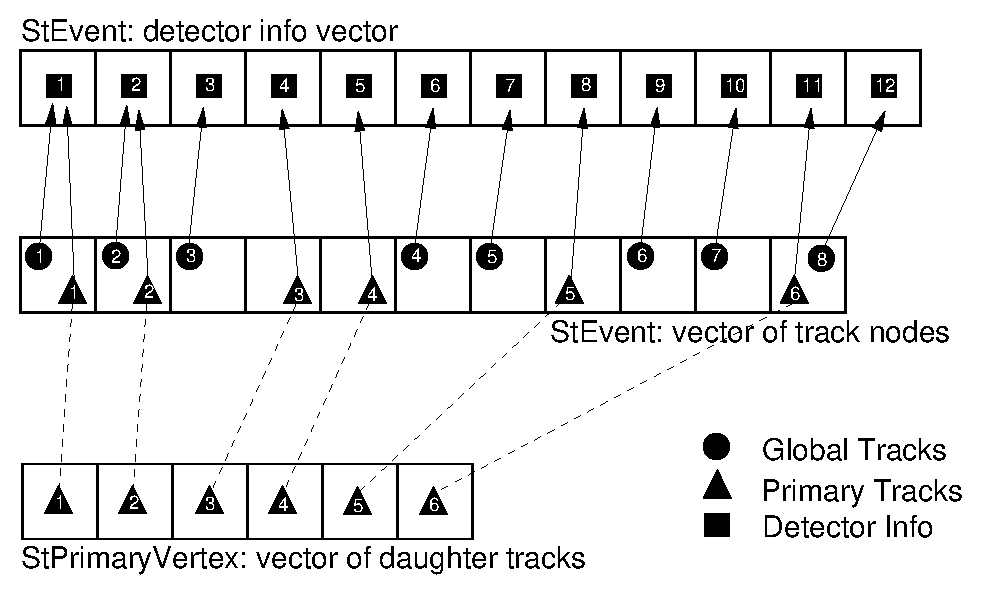
\includegraphics[width=\textwidth]{nodes.eps}
        \caption{Schematic view of the track node collection and
            its relation to the detector info collection and the list
            of daughter tracks of the primary vertex.}
        \label{fig:nodes}
    \end{center}
\end{figure}
We have to have a way to tell that all these ``flavours'' belong
together, even if they have different fit parameters or even a
slightly different set of hits. This is were the track \textbf{node}
comes into the game (class \texttt{StTrackNode}).

A track node holds all tracks which originate from the same seed.
Every track knows about the node it belongs to and thus allows to
navigate from one track in the node to the other.  Each node contains
1--n tracks. This is depicted in Fig.~\ref{fig:nodes}.  The array
shown in the middle of the picture shows the collection of nodes as
held by the StEvent class itself. Every element (depicted as a box)
represents one node which contains a primary (solid triangle) and/or a
global track (solid circle). The length of the track node list lies
between: max(N$_{primary}$, N$_{global}$) and N$_{primary}$ +
N$_{global}$.

\subsubsection{Detector Information}
\label{sec:detInfo}
From the previous section you probably got the impression that a given
primary track and its referring global track share lots of
information.  Actually, there is much less to share then one might
think.  Almost everything changes or can change when a track is
refitted. One of the few things which often do not change are the hits
used in the tracks.  If the global track fit points back to the vertex
the additional constraint, i.e.~the position of the primary
vertex, changes the parameters in fact only slightly. \\
If the set of hits, or the detector information, is the same then it
belongs in a separate class so one can use it for all tracks in the
same node.  This is why there is a class \texttt{StTrackDetectorInfo}.
 
All detector specific information (essentially the list of hits) is
contained in this class.  A track can well live without them since all
the reconstruction is already done.  And indeed on the long term STAR
cannot afford to write \emph{all} hits to DST. In this case each track
might or might not have a pointer to an existing instance of
\texttt{StTrackDetectorInfo}.  Since several tracks can share this
instance it is obvious that no track can own them. This is why all
objects of type \texttt{StTrackDetectorInfo} are stored in a separate,
flat and simple list which is directly accessible from
\texttt{StEvent}. Each track only points to its detector info. This is
depicted in Fig.~\ref{fig:nodes}.  The upper array represents a
possible list of detector info objects.  As you can see tracks in a
node mostly share the same detector info but this doesn't need to be
the case. If a primary vertex fitter decides to reject one or more
hits and/or adds new hits than the detector infos might be different
although the tracks are in the same node (see right most node in the
figure as an example). It makes obviously no sense to keep both tracks
in the same node if the hits are \emph{very} different but if only one
or two hits are different they still are related - somewhat.

Note, that the size of the detector-info list is larger or equal the
number of nodes.

\subsubsection{The Track Classes}

So far we only discussed the basic concepts. It is time now to have a
closer look at the design of specific classes. It is really helpful to
look at the class diagrams in Fig.~\ref{fig:umlTracks}. It looks
complicated but once you get the idea things become easy.

The base class \texttt{StTrack} is an abstract class, i.e. you won't
be able to create an instance of it. The two concrete classes are
\texttt{StGlobalTrack} and \texttt{StPrimaryTrack}.  Both have the
\textbf{same} interface as \texttt{StTrack}. Whatever you can do with
an instance of \texttt{StGlobalTrack} you can do with
\texttt{StPrimaryTrack} as well. The difference is in the
implementation but not in the interface. For this very reason whenever
a track is returned by a method or is used as an argument, a pointer
or a references to \texttt{StTrack*} is used. This is were
polymorphism comes in handy.

\begin{figure}[p]
    \begin{center}
        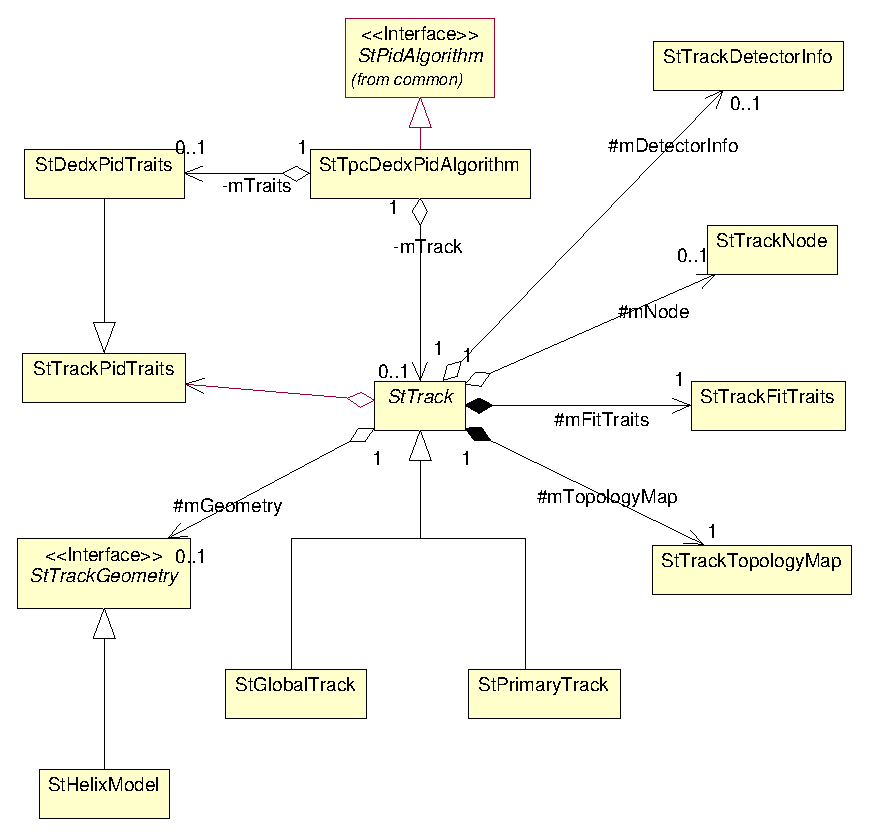
\includegraphics{tracks.eps}
        \caption{Class diagrams for \texttt{StGlobalTrack} and
            \texttt{StPrimaryTrack} including related classes
            and dependencies.}
        \label{fig:umlTracks}
    \end{center}
\end{figure}
With other words it is sufficient to explain \texttt{StTrack} and the
other two come for free. As you can see in Fig.~\ref{fig:umlTracks}
\texttt{StTrack} is composed of several classes. It either contains
them by value or by pointer. There are:
\begin{description}
\item[StTrackGeometry] \index{StTrackGeometry} This is an abstract
    class which only serves as an interface the the actual, concrete
    implementation. You get a pointer to the instance via the
    \texttt{StTrack::geometry()} method. The track geometry contains
    exactly what the name implies.  It describes the parameters of the
    track which let us describe the path of the particle in the
    detector. Which set of parameters are actually obtained from a fit
    depends strongly on the track model.  However, we don't want any
    new track model to make you change your code and this exactly is
    the \textit{reason d'etre} for \texttt{StTrackGeometry}. It
    defines the interface and with it the parameters it has to
    provide. If the track model does not directly use or produce them
    they have to be derived. This insures that every tracking model
    which gets plugged in doesn't break anything. The class guarantees
    that you always get:
    \begin{itemize}
    \item curvature (in cm$^{-1}$)
    \item charge (in units of +e)
    \item dip angle (in radians)
    \item psi (in radians) , i.e.~$\psi$ not $\phi_0$ -- watch
        out\footnote{if you don't know the difference have a look in
            the appendix of the \name{StarClassLibrary} manual.  There
            the parameters are explained in detail.}
    \item origin (as a \texttt{StThreeVectorF})
    \item momentum at the origin (as a \texttt{StThreeVectorF})
    \item a helix (as a \texttt{StPhysicalHelixD})
    \end{itemize}
    The helix now is somewhat special since it obviously implies that
    the track can be described as such. Although this is not always
    true (FTPC, low momentum tracks in TPC) it is a very good
    approximation for almost all TPC tracks -- and a helix can be
    handled analytically. This makes it very useful to find the
    distance-of-closest approach to a given point, to extrapolate the
    path of the track and to easily get the 3-momentum at every point
    along the trajectory.
    
    At the moment there is actually only one concrete class
    implemented and that is -- you guessed it -- the helix model
    (\texttt{StHelixModel}). This is where all the calculations (if
    any) are done to make sure you get what you ask for.
    
    If you want to know which model is actually used you may call the
    \texttt{StTrackGeometry::model()} method which returns an element
    of the enumeration type \texttt{StTrackModel}. See in section
    \ref{sec:Enumerations} what types are available or check directly
    in \texttt{StEnumerations.h}.
    
\item[StTrackFitTraits] \index{StTrackFitTraits} Every track gets
    fitted and every fit algorithm provides errors, a covariant matrix
    and a $\chi^2$ value -- if the algorithm is worth a penny.  This
    and a bit more is stored in the \texttt{StTrackFitTraits} which
    you get through \texttt{StTrack::fitTraits()} by reference! By
    reference since \texttt{StTrack} contains the instance by value.
    It is always present. No need to check for \texttt{NULL} pointer
    and such crap. There's no need for an abstract
    layer hence we don't need a pointer.\\
    There might be different ways to fit and different ways to
    calculate the errors but they better be available, always. After
    all, this is what determines the quality of the track and thus
    decides if tracks get included in the analysis or get rejected.
    
\item[StTrackNode] \index{StTrackNode} See section \ref{sec:node}.
    \texttt{StTrack::node()} will return a pointer to the node the
    track belongs to.
    
\item[StDetectorInfo] \index{StDetectorInfo} See section
    \ref{sec:detInfo}.  \texttt{StTrack::detectorInfo()} will return a
    pointer to its respective detector info. Note, that there is no
    way to navigate back from the detector info to the tracks which
    are using it.
    
\item[StPidTraits] \index{StPidTraits} Each track has a list
    (container) of so called PID traits. Each of them contains
    information on the ID of the particle. What they actual provide is
    not specified. All we know is that we get an object which tells us
    something about the identity of the track.  \texttt{StPidTraits}
    is an abstract class. The concrete classes are
    \texttt{StDedxPidTraits}, \texttt{StRichPidTraits}, and
    \texttt{StTofPidTraits}. The latter two are not implemented yet.
    This part is a bit complicated and that's why it got its own
    section (see \ref{sec:pidTraits} below).
    
\item[StTrackTopologyMap] \index{StTrackTopologyMap} The STAR
    detectors produces all together almost a million hits. In order to
    keep the DST size at a moderate level all cannot get stored,
    probably none on the long term. There are however many reasons to
    keep a minimum level of information about the hits used to fit the
    tracks. This minimum level is contained in
    \texttt{StTrackTopologyMap}. For more check out the reference
    manual.
    
\end{description}

\subsubsection{TPT Tracks}
\label{sec:tptTracks} \index{TPT tracks}
You probably never will need them but they are mentioned here for completeness.
The main reason they are in StEvent is for debugging purposes and studies by reconstruction
experts. For physics always use global or primary tracks. 

The current STAR tracker for the TPC is called TPT. It not only finds the tracks
but also performs some simple fits. In a sense 'TPT tracks' are real tracks, but,
and this is important, TPC only tracks. In addition the track parameters are determined
in a very simplistic fitting method. \\
TPT tracks are described by \texttt{StTptTrack} which is identical in look and feel to
\texttt{StGlobalTrack}. Tracks of this type are owned by the referring track node.
And this is almost everything there is to say about them.

\subsubsection{PID Traits}
\label{sec:pidTraits}
PID traits contain information about the identity of the track. Every
detector will supply some sort of information useful for PID and there
will be several methods for each detector to derive the same kind of
information. The most basic ways to find out about the PID of a track
are:
\begin{description}
\item[dE/dx] in TPC, FTPC and SVT.
\item[Ring area densities] in the RICH detector.
\item[TOF] information from the TOF patch.
\item[Topology info] where the ID of a track can be derived, or at
    least be constraint, from its measured decay products (e.g.
    kinks).
\end{description}
It seems natural that, as the experiment progresses, STARs PID methods
will be refined and new algorithms will get developed. If every PID
method for every detector would require an concrete interface (via
concrete classes) the class \texttt{StTrack} would be subject to
permanent modifications. Schema evolution would become daily business.
Very bad.  The only way out of this dilemma is to shield
\texttt{StTrack} from this kind of PID inflation by adding
an abstract layer. And this is all what \texttt{StTrackPidTraits} is for.\\
\texttt{StTrack} now holds only a list of pointers to
\texttt{StTrackPidTraits} and doesn't need to know about any specific
details. Since the various ways of doing PID differ quite
significantly there is hardly any data member or method they have in
common.  That's why the abstract class \texttt{StTrackPidTraits} has
only one member which returns the ID of the detector the PID info
originates from.  The PID traits collection in \texttt{StTrack}
obviously contains concrete objects which will provide the data you
are looking for but \texttt{StTrack} is screened from any further details. \\
There is currently only one concrete class implemented which is meant
to contain the dE/dx derived from various methods in the TPC, FTPC and
SVT: \texttt{StDedxPidTraits}. If a specific PID method or detector
needs more than this class provides a new one has to be created. For
sure, a new class is needed for the RICH, for the TOF and for
topology-PID.  But that's something
for the future.\\
The class \texttt{StDedxPidTraits} gives you the mean dE/dx, the error
on the mean, the number of points used, and the method which was applied to
calculate it.  This method is returned as an enumeration
(\texttt{StDedxMethod}) and can take the following values:
\texttt{kTruncatedMeanId}, \texttt{kEnsembleTruncatedMeanId},
\texttt{kLikelihoodFitId}, \texttt{kWeightedTruncatedMeanId}, and
\texttt{kOtherMethodId}. The latter is a place-holder which can be
used for tests and code development (see also
sec.~\ref{sec:Enumerations}).

So now I have a list of \texttt{StTrackPidTraits} with which I hardly
can do anything -- how do I get the object I need? Good questions with
an easy answer. You have to scan the list and pick out the object you
are looking for and \textbf{cast} it up to the concrete class for only
the concrete class will reveal its content.  This is where you
obviously need RTTI (Real Time Type Information) as provided by
ANSI/C++. Alternatively you can use ROOT-RTTI which we will not
discuss here.  And here an example to show how it works:
\begin{verbatim}
//
// Given a pointer 'track' to a valid track object
// we first get the list.
//
StSPtrVecTrackPidTraits& traits = track->pidTraits()

//
// What we want here is the dE/dx from the TPC from
// a simple truncated mean. This means:
// 1. detector = kTpcId
// 2. class    = StDedxPidTraits
// 3. method   = kTruncatedMeanId
//
StDedxPidTraits* pid;        // this is what we want

for (int i=0; i<traits.size(); i++) {
     if (traits[i]->detector() == kTpcId) {
         // Here we know it is some PID object derived from TPC data

         // Now the dynamic cast
         pid = dynamic_cast<StDedxPidTraits*>(traits[i]);

         // If traits[i] is NOT of type StDedxPidTraits the dynamic cast
         // returns a NULL pointer. No other cast can do this !!!
         // If we succeed we found the right object.
         if (pid && pid->method() == kTruncatedMeanId) break;
     }
}

if (pid) {
   // We found what we wanted  ....
   cout << pid->mean() << endl;
}
\end{verbatim}
\begin{figure}[htb]
    \begin{center}
        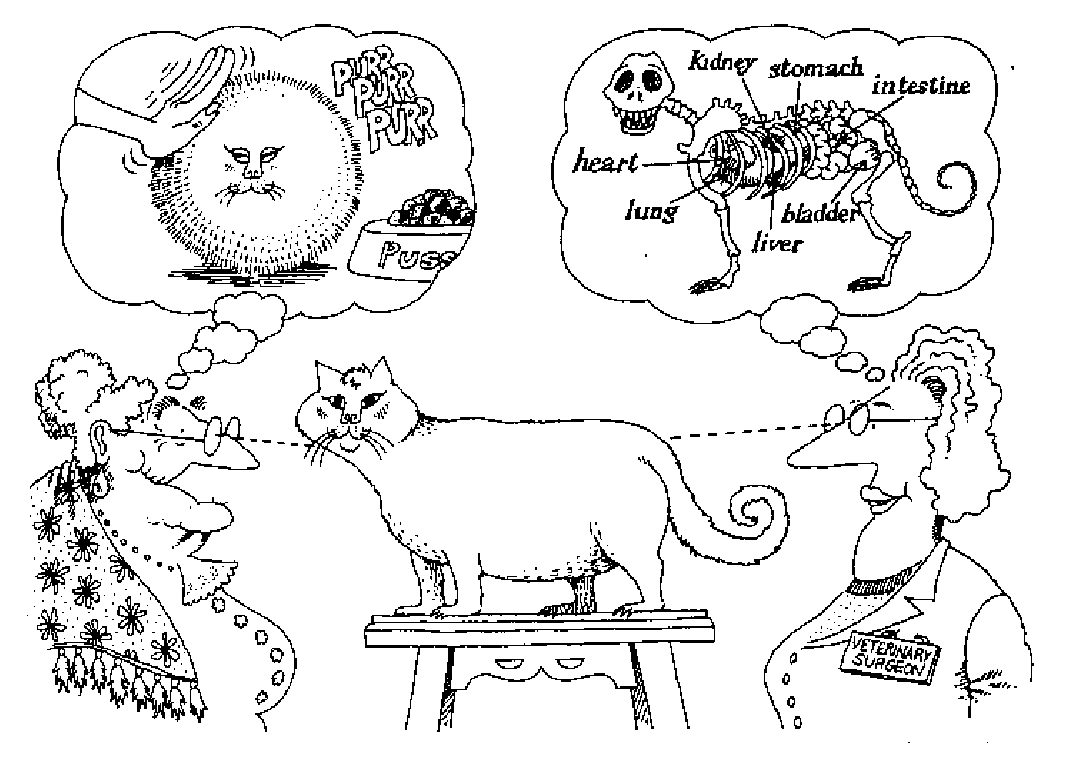
\includegraphics[width=0.7\textwidth]{cartoon5.eps}
        \caption{Abstraction focuses upon the essential characteristic
            of some object, relative to the perspective of the
            viewer.}
    \end{center}
\end{figure}
Instead of a \texttt{dynamic\_cast} one also could use
\texttt{typeid()} as in
\begin{verbatim}
        if (typeid(*pid) == typeid(StDedxPidTraits))
           pid = static_cast<StDedxPidTraits*>(traits[i]);
\end{verbatim}
which is probably even faster.

In the example we used \texttt{StTrack::pidTraits()} to get the whole
list. In fact we can do better.  Since we already know we want PID
from the TPC we can use the overloaded version
\texttt{StTrack::pidTraits(StDetectorId)} to get all PID traits for
one specific detector.  What happens internally is that the method
scans the whole list, creates a new container and puts in all the
objects (or better the pointer to the objects) with PID data from a
the requested detector. This is what the method returns.

Now we save a line and the example above looks like:
\begin{verbatim}
StPtrVecTrackPidTraits traits = track->pidTraits(kTpcId);
StDedxPidTraits* pid;

for (int i=0; i<traits.size(); i++) {
    pid = dynamic_cast<StDedxPidTraits*>(traits[i]);
    if (pid && pid->method() == kTruncatedMeanId) break;
}

if (pid) {
   // We found what we wanted  ....
   cout << pid->mean() << endl;
}
\end{verbatim}

But that's not the end of it. We can do even better, but this is
described in the next section (\ref{sec:pidAlgorithm}) since it needs
a bit more explanation. With what was shown here you already get very
far. Remember that every cast but a \texttt{dynamic\_cast} will cause
you nothing but trouble. Have a look at your favourite introductory
C++ textbook on \texttt{dynamic\_cast} and RTTI.  (If your favourite
introductory C++ textbook doesn't discuss \texttt{dynamic\_cast},
carefully tear out all pages and recycle them.  Dispose of the book's
cover in an environmentally sound manner, then borrow or buy a better
textbook.)

\subsubsection{PID Algorithm, Filters and Functors}
\label{sec:pidAlgorithm}
\index{PID algorithm} \index{filter} \index{functor}
\index{StPidAlgorithm and examples} In OO one often talks about
\emph{functors} which are essentially nothing but functions wrapped in
a class. The reason why one wants to do this are manifold. One is that
one can build up a hierarchy of functions by inheritance and, this is
even more important, lifetime control. A function is gone when it
finishes while an object still lives happily in memory. Thus a functor
can do some work and then rest until someone comes and picks up the
information it has stored.  Also it is \emph{much} easier to pass
objects than pointer to functions. (Ever tried to pass an array of
function pointers in C ?).

If a functor is used to scan a list and returns only a subset of the
elements it is called a filter. In the context of PID traits we use a
PID algorithm which serves as a filter but is supposed to do a bit
more than this.

The essential method all tracks provide is:
\begin{verbatim}
const StParticleDefinition*
StTrack::pidTraits(StPidAlgorithm& algo) const;
\end{verbatim}

As usual \texttt{StPidAlgorithm} is an abstract class (functor) which
does nothing but defining the interface to the ``real'' function,
i.e.~ it defines the arguments it takes and what it has to return.
\texttt{pidTraits()} then calls this function, passing to it the
proper arguments. The important thing is that we require
\texttt{pidTraits()} to return 'something', namely the definition of
the most probable particle (for \texttt{StParticleDefinition} see the
\name{StarClassLibrary}). How it does that is up to the guy who
implements the concrete
functor, that is you.\\
The decleration of \texttt{StPidAlgorithm} from
\texttt{StFunctional.h} looks as follows:
\begin{verbatim}
struct StPidAlgorithm
{
    virtual StParticleDefinition*
    operator() (const StTrack&, const StSPtrVecTrackPidTraits&) = 0;
}
\end{verbatim}
\index{StParticleDefinition} The function which does the work is
invoked when the operator() is invoked.  All the data needed to do the
job are passed as arguments.  This is the track itself and the list of
all PID traits. The PID algorithm now can pick up the detector (or
detectors) and methods of its choice and derive the final answer. With
other words the algorithm is doing the PID.  Over time you will
collect a set of PID algorithms which you can plug in whenever needed.
They may use different detectors and methods or possibly combine them.

To make it completely clear, here's an example of a PID algorithm
which uses the dE/dx of the TPC and the SVT and returns the most
probable particle:
\begin{verbatim}
// MyPID.h
#include "StEventTypes.h"
struct MyPID : public StPidAlgorithm
{
    StParticleDefinition*
    operator() (const StTrack&, const StSPtrVecTrackPidTraits&);
};

// MyPID.cxx
#include "MyPID.h"
StParticleDefinition*
MyPID::operator() (const StTrack& track,
                   const StSPtrVecTrackPidTraits& traits)
{
   StDedxPidTraits* tpcPid = 0;
   StDedxPidTraits* svtPid = 0;

   for (int i=0; i<traits.size(); i++) {
        StDedxPidTraits *pid = dynamic_cast<StDedxPidTraits*>(traits[i]);
        if (pid && pid->method() == kTruncatedMeanId) {
           if (pid->detector == kTpcId)
               tpcPid = pid;
           else if (pid->detector == kSvtId)
               svtPid = pid;
        }
   }

   if (svtPid && tpcPid) {
       // do something with the numbers and figure
       // out what particle is most likely
       // ....

       // Assume it's a pion
       if (track.geometry()->charge() > 0)
           return StPionPlus.instance();
       else
           return StPionMinus.instance();
   }
   else
      return 0;
}
\end{verbatim}
The piece of code where you make use of the class might look as this:
\begin{verbatim}
#include "MyPID.h"
// ....

MyPID mypid;
const StParticleDefinition *part = track->pidTraits(mypid);
cout << "The name of the particle is " << part->name() << endl;
cout << "its mass is m = " << part->mass() << " GeV/c2" << endl;
\end{verbatim}

So far so good, but what if I don't want to return something, what if
I simply want to have a look without making a decision? Easy, return a
\texttt{NULL} pointer -- who cares.  As long as you know what the
algorithm is doing this should work fine.

Here's a simple version of this approach. Let's say we are interested
in TPC dE/dx (truncated mean) and nothing else:
\begin{verbatim}
// MyTpcAlgo.h
#include "StEventTypes.h"
class MyTpcAlgo : public StPidAlgorithm
{
public:
    MyTpcAlgo() {mTraits = 0;}

    StParticleDefinition*
    operator() (const StTrack&, const StSPtrVecTrackPidTraits&);

    StDedxPidTraits* traits() { return mTraits; }

private:
    StDedxPidTraits *mTraits;
};

// MyTpcAlgo.cxx
#include "MyTpcAlgo.h"
StParticleDefinition*
MyTpcAlgo::operator() (const StTrack& t, const StSPtrVecTrackPidTraits& traits)
{
   mTraits = 0;
   for (int i=0; i<traits.size(); i++) {
        if (traits[i]->detector() != kTpcId) continue;
        StDedxPidTraits *pid = dynamic_cast<StDedxPidTraits*>(traits[i]);
        if (pid && pid->method() == kTruncatedMeanId) {
           mTraits = pid;
           break;
        }
   }
   return 0;
}
\end{verbatim}

This now works really as a filter. We added three things which
\texttt{StPidAlgorithm} does not require: A private data member
\texttt{mTraits} which is meant to hold the "right" type of PID traits
we want to filter out, a method to return it \texttt{traits()}, and a
constructor to initialize the private data member to \texttt{NULL}.
Note, that the base class \texttt{StPidAlgorithm} only wants us to
define the \texttt{operator()}, the rest is up to us. We are free to
add whatever we want.

This is how it can be used:
\begin{verbatim}
#include "MyTpcAlgo.h"
// ....

MyTpcAlgo tpcDedx;
track->pidTraits(tpcDedx);

cout << tpcDedx.traits()->mean() << endl;
cout << tpcDedx.traits()->errorOnMean() << endl;
\end{verbatim}

This code uses very few lines. The code in \texttt{MyTpcAlgo} is
highly re-usable and whoever uses the PID algorithm saves a lot of
typing.

\index{StTpcDedxPidAlgorithm} In \StEvent\ there is actually one
concrete PID algorithm implemented: \texttt{StTpcDedxPidAlgorithm}.
The algorithm used stems from Craig Ogilvie.  It filters out the TPC
dE/dx object (StDedxPidTraits) and returns the most probable particle,
but also keeps all the information selected. The additional methods
now make use of the stored information and let you work with the
object after the select/filter operation is done. It is much more
complicated then the examples shown here but the basic idea is the
same. See \ref{sec:StTpcDedxPidAlgorithm} for details.

\subsection{Vertices}
\label{sec:vertices}
\index{vertices} \index{StVertex} \index{StMeasuredPoint}
\index{StPrimaryVertex} \index{StV0Vertex} \index{StXiVertex}
\index{StKinkVertex}

A vertex is, after all, a measured point in space and that's why the
basic vertex class \texttt{StVertex} inherits from an abstract base
class called \texttt{StMeasuredPoint}. The same is actually true for
all hits.  A measured point has a position, position errors, and even
a covariant error matrix but it doesn't implement them. All it does is
to guarantee that everything which inherits from it provides these
methods. The advantage is that all measured points (i.e. hits and
vertices) have the same basic methods which is a great advantage when
it comes to fitting or drawing.

The base class for all vertices is \texttt{StVertex}. In addition to
the methods inherited from \texttt{StMeasuredPoint} each vertex
provides a \texttt{type()} method which returns an enumeration type
StVertexId (see section \ref{sec:Enumerations}), a $\chi^2$ value from
the fit, a pointer to the parent track and a list of daughter tracks.
However, \texttt{StVertex} is still abstract. The five concrete vertex
classes are:
\begin{description}
\item[\texttt{StPrimaryVertex}] to hold the events vertex (or
    vertices)
\item[\texttt{StCalibrationVertex}] to hold the various
    vertices used for calibration and test purposes.
\item[\texttt{StV0Vertex}] which is primarily used for K$_0$ and
    $\Lambda$ decay vertices
\item[\texttt{StXiVertex}] for $\Xi$ decay vertices
\item[\texttt{StKinkVertex}] for kink vertices
\end{description}
The UML diagram for the vertices classes is shown in
Fig.~\ref{fig:vertex}.

The primary vertex \texttt{StPrimaryVertex} class plays an important
role since it holds all primary tracks. This is depicted in
Fig.~\ref{fig:nodes}. If the
class gets deleted all primary tracks get deleted. \\
The primary vertex, or vertices, are directly stored in the
\texttt{StEvent} class. Usually, in Au-Au collisions there's only one
``primary'' vertex but there are cases (pile-up events) where there
can be more than one.  That's why \texttt{StEvent} has the
\texttt{numberOfPrimaryVertices()} method and the access member
function has an optional argument \texttt{primaryVertex(unsigned int
    i=0)}.  Hence \texttt{event->primaryVertex()} implies
\texttt{event->primaryVertex(0)}. If there is more than one you have
to give the index.\\
The primary vertices are ordered according to the number of daughters
(i.e.~primary tracks) they hold. The first in the list is always the
the vertex with the most daughter tracks. \index{primary vertices, order of}
\begin{figure}[htb]
    \begin{center}
        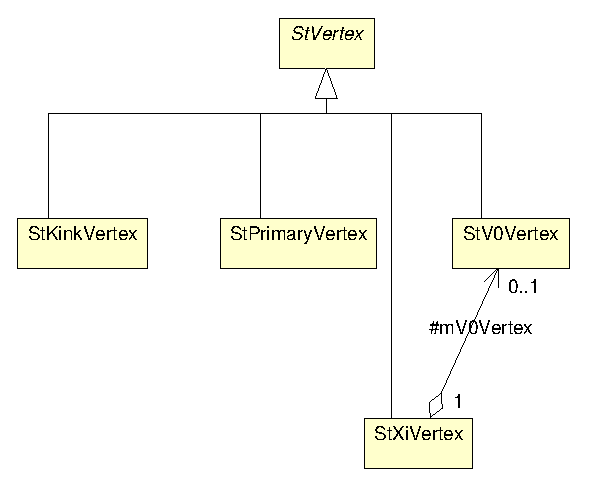
\includegraphics{vertex.eps}
        \caption{Vertex class diagrams and their dependencies.
            \texttt{StCalibrationVertex} is not shown.}
        \label{fig:vertex}
    \end{center}
\end{figure}

All secondary vertices \texttt{StV0Vertex}, \texttt{StXiVertex}, and
\texttt{StKinkVertex}, store only references to their daughter tracks
but they do not own them. In the reconstruction phase the daughter
tracks are actually refitted with the vertex constraint but do not
become StTrack objects. Only the momentum is extracted and stored as
data member in the referring vertex class. This might change later but
this is how it is done now. The referenced daughter tracks are always
global tracks (\texttt{StGlobalTrack)}.

By the way, although all vertex classes hold a parent pointer it is
(currently) always zero. This might change in future. \\
All secondary vertices are stored in flat containers and accessible
from \texttt{StEvent}. The methods to obtain a reference (!) to the
collections are \texttt{StEvent::v0Vertices()},
\texttt{StEvent::kinkVertices()}, and \texttt{StEvent::xiVertices()}.
\begin{figure}[htb]
    \begin{center}
        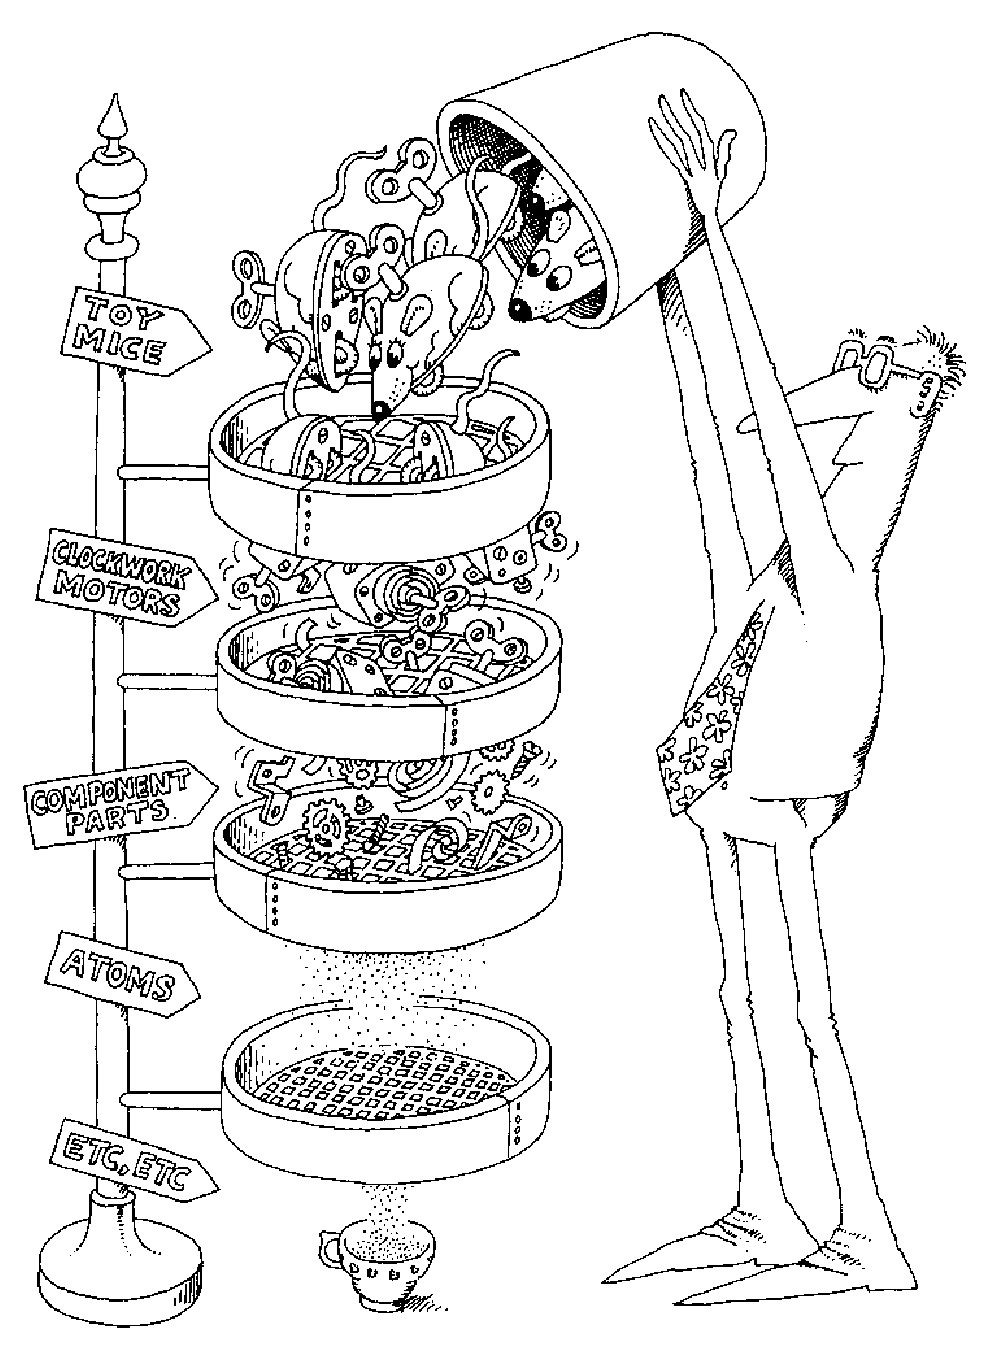
\includegraphics[height=0.7\textheight]{cartoon3.eps}
        \caption{Abstraction from a hierarchy}
    \end{center}
\end{figure}

\subsection{Hits}
\index{hits} \index{StMeasuredPoint} The base class for all concrete
hit classes is \texttt{StHit} which itself inherits from
\texttt{StMeasuredPoint}. So all the 'position' related stuff comes
with the measured point: position, position errors, and a covariant
error matrix.  \texttt{StHit} adds what all hits have in common such
as a charge, a detector ID, a track reference count, i.e. the number
of tracks which use the hit, and a method to return the list of
tracks which reference the hit.  The list of tracks is created on the
fly since a hit doesn't know anything about tracks. Only tracks hold
references to their hits.
\begin{figure}[htb]
    \begin{center}
        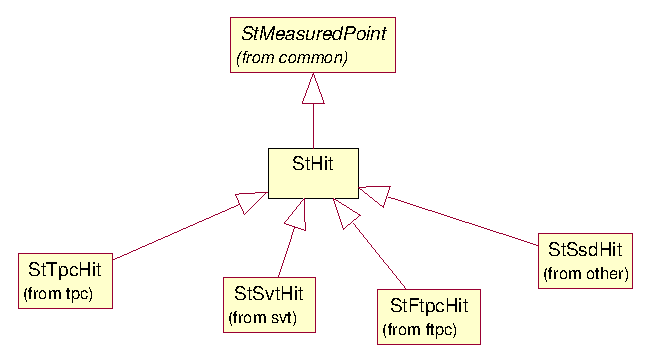
\includegraphics{hits.eps}
        \caption{The \texttt{StHit} class and its subclasses and superclasses.}
        \label{fig:hits}
    \end{center}
\end{figure}

Here an example on how to obtain a list of all global and primary
tracks which use a given hit:
\begin{verbatim}
void f(StHit& hit, StEvent& event)
{
   StPtrVecTrack gvec, pvec;
   gvec = hit.relatedTracks(event->trackNodes(), global);
   pvec = hit.relatedTracks(event->trackNodes(), primary);

   if (gvec.size() + pvec.size() != hit.trackReferenceCount())
      cerr << "This cannot happen unless something is very wrong." << endl;

   cout << "The hit is used to fit "
        << gvec.size() << " global tracks and "
        << pvec.size() << "primary tracks."

   cout << "The momenta of the tracks are:" << endl;
   int i;
   for (i=0; i<gvec.size(); i++)
       cout << gvec[i]->geometry()->momentum() << endl;
   for (i=0; i<pvec.size(); i++)
       cout << pvec[i]->geometry()->momentum() << endl;
}

\end{verbatim}

Needless to say that \texttt{StHit} is an abstract class. The concrete
classes are: \texttt{StTpcHit}, \texttt{StSvtHit}, and
\texttt{StFtpcHit}. The class diagram in Fig.~\ref{fig:hits} shows
their relation. In the following we describe the different classes in
detail.

\subsubsection{TPC hits}
\index{TPC hits} \index{TPC sectors and rows} \index{StTpcHit}
\index{sectors} \index{rows} Each hit returns its position in global
coordinates. In addition hit classes also provide information on their
\emph{local} coordinates through methods which decode a detector
specific data word. For the TPC hits there are methods to return the
sector number (1-24) and row number (1-45).  Please read section
\ref{sec:conventionsNumbering} about the difficulties with numbering
schemes starting at 1.  There are two additional member functions
\texttt{padsInHit()} and \texttt{pixelsInHit()} which return
information on the number of pads and pixels used to compose the hit.
See \ref{sec:StTpcHit} for details.
\begin{figure}[htb]
    \begin{center}
        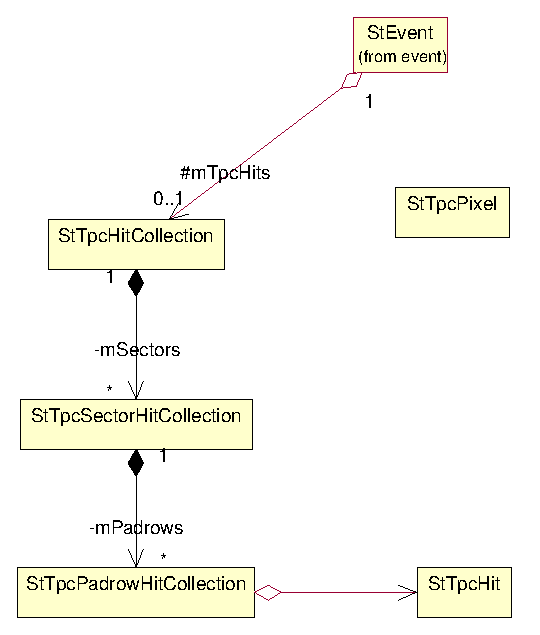
\includegraphics{tpc.eps}
        \caption{Class diagrams of the TPC hit storage scheme: sector/padrow.}
        \label{fig:tpc}
    \end{center}
\end{figure}

The hits are stored in a tree-like structure organized
according to their ``natural'' location, i.e. sector- and row-wise.
The collection you obtain (by pointer) via
\texttt{StEvent::tpcHitCollection()} holds a list of sectors
(\texttt{StTpcSectorHitCollection}) which itself holds a list of padrows
(\texttt{StTpcPadrowHitCollection}). Each padrow finally contains the list of
hits in this padrow. This is illustrated in the class diagrams in
Fig.~\ref{fig:tpc}. You get the idea when you look at the following
example:
\begin{verbatim}
const int isec = 3;    // 4th sector
const int irow = 24;   // 25th row

cout << "sector " << isec << " contains "
     << event->tpcHitCollection()->sector(isec)->numberOfHits()
     << " hits" << endl;

StSPtrVecTpcHit& theHits =
event->tpcHitCollection()->sector(isec)->padrow(irow)->hits();

cout << "sector " << isec << " padrow " << irow << " contains "
     << theHits.size() << " hits" << endl;

for (int i=0; i<theHits.size(); i++) {
    cout << theHits[i]->position() << endl;
    cout << theHits[i]->charge() << endl;
    cout << theHits[i]->padsInHit() << endl << endl;
    cout << theHits[i]->pixelsInHit() << endl << endl;
    assert(theHits[i]->padrow() == irow);
    assert(theHits[i]->sector() == isec);
}
\end{verbatim}
The top collection (\texttt{StTpcHitCollection}) and each sector 
(\texttt{StTpcSectorHitCollection}) provide a method
\texttt{numberOfHits()} which returns just that, the number of all TPC
hits and the number of hits in the corresponding sector.

This organization scheme makes it much easier to perform gain and
residual studies and can be better integrated into the reconstruction
phase than a long flat list of hits. The disadvantage is that looping
over \emph{all} hits does require somewhat more code but selecting
hits in certain rows or sectors is easy and very efficient.

\subsubsection{FTPC hits}
\index{FTPC hits}
\index{FTPC planes and sectors}
\index{StFtpcHit}
\index{sectors}
\index{planes}

The FTPC hit class \texttt{StFtpcHit} is very similar to the TPC
version.  However, because of the different detector geometry the hits
are stored according to planes (20) and then sectors (6). This is
depicted in Fig.~\ref{fig:ftpc}. Other than the TPC hit the FTPC hit
has a method to return the size of the hit in time direction
(\texttt{timebinsInHit()}) but no method to return the number of
pixels per hit. See \ref{sec:StFtpcHit} for details.  You probably
should also read the warnings in section
\ref{sec:conventionsNumbering} on the numbering schemes.

\begin{figure}[htb]
    \begin{center}
        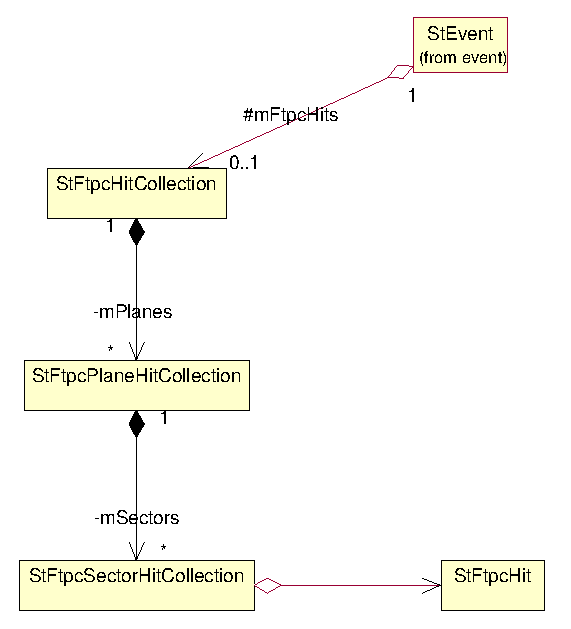
\includegraphics{ftpc.eps}
        \caption{Class diagrams of the FTPC hit storage scheme: plane/sector.}
        \label{fig:ftpc}
    \end{center}
\end{figure}
The following is the equivalent example to the one above but for the FTPC:
\begin{verbatim}
const int iplane = 11;
const int isec   = 3;

cout << "plane " << iplane << " contains "
     << event->ftpcHitCollection()->plane(iplane)->numberOfHits()
     << " hits" << endl;

StSPtrVecFtpcHit& theHits =
event->ftpcHitCollection()->plane(iplane)->sector(isec)->hits();

cout << "plane " << iplane << " sector " << isec << " contains "
     << theHits.size() << " hits" << endl;

for (int i=0; i<theHits.size(); i++) {
    cout << theHits[i]->position() << endl;
    cout << theHits[i]->charge() << endl;
    cout << theHits[i]->padsInHit() << endl << endl;
    cout << theHits[i]->timebinsInHit() << endl << endl;
    assert(theHits[i]->plane() == iplane);
    assert(theHits[i]->sector() == isec);
}
\end{verbatim}

\subsubsection{SVT hits}
\index{SVT hits} \index{StSvtHit} \index{ladder, SVT} \index{layer, SVT}
\index{wafer, SVT} \index{barrel, SVT}

The SVT consist of 3 barrels (6 layers) with up to 16 (8) ladders
each. Each ladder has up to 7 wafers. Consequently the
\texttt{StSvtHit} class provides methods to return the local
coordinates exactly in these ``units'': \texttt{barrel()} returns
1--3, \texttt{layer()} returns 1--6, \texttt{ladder()} returns 1--16,
and \texttt{wafer()} returns 1--7. If you are puzzled why these
numbers start at 1 have a look at section
\ref{sec:conventionsNumbering}.  Because of the more detailed local
coordinates there is not enough space to store any further details on
the hits as it is the case for the TPC and FTPC.  The SVT hits are
stored in a tree organized as shown in Fig.~\ref{fig:svt}.  The top
collection (\texttt{StSvtHitCollection}) contains 3 barrel
collections.  Each barrel collection
(\texttt{StSvtBarrelHitCollection}) contains up to 16 ladder
collections and each (\texttt{StSvtLadderHitCollection}) contains up
to 7 wafer collection (\texttt{StSvtWaferHitCollection}). The latter
finally contains the hits.  With other words, the hits are stored per
wafer.  Each of the shown classes provide a method
(\texttt{numberOfHits()}) to return the number of hits stored in the
referring subcomponent. 
\begin{figure}[htb]
    \begin{center}
        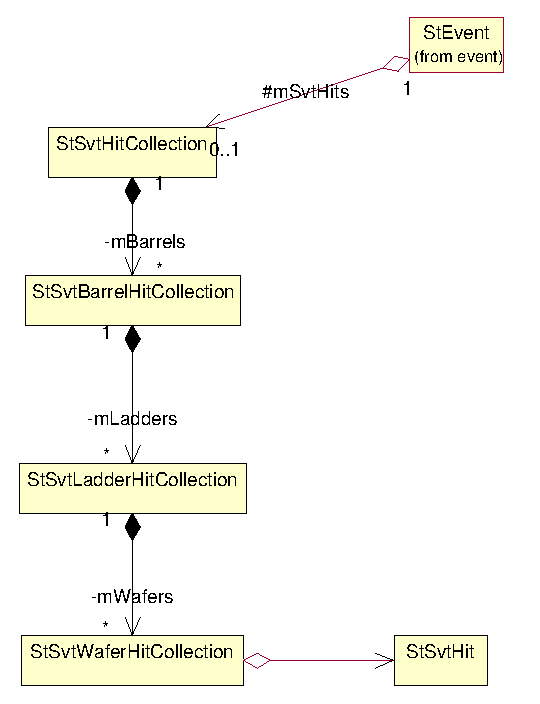
\includegraphics{svt.eps}
        \caption{Class diagrams of the SVT hit storage scheme: barrel/ladder/wafer.}
        \label{fig:svt}
    \end{center}
\end{figure}

The following is the equivalent example to the two previous ones but for the SVT hits.
The scheme is always the same:
\begin{verbatim}
const int ibarrel  = 1;  // 2nd barrel
const int iladder  = 10; // 11th ladder
const int iwafer   = 3;  // 4th layer

cout << "barrel " << ibarrel << " contains "
     << event->svtHitCollection()->barrel(ibarrel)->numberOfHits()
     << " hits" << endl;

StSPtrVecSvtHit& theHits =
event->svtHitCollection()->barrel(ibarrel)->ladder(iladder)->wafer(iwafer).hits();

cout << "barrel " << ibarrel << ", ladder " << iladder
     << ", wafer " << iwafer << " contains "
     << theHits.size() << " hits" << endl;

for (int i=0; i<theHits.size(); i++) {
    cout << theHits[i]->position() << endl;
    cout << theHits[i]->charge() << endl;
    assert(theHits[i]->barrel() == ibarrel);
    assert(theHits[i]->wafer() == iwafer);
}

\end{verbatim}


\subsubsection{SSD hits}
\index{SSD hits} \index{StSsdHit} \index{ladder, SSD} \index{wafer, SSD}

The SSD consist of one layer of 20 ladders with 16 wafers each.  The
\texttt{StSsdHit} class therefore provides the two methods
\texttt{ladder()} and \texttt{wafer()} which return the appropriate
'hardware' coordinate. Note that the numbering starts at 1 (see
Sec.~\ref{sec:conventionsNumbering}).  In addition the class has
member functions to return the strip number and the cluster size of
the p and n side, respectively.  The SSD hits are stored in a tree
organized similar to the SVT (Fig.~\ref{fig:svt}) but without the
barrel collection (there's only one).  The hits are stored per wafer.

The following is the equivalent example to the previous ones but for the SSD hits.
Again the same scheme:
\begin{verbatim}
const int iladder  = 2;
const int iwafer   = 3;

cout << "The SSD has  " 
     << event->ssdHitCollection()->numberOfHits()
     << " hits" << endl;

StSPtrVecSsdHit& theHits =
event->ssdHitCollection()->ladder(iladder)->wafer(iwafer).hits();

cout << "ladder " << iladder
     << ", wafer " << iwafer << " contains "
     << theHits.size() << " hits" << endl;

for (int i=0; i<theHits.size(); i++) {
    cout << theHits[i]->position() << endl;
    cout << theHits[i]->charge() << endl;
    assert(theHits[i]->ladder() == iladder);
    assert(theHits[i]->wafer() == iwafer);
}
\end{verbatim}

\subsection{Remarks on Hits and Vertices}
\index{StMeasuredPoint}
The fact that hits and vertices inherit from the same base class
\texttt{StMeasuredPoint} can be used wherever positions and errors
are what count. Take for an example a track fit. What you have to pass
to the fitting algorithm are the points and the errors. A fitter usually
gives a damn if the position was taken in the SVT or TPC. What counts
are the coordinates and their weight which depends on the errors.
To illustrate this lets assume we have a helix fitting
algorithm implemented in a fitter class \texttt{MyOwnSimpleFitter}.
It provides a method to add points and one to actually fit a helix to
the points.
\begin{verbatim}
MyOwnSimpleFitter::addPoints(vector<StMeasuredPoint*>);
MyOwnSimpleFitter::apply();
\end{verbatim}
Now we can put together a simple function which takes a track
as argument, extract the points and the vertex, and fills them in a vector.
It doesn't matter if the track is a global or a primary track or where ever
the hits may come from. This could look as follows:
\begin{verbatim}
void fillPoints(vector<StMeasuredPoint*> vec, StTrack *track)
{
    if (!track) return;

    //
    //   First add hits
    //
    StTrackDetectorInfo* info = track->detectorInfo();
    if (info) 
       for (int i=0; i<info->hits().size(); i++)
            vec.push_back(info->hits()[i])

    //
    //   Add vertex
    //
    if (track->vertex()) vec.push_back(track->vertex());
}
\end{verbatim}
And things become really easy:
\begin{figure}[tb]
    \begin{center}
        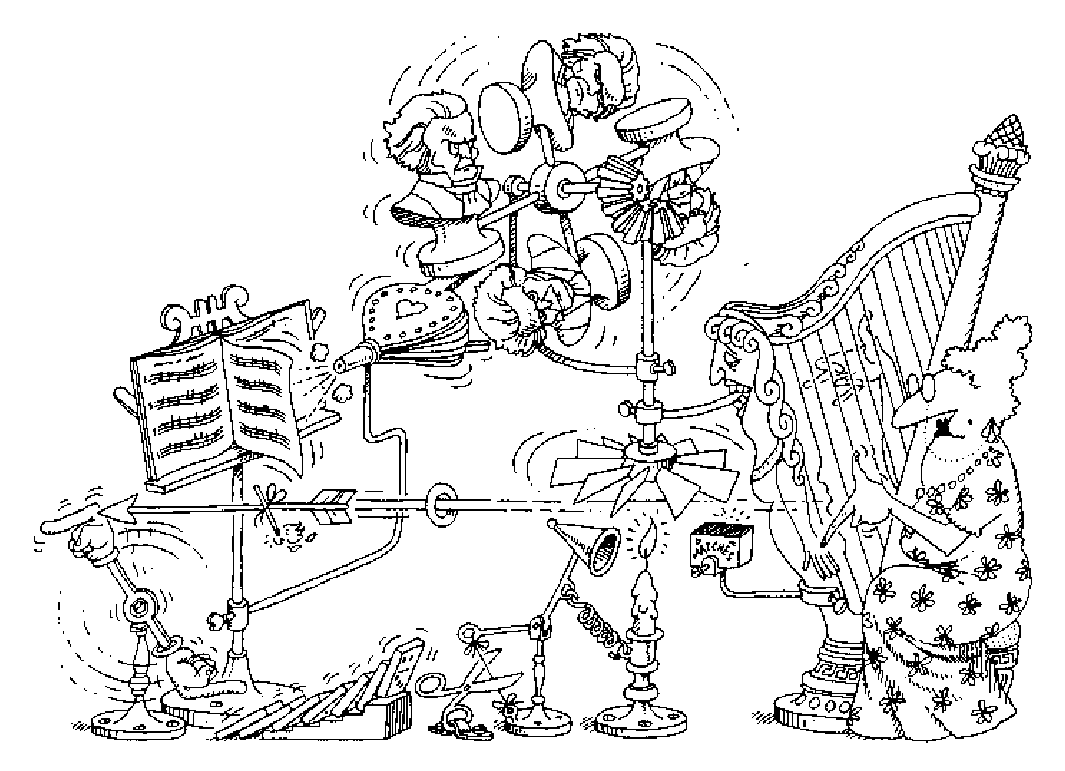
\includegraphics[width=0.9\textwidth]{cartoon7.eps}
        \caption{Mechanisms are the means whereby objects collaborate
            to provide some higher level behaviour.}
    \end{center}
\end{figure}
\begin{verbatim}
vector<StMeasuredPoint*> points;
StTrack                  *track;
MyOwnSimpleFitter        fitter;

// ... get track from somewhere ...

fillPoints(points, track);

// some print-out
for (int i=0; i<points.size(); i++)
    cout << points[i]->position() << '\t'
         << points[i]->positionError() << endl;

fitter.addPoints(points);
fitter.apply();

// ... now print the results ...
\end{verbatim}

The same scheme can be applied when you want to draw points along a helix
or sketch a helix by drawing lines between its points.\\
You can mix vertices and hits freely as long as you stick to the functionality
\texttt{StMeasuredPoint} provides.

One can now sort the hits according to their radius $\rho$ in cylindrical
coordinates. This is easy using the STL sort algorithm.\index{sort} All what is
needed is the definition of the sort 'rule': 
\begin{verbatim}
struct compareRadiusOfPoints {
    bool operator()(const StMeasuredPoint *x, const StMeasuredPoint *y) {
        return x->position().perp() < y->position().perp();
    }
};
\end{verbatim}
The following simple line does the job:
\begin{verbatim}
    sort(points.begin(), points.end(), compareRadiusOfPoints());
\end{verbatim}
\vfill
\subsection{The EMC}
\index{EMC}
... missing ...

\subsection{The RICH}
\index{RICH}
The RICH classes, like those of the EMC do not depend on
tables for their construction.  They are directly filled
into the \texttt{StEvent} structure during reconstruction and
analysis.  The \texttt{StRichCollection} is the main container class
which holds all of the objects associated with the RICH---that
is the pixels, clusters, and hits, and these are held in the
ROOT based ``STL-like'' containers within \texttt{StEvent}.
This allows internal changes to be made within the \texttt{StRichCollection}
without imposing overhead on the \texttt{StEvent} infrastructure,
or changes to other users code, so long as the persistent objects
fields do not change.

The RICH detector is in the curious situation that not all the
Monte Carlo information is available at the GEANT stage.  Specifically
a major source of background and spurious signals come from feed
back photons which are generated in the avalanche process of the
signal generation, i.e.~in
the detector simulation stage.  For this reason it is necessary
to keep track of the origin of the signals at the pixel level,
and to include the fractional contribution to all pixels from this
process at the \texttt{StEvent} level.  Because
of the relatively small data volume that the RICH produces---the order
of 1500 10 bit ADC values per central event, this is not an
overly large burden.

In the reconstruction stage of the analysis, the pixels are grouped
into \texttt{StRichCluster}s based on topology characteristics,
and from these objects, hit positions are reconstructed.
The \texttt{StRichHit}
follows the generic hit structure defined in \texttt{StEvent} for
the various detectors.  The \texttt{StRichHit} is an object
which inherits from both \texttt{StMeasuredPoint} and
\texttt{StHit}.  The position of the hit is available in STAR global
coordinates (as is required by the conventions of \texttt{StEvent})
as well as the local coordinate system of the RICH, so that analysis
using various survey geometries can occur after the \texttt{StEvent}
structure exists.  In the case of Monte Carlo generated data, which
includes embedded events, the process which spawned or contributed to
the hit is also recoverable.  In the cases of merged hits that produce
large clusters, the origin of each individual pixel can be recovered
by tracing back from the hit, to the cluster, to the pixel level.
All of these objects are kept in ROOT generated collections within
the \texttt{StRichCollection}:
\begin{itemize}
    \item \texttt{StRichHitCollection}
    \item \texttt{StRichClusterCollection}
    \item \texttt{StRichPixelCollection}
\end{itemize}
For generic studies of efficiecy
it is expected that \texttt{StMCEvent} will be utilized.  However as
mentioned previously, the addition
of pixel labelling in the internal \texttt{StRichCollection} infrastruture
will allow us to quantify, very accurately, the efficiency of utilizing
a proximity match for the basis of these calcuations, as well as study
the effect of various modes and generations of feedback photons, and
detector noise.  This labelling can also be extended to add a
parameterized neutron
background downstream of the GEANT calculation should this prove to
be a large source of additional background.

The RICH particle identification is initially expected to run
at the \texttt{StEvent} level.  The identification algorithm is currently
based on calculating the areal photon density on the RICH pad
plane for the different particle hypthesis and selecting the
most probable based on a selected set of criteria which will
not be detailed here.  This algorithm is contained in a
Maker module called the \texttt{StRICHPIDMaker} which requires
\texttt{StEvent} global tracks in addition to the \texttt{StRichCollection}
as input.

The mode of accessing this data is shown below:

\begin{verbatim}
  //
  // retrieve the StEvent data structure
  //
  StEvent* mEvent;
  mEvent = (StEvent *) GetInputDS("StRichEvent");

  if (!mEvent) {
    cout << "No StEvent*\n";
    cout << "Can not continue. Aborting..." << endl;
    return kStWarn;
  }

  //
  // Get the StRichCollection
  // 
  StRichCollection* theRichCollection = mEvent->richCollection();
  if (!theRichCollection) {
    cout << "StEvent::RichCollection does not exist\n";
    cout << "Aborting...\n" << endl;
    return kStWarn;
  }

  //
  // Get the Hits from the collection
  //
  if (!theRichCollection->hitsPresent()) {
    cout << "StRichCollection::hitCollection does not exist\n";
    cout << "Aborting...\n" << endl;
    return kStWarn;
  }

  StSPtrVecRichHit& theRichHits = theRichCollection->getRichHits();

  //
  // Get the Global Tracks
  //
  StSPtrVecTrackNode& theTrackNodes = mEvent->trackNodes();
\end{verbatim}

\subsection{The L3 Trigger}
\index{L3Trigger}

The L3Trigger class looks in essence like the ``little brother'' of
the StEvent class. It provides a subset of the data member and methods
from StEvent with respect to TPC hits, track nodes and vertices.  This
allows, to some extend, to use exactly the same analysis code for the
analysis of tracks and hits from the L3 reconstruction as for the
standard offline reconstruction chain.
The only difference is that
the user has to replace
\begin{verbatim}
     StEvent* event;
     // ...
     event->someMethod();
\end{verbatim}
with
\begin{verbatim}
     StEvent* event;
     // ...
     event->l3Trigger()->someMethod();
\end{verbatim}
Only the entry point \texttt{event} has to be replaced by \texttt{event->l3trigger()}.
However, the level of detail in the offline reconstructed data will
always be somewhat larger and some information might not be available in the L3
tree (e.g.~certain PID traits, fit traits etc.).

\subsubsection{Event Summary Information}
In addition to the track/hit information the L3 tree also contians the
complete trigger information of the algorithms switched on for the
given run and all neccessary counters for the cross section
calculataion. Global event information is stored in the \texttt{StL3EventSummary}
class, whereas detailed outcome of the algorithms is put into \texttt{StL3AlgorithmInfo}. 

Since the L3 triggered events are in general not unbiased,
e.g. the high-pt-RICH triggered events for a flow analysis,
the average user will want to sort out these event classes.
Therefore a simple member function is provided which checks how the
event decision was made: unbiased, i.e. not triggered by a L3
algorithm, or biased, i.e. triggered by L3. One exception is the L3
vertex algorithm, where a bias is not seen, or exspected, for central
events. This can be checked with a similar function.

The way to access this is shown below:
\begin{verbatim}
     StEvent* myEvent;
     myEvent = (StEvent* )chain->GetInputDS("StEvent");

     if (!myEvent) {
       cout <<"No StEvent found.\n";
       return kStWarn;  
     }

     //
     // Get L3 entry point
     //
     myL3Trigger = (StL3Trigger* )myEvent->l3Trigger();
     if (!myL3Trigger) {
       cout << "No l3 found inside StEvent.\n";
       cout << "That means l3 was switched off. \n";
       // return or continue, what ever you want
       return kStWarn;
     }

     //
     // Get L3 event summary
     //
     const StL3EventSummary* myL3EventSummary = myL3Trigger->l3EventSummary();
     if (!myL3EventSummary) {
       cout << "No l3 event summary found." << endl;
       return kStWarn;
     }

     //
     // now check the event
     //
     if (!myL3EventSummary->unbiasedTrigger()) {
       cout << "This event was triggered by L3. \n";
       cout << "Accept vertex trigger only \n";
       cout << "and skip the rest. \n";
       if (!myL3EventSummary->zVertexTrigger())
         continue;
     }
\end{verbatim}

\subsubsection{Algorithm Information}
The L3 algorithm information is stored in a pointer vector of
\texttt{StL3AlgorithmInfo} type. Access point is again the
\texttt{StL3EventSummary} class. Ideally every information for each
running algorithm is provided which is neccessary to define the
algorithm and the mode it was running in, e.g. pre/postscaling factors
and run parameters. Please note that the unique algorithm id might not
be enough to define it, since it's possible to run an algorithm twice
at the same time with different parameter sets.\\
An additional pointer vector is kept to get the information of all
algorithms which triggered the given event to save the effort of
looping over all algorithms. The following gives an example how to
access the algorithm information:
\begin{verbatim}
     //
     // Get number of algorithms switched on
     //
     unsigned int nAlgorithms = myL3EventSummary->numberOfAlgorithms(); 

     //
     // Print info for all algorithms
     //
     StSPtrVecL3AlgorithmInfo& myL3AlgInfo = myL3EventSummary->algorithms(); 
     for (int i=0; i<nAlgorithms; i++) {
       cout << " alg id " << myL3AlgInfo[i]->id()
            << ":\t #proc " << myL3AlgInfo[i]->numberOfProcessedEvents()
            << "\t #accept " << myL3AlgInfo[i]->numberOfAcceptedEvents()
            << "\t #build " << myL3AlgInfo[i]->numberOfBuildEvents()
            << endl;
     }

     //
     // Print id of triggered algorithms only
     //
     StPtrVecL3AlgorithmInfo& myL3TriggerAlgInfo;
     myL3TriggerAlgInfo = myL3EventSummary->algorithmsAcceptingEvent();
     for (int i=0; i<myL3TriggerAlgInfo->size(); i++) {
       cout << myL3TriggerAlgInfo[i]->id() << "  " << endl;
     }
\end{verbatim}

\clearpage

\section{Writing MiniDSTs using StEvent}
\label{sec:miniDST}\index{miniDST}
Following STARs terminology a miniDST is the next higher level in the
DST hierarchy after the DST itself. What follows are the
microDST and nanoDST.  The miniDST should be readable STAR-wide which
implies that it has to be based on \StEvent. This has several
advantages:
\begin{itemize}
\item programs and code that works based on \StEvent\ can be used
    directly; in fact the analysis code doesn't have to change at all
    between DST and miniDST
\item schema evolution comes for free
\item the standard IO maker handles the writing and reading of the
    miniDST
\end{itemize}

The miniDST contains a fraction of the StEvent data tree plus
(optionally) user defined components.  Which fraction of StEvent gets
written is up to the user.  The obvious candidates to go on miniDSTs
are primary tracks, vertices, or certain global tracks.  There is also
no rule which says that there can only be one miniDST. It makes
perfectly sense to keep different variants of miniDSTs. Some Physics
Working Groups might want highly compressed miniDSTs for rare probe
searches since they deal with many events. Other groups might want
more complete miniDSTs since they need less events in total.  Several
PWG can go for a common miniDST, STAR can go for a common miniDST.
This is a matter a choice.  Important is that the scheme does not
limit us in our choice that there's a way of achieving this.

The basic principle used in the implementation is not to copy and
store information in a new scheme in a different place (e.g.~in a
TTree or user defined format) but to \textbf{remove} those pieces of
the current \StEvent\ one doesn't need. The result is the same but
removing or marking instread of copying is faster and more efficient.

The extension for miniDSTs is \texttt{.mdst.root}.

\subsection{The StEventScavanger class}
\index{StEventScavanger} To get remove unwanted objects from \StEvent\ 
one can do two things: deleting them (operator \texttt{delete}) or
marking them (using the zombie mechanism).  Both methods require some
level of expertise and there are many things that can go wrong.  What
is needed is a way to savely remove arbitrary parts of StEvent in a
simple way. This is exactly what the \texttt{StEventScavanger} class
is for.

The class has only static member functions which means you can call them from
everywhere in your code without creating an instance of \texttt{StEventScavanger}.\\
Example:
\begin{verbatim}
    StEvent* event = (StEvent *) GetInputDS("StEvent");
    StEventScavenger::removeEventSummary(event);
    StEventScavenger::removeSoftwareMonitor(event);
    StEventScavenger::removeTpcHitCollection(event);
    StEventScavenger::removeFtpcHitCollection(event); 
\end{verbatim}
The class has methods to delete individual tracks, all hits, event summary,
software monitors, and much more (see section \ref{sec:StEventScavenger}).
Note, that most of these methods actually mark the objects and do not remove
via operator \texttt{delete}.
Marked objects will be ignored by the IO maker and not written
to the miniDST. So don't worry if you still see them after you called 
StEventScavenger. They won't show up on the miniDST.


\subsection{An Example: StMiniDstMaker}

The STAR library contains a complete example on how to write a miniDST.
The example consist of the \texttt{StMiniDstMaker} maker and two macros:
\texttt{mDstWrite.C} and \texttt{mDstRead.C}.

The basic idea behind the example is to show how to write a miniDST of primary kaons
which contains nothing but the kaons and the trigger information.

The most important thing is that you use the macro \texttt{mDstWrite.C} instead
of the usual \texttt{doEvents.C}-like macros. \texttt{mDstWrite.C} is especially
setup to write \StEvent\ read in from a DST into a single
output file. The version of the macro in the library calls the \texttt{StMiniDstMaker}
package to select what should be written and what not. 

So a typical run looks like this:
\begin{verbatim}
root4star -b
.x mDstWrite.C(1000,"/star/data03/reco/P00hi/2000/09","*.dst.root","mykaons");
\end{verbatim}

In this case 1000 events will be read from various\ \texttt{*.dst.root}
files in the \texttt{/star/data03/reco/P00hi/2000/09} directory and written to
a miniDST with name \texttt{mykaons.mdst.root}.
For every event the \texttt{StMiniDstMaker::Make()} method selects the kaon tracks and removes the
rest. To remove primary track which are not identified as kaons the \texttt{remove(StTrack*)} from
\texttt{StEventScavanger} class is used.
The code looks as follows:
\begin{verbatim}
    StSPtrVecPrimaryTrack& theTracks = event->primaryVertex()->daughters();
    for (unsigned int i=0; i<theTracks.size(); i++)
        if (!accept(theTracks[i]))
            StEventScavenger::remove(theTracks[i]);
\end{verbatim}

where \texttt{accept(StTrack*)} is a filter method defined in \texttt{StMiniDstMaker}.

To read the file back use for example:
\begin{verbatim}
root4star -b
.x mDstRead.C(1000,"/star/data03/reco/P00hi/2000/09","*.mdst.root");
\end{verbatim}

The \texttt{mDstRead.C} macro in the library actually calls the standard StAnalysisMaker.
Of course one can also create a macro which reads in a miniDSTs and writes out
another, more compressed version of it.\\
Please note that \texttt{StMiniDstMaker}, \texttt{mDstWrite.C}, and \texttt{mDstRead.C}
are only examples and should be used as templates for you own purposes.

\subsection{Advanced features}
\subsubsection{Using Zombies}
Most methods of the  \texttt{StEventScavanger} class are based on the 'zombie' mechanism
introduced by Victor in Sep 2000.
The scheme relies on the fact that all \StEvent\ objects inherit from \texttt{StObject}
and \texttt{StObject} itself has a few free user bits which can be used to mark the object.
Once the object is marked it becomes a zombie and will be ignored when the rest of
\StEvent\ is written to the miniDST. The object can be marked by invoking the
\texttt{void StObject::makeZombie()} method and the state of each object can be
checked with the \texttt{bool StObject::isZombie()} method.

If you feel that your understanding of StEvent is sufficient enough you always can use
the zombie mechanism directly. Once an object becomes a zombie also all references to the
object will disappear on the miniDST, i.e.~pointer are nulled, at least. In this sense
zombies are pretty save to use.

Please note, that - as in the bad movies - zombies are visible. After an object is made
a zombie you still can use the same way as before. With other words it does not get deleted
in memory.

\subsubsection{Adding user defined classes}

The miniDST mechanism is in principle not restricted to StEvent
classes only.  Objects of every class which inherits from
\texttt{StObject} and use the \texttt{ClassDef()} and
\texttt{ClassImp()} macros can be written to a miniDST. You
will need of course the class definition when you read the data back
in. If the class definition is not availabe the object cannot be
retrieved from the miniDST; you still we be able to read the rest though.
Needles to say that it is the responsibility of the user to
make sure the class is available to everyone who tries to read the
miniDSTs.

Here's a very simple example:
\begin{verbatim}
// StMyDstClass.h
#include "StObject.h"
class StMyDstClass : public StObject {
public:
    StMyDstClass();
    int myCounter;
    int eventIsGood;
    ClassDef(StMyDstClass,1);
};
\end{verbatim}

The \texttt{StMyDstClass.cxx} file of course has to exist and should contain
\begin{verbatim}
// StMyDstClass.h
#include "StMyDstClass.h"
ClassImp();
StMyDstClass::StMyDstClass()
{
    myCounter = 0;
    eventIsGood = 0;
}
\end{verbatim}

All you have to do is to create an instance of this class in the \texttt{Make()} method
of your maker (\texttt{StMiniDstMaker}) and attach it to \StEvent\:

\begin{verbatim}
StMyDstClass *my = new StMyDstClass;
my->myCounter = 17;
my->eventIsGood = 1;
event->content().push_back(my);
\end{verbatim}

From here on the \texttt{StMyDstClass} object is integral part of \StEvent\ and
will be treated as such during I/O.
Please not that you are of course not limited to build in data types
but can more complex ones as pointers to \texttt{StTrack} objects for example.
One could imagine to have a class \texttt{StMyPair} which links two tracks which form
a pair to name just one of many applications. 

\clearpage

%%%%%%%%%%%%%%%%%%%%%%%%%%%%%%%%%%%%%%%%%%%%%%%%%%%%%%%%%%%%%%%%%%%%
%
%    Reference Manual
%
%%%%%%%%%%%%%%%%%%%%%%%%%%%%%%%%%%%%%%%%%%%%%%%%%%%%%%%%%%%%%%%%%%%%
\part{Reference Manual}
\clearpage

\section{Class References} %%%%%%%%%%%%%%%%%%%%%%%%%%%%%%%%%%%%%%%%%
The classes which are currently implemented and available from the
STAR CVS repository are listed in alphabetic order.

Inherited member functions and operators are not described in the
reference section of a derived class. Always check the section(s) of
the base class(es) to get a complete overview on the available
methods.

In general each class has a public:
\begin{itemize}
\item Default constructor
\item Copy constructor
\item Assignment operator
\item Virtual destructor
\end{itemize}
There are a few exceptions from this rule which are explained in the
referring class reference.

Not every member function listed is explained in detail since many are
trivial and their names are chosen such that one can easily figure out
what they are all about.  Macros and \texttt{Inline} declarations are
omitted throughout the documentation and so is the \texttt{virtual}
keyword.  The state-of-the-art reference is always the class
definition in the header file.
\begin{figure}[htb]
    \begin{center}
        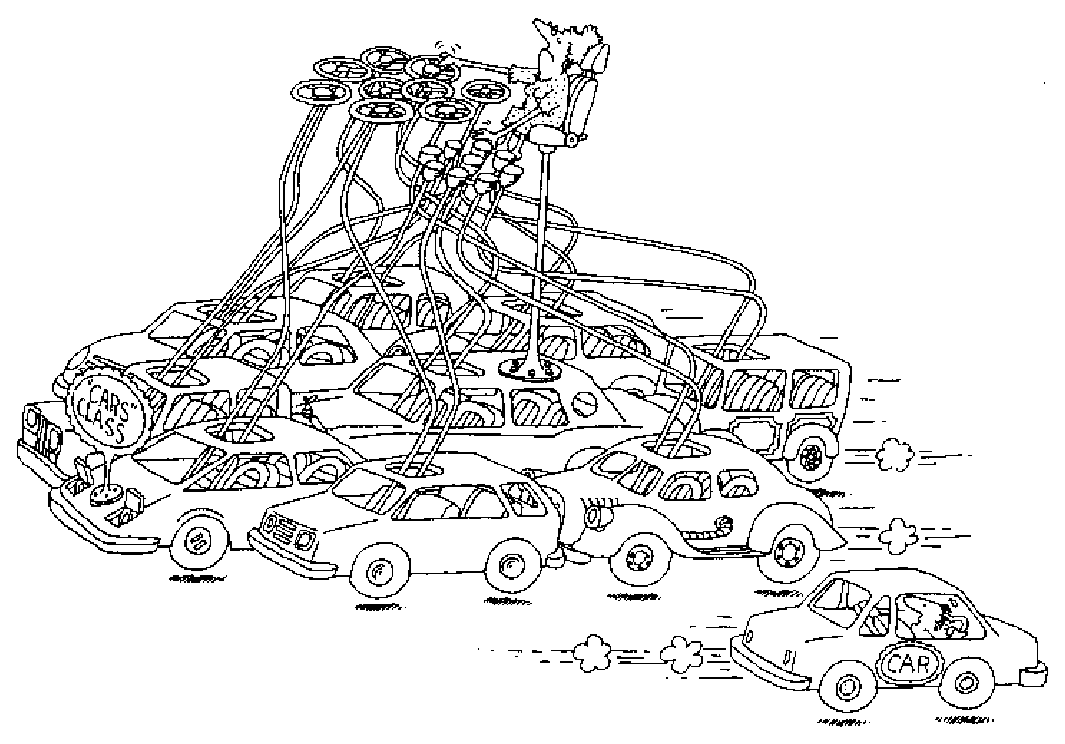
\includegraphics[width=0.8\textwidth]{cartoon8.eps}
        \caption{A class represents a set of objects that share
            a common structure and a common behavior.}
    \end{center}
\end{figure}
\clearpage

\subsection{StBbcTriggerDetector}
\index{StBbcTriggerDetector|textbf}
\label{sec:StBbcTriggerDetector}
\begin{Entry}
\item[Summary]
\item[Synopsis]
    \verb+#include "StBbcTriggerDetector.h"+\\
    \verb+class StBbcTriggerDetector;+\\
\item[Description]
\item[Related Classes]
\item[Public\\ Constructors]
    \verb+StBbcTriggerDetector();+\\
\item[Public Member\\ Functions]
    \verb+unsigned int numberOfPMTs() const;+\\
    \verb+unsigned int numberOfRegisters() const;+\\
    \verb+unsigned int numberOfPedestalData() const;+\\
    \verb+unsigned int numberOfScalars() const;+\\
    \verb+unsigned short adc(unsigned int) const;+\\
    \verb+unsigned short tdc(unsigned int) const;+\\
    \verb+unsigned short bbcRegister(unsigned int) const;+\\
    \verb+unsigned short pedestalData(unsigned int) const;+\\
    \verb+unsigned int scalar(unsigned int) const;+\\
    \verb+unsigned short pedestal(unsigned int id) const;+\\
    \verb+unsigned short pedestalWidth(unsigned int id) const;+\\
    \verb+unsigned short mip(unsigned int id) const;+\\
    \verb+unsigned short mipWidth(unsigned int id) const;+\\
    \verb+int nHitEast();+\\
    \verb+int nHitWest();+\\
    \verb+int nHitAll();+\\
    \verb+int adcSumEast(); +\\
    \verb+int adcSumWest();+\\
    \verb+int adcSumAll();+\\
    \verb+float zVertex(); //z vertex in cm+\\
    \verb+void setAdc(unsigned int, unsigned short);+\\
    \verb+void setTdc(unsigned int, unsigned short);+\\
    \verb+void setRegister(unsigned int, unsigned short);+\\
    \verb+void setPedestal(unsigned int, unsigned short);+\\
    \verb+void setScalar(unsigned int, unsigned int);+\\
    \verb+void dump();+\\
\end{Entry}
\clearpage

\subsection{StCalibrationVertex}
\index{StCalibrationVertex|textbf}
\label{sec:StCalibrationVertex}
\begin{Entry}
\item[Summary]
    Represents vertices used for test and calibration purposes.
    
\item[Synopsis]
    \verb+#include "StCalibrationVertex.h"+\\
    \verb+class StCalibrationVertex;+\\
    
\item[Description]
    Concrete implementatin of the \texttt{StVertex} class.
    It represents various types of vertices useful for calibration and
    diagnostics. These vertices have no daughters and no parent.  All
    vertices of this category are of type \texttt{kOtherVtxId} (see
    \texttt{StVertex::type()}).  Don't worry if you don't what they
    are good for.  There are nor relevant for physics analysis.
    
\item[Related Classes]
    Inherits from \texttt{StVertex}. \texttt{StCalibrationVertex} doesn't add
    any new data member of methods. 
    
\item[Public\\ Constructors]
    \verb+StCalibrationVertex();+\\
    \verb+StCalibrationVertex(const dst_vertex_st&);+\\
    
\item[Public Member\\ Functions]
    See \texttt{StVertex} (\ref{sec:StVertex}) for available methods.
\end{Entry}
\clearpage

\subsection{StContainers}
\index{StContainers|textbf}
\label{sec:StContainers}
\begin{Entry}
\item[Summary] Definitions of all container types used in \StEvent.
\item[Synopsis]
    \verb+#include "StContainers.h"+\\
\item[Description] \texttt{StContainers.h} includes \texttt{StArray.h}
    which contains the guts of the container implementation. In
    StContainer.h (and .cxx) the appropriate macros are called to
    declare and define the container types. If a new container type
    has to be defined it \emph{must} be defined here and only here.
\end{Entry}
\clearpage


\subsection{StCtbSoftwareMonitor}
\index{StCtbSoftwareMonitor|textbf}
\label{sec:StCtbSoftwareMonitor}
\begin{Entry}
\item[Summary] Monitors details of the Central Trigger Barrel (CTB)
    reconstruction.
\item[Synopsis]
    \verb+#include "StCtbSoftwareMonitor.h"+\\
    \verb+class StCtbSoftwareMonitor;+\\
\item[Description]
\item[Related Classes]
\item[Public\\ Constructors]
    \verb+StCtbSoftwareMonitor();+\\

    \verb+StCtbSoftwareMonitor(const dst_mon_soft_ctb_st&);+\\
\item[Public Data\\ Member]
    \verb+int mult_ctb_tot;+\\
    Total multiplicity (or ADC sum) in CTB.
\end{Entry}
\clearpage


\subsection{StCtbTriggerDetector}
\index{StCtbTriggerDetector|textbf}
\label{sec:StCtbTriggerDetector}
\begin{Entry}
\item[Summary] Interface to CTB event data.
    
\item[Synopsis]
    \verb+#include "StCtbTriggerDetector.h"+\\
    \verb+class StCtbTriggerDetector;+\\
\item[Description]
    
\item[Related Classes]
    Inherits from StObject.
    
\item[Public\\ Constructors]
    \verb+StCtbTriggerDetector();+\\
    \verb+StCtbTriggerDetector(const dst_TrgDet_st&);+\\
    
\item[Public Member\\ Functions]
    \verb+unsigned int numberOfTrays() const;+\\
    Returns number of CTB trays (usually 120).
    
    \verb+unsigned int numberOfSlats() const;+\\
    Returns number of slats (usually 2).
    
    \verb+unsigned int numberOfPreSamples() const;+\\
    Number of pre-samples taken.
    
    \verb+unsigned int numberOfPostSamples() const;+\\
    Number of post-samples taken.
    
    \verb+unsigned int numberOfAuxWords() const;+\\
    Number of auxiliary words (usually 16).  No physical significance
    at present, these data are simple reserved for possible future
    use.
    
    \verb+float mips(unsigned int tr, unsigned int sl, unsigned int evt = 0) const;+\\
    Return MIPS for tray \texttt{tr} and slot \texttt{sl}.  The trays
    run from 0 -- \texttt{numberOfTrays()}-1, the slots from 0 --
    \texttt{numberOfSlots()}-1. The first half of the tray numbers are
    for the west side, the second half for the east side (usually 0-59
    on west end, 60-119 on east end).  Each tray has 2 slats, 0 is the
    inner slat, closest to the central membrane, and 1 is the outer
    slat, further from the central membrane.  The last argument
    \texttt{evt} has  the following meaning:\\
    0 is the triggered event, and
    from 1 to \texttt{(npresamples+npostsamples)} are the other "events",
    in chronological order.  For example, assuming 5 pre events and 5
    post events:
    \begin{description}
    \item[evt = 0] triggered event at t = 0
    \item[evt = 1] 1st pre event at t = -5
    \item[evt = 2] 2nd pre event at t = -4
    \item[evt = 3] 3rd pre event at t = -3
    \item[evt = 4] 1st post event at t = -2
    \item[evt = 5] 2nd post event at t = -1
    \item[evt = 6] 2nd post event at t = +1
    \item[evt = 7] 2nd post event at t = +2
    \item[evt = 8] 2nd post event at t = +3
    \item[evt = 9] 2nd post event at t = +4
    \item[evt = 10] 2nd post event at t = +5
    \end{description}
    
    \verb+char time(unsigned int tray, unsigned int slot, unsigned int evt = 0) const;+\\
    Same arguments as for \texttt{mips()} (see above).
     
    \verb+float aux(unsigned int, unsigned int evt = 0) const;+\\
    Argument \texttt{i} has no physical significance at present, these
    data are simple reserved (on request of Hank Crawford) for
    possible future use.  For the second argument (\texttt{evt}) see
    \texttt{mips()} above.

    \verb+void setMips(unsigned int, unsigned int, unsigned int, float);+\\
    \verb+void setTime(unsigned int, unsigned int, unsigned int, char);+\\
    \verb+void setAux(unsigned int, unsigned int, float);+\\
    \verb+void setNumberOfPreSamples(unsigned int);+\\
    \verb+void setNumberOfPostSamples(unsigned int);+\\
\end{Entry}
\clearpage



\subsection{StDedxPidTraits}
\index{StDedxPidTraits|textbf}
\label{sec:StDedxPidTraits}
\begin{Entry}
\item[Summary]
\item[Synopsis]
    \verb+#include "StDedxPidTraits.h"+\\
    \verb+class StDedxPidTraits;+\\
\item[Description]
\item[Related Classes]
\item[Public\\ Constructors]
    \verb+StDedxPidTraits();+\\
    Default constructor.
    
    \verb+StDedxPidTraits(StDetectorId det, short emethod,+\\
    \verb+                unsigned short np, float dedx, float sig);+\\
    Create an instance of \texttt{StDedxPidTraits} for detector
    \texttt{det}, encoded method \texttt{emethod}, number of points
    \texttt{np}, dE/dx mean \texttt{dedx}, and error on mean \texttt{sig}.
    
\item[Public Member\\ Functions]
    \verb+unsigned short numberOfPoints() const;+\\
    Number of points used to calculate the dE/dx value.
    
    \verb+float mean() const;+\\
    The derived dE/dx value.

    \verb+float length() const;+\\
    Track length used in dE/dx calculations.
    
    \verb+float errorOnMean() const;+\\
    Returns the error on the dE/dx value.
    
    \verb+StDedxMethod method() const;+\\    

    \verb+short encodedMethod() const;+\\
\end{Entry}
\clearpage

\subsection{StDetectorState}
\index{StDetectorState|textbf} \index{detector state}
\label{sec:StDetectorState}
\begin{Entry}
\item[Summary] Base class for detector state information.
\item[Synopsis]
    \verb+#include "StDetectorState.h"+\\
    \verb+class StDetectorState;+\\
\item[Description]
    \texttt{StDetectorState} is a non-abstract base class to hold information
    on the ``state'' of a detector. All concrete classes reflecting the state
    of actual detectors need to inherit from this class in order to allow
    storage in \texttt{StEvent}. The only data member it contains are the detector ID
    and a Boolean to reflect the overall state (good/bad). More detailed
    information may be added by the derived classes.
    
\item[Related Classes]
\item[Public\\ Constructors]
    \verb+StDetectorState();+\\
    \verb+StDetectorState(StDetectorId, bool);+\\
    
\item[Public Member\\ Functions]
    \verb+StDetectorId detector() const;+\\
    Returns detector ID (see \ref{sec:Enumerations}).
    
    \verb+bool good() const;+\\
    Return \texttt{true} if the overall state of the detector is good, otherwise \texttt{false}.
    
    \verb+bool bad() const;+\\
    Returns the negative of \texttt{good()}.
    
    \verb+void setDetector(StDetectorId);+\\
    \verb+void setGood(bool);+\\
\end{Entry}
\clearpage

\subsection{StEmcCluster}
\index{StEmcCluster|textbf}
\label{sec:StEmcCluster}
\begin{Entry}
\item[Summary]
\item[Synopsis]
    \verb+#include "StEmcCluster.h"+\\
    \verb+class StEmcCluster;+\\
\item[Description]
\item[Related Classes]
\item[Public\\ Constructors]
    \verb+StEmcCluster();+\\
\item[Public Member\\ Functions]
    \verb+float eta() const;+\\
    \verb+float phi() const;+\\
    \verb+float sigmaEta() const;+\\
    \verb+float sigmaPhi() const;+\\
    \verb+float energy() const;+\\
    \verb+int nHits() const; +\\
    \verb+int nNeighbors() const;+\\
    \verb+int nTracks() const;+\\
    \verb+StPtrVecEmcRawHit& hit();+\\
    \verb+const StPtrVecEmcRawHit& hit() const;+\\
    \verb+StPtrVecEmcCluster& neighbor();+\\
    \verb+const StPtrVecEmcCluster& neighbor() const;+\\
    \verb+StPtrVecTrack& track();+\\
    \verb+const StPtrVecTrack& track() const;+\\
    \verb+void setEta(float);+\\
    \verb+void setPhi(float);+\\
    \verb+void setSigmaEta(float);+\\
    \verb+void setSigmaPhi(float);+\\
    \verb+void setEnergy(float);+\\
    \verb+void addHit(StEmcRawHit*);+\\
    \verb+void addNeighbor(StEmcCluster*);+\\
    \verb+void addTrack(StTrack*);+\\
    \verb+void print(ostream& os = cout) const;+\\
\end{Entry}
\clearpage


\subsection{StEmcClusterCollection}
\index{StEmcClusterCollection|textbf}
\label{sec:StEmcClusterCollection}
\begin{Entry}
\item[Summary]
\item[Synopsis]
    \verb+#include "StEmcClusterCollection.h"+\\
    \verb+class StEmcClusterCollection;+\\
\item[Description]
\item[Related Classes]
\item[Public\\ Constructors]
    \verb+StEmcClusterCollection();+\\
\item[Public Member\\ Functions]
    \verb+StDetectorId detector() const;+\\
    \verb+void setDetector(StDetectorId);+\\
    \verb+int numberOfClusters() const;+\\
    \verb+StSPtrVecEmcCluster& clusters();+\\
    \verb+const StSPtrVecEmcCluster& clusters() const;+\\
    \verb+void addCluster(StEmcCluster*);+\\
    \verb+int clusterFinderId() const;+\\
    \verb+int clusterFinderParamVersion() const;+\\
    \verb+void setClusterFinderId(int);+\\
    \verb+void setClusterFinderParamVersion(int);+\\
\end{Entry}
\clearpage


\subsection{StEmcCollection}
\index{StEmcCollection|textbf}
\label{sec:StEmcCollection}
\begin{Entry}
\item[Summary]
\item[Synopsis]
    \verb+#include "StEmcCollection.h"+\\
    \verb+class StEmcCollection;+\\
\item[Description]
\item[Related Classes]
\item[Public\\ Constructors]
    \verb+StEmcCollection();+\\
\item[Public Member\\ Functions]
    \verb+StEmcDetector* detector(StDetectorId);+\\
    \verb+const StEmcDetector* detector(StDetectorId) const;+\\
    \verb+StSPtrVecEmcPoint& barrelPoints();+\\
    \verb+const StSPtrVecEmcPoint& barrelPoints() const;+\\
    \verb+StSPtrVecEmcPoint& endcapPoints();+\\
    \verb+const StSPtrVecEmcPoint& endcapPoints() const;+\\
    \verb+void addBarrelPoint(const StEmcPoint*);+\\
    \verb+void addEndcapPoint(const StEmcPoint*);+\\
    \verb+void setDetector(StEmcDetector*);+\\
\end{Entry}
\clearpage


\subsection{StEmcDetector}
\index{StEmcDetector|textbf}
\label{sec:StEmcDetector}
\begin{Entry}
\item[Summary]
\item[Synopsis]
    \verb+#include "StEmcDetector.h"+\\
    \verb+class StEmcDetector;+\\
\item[Description]
\item[Related Classes]
\item[Public\\ Constructors]
    \verb+StEmcDetector();+\\
    \verb+StEmcDetector(StDetectorId, unsigned int);+\\
\item[Public Member\\ Functions]
    \verb+StDetectorId detectorId() const;+\\
    \verb+unsigned int numberOfModules() const;+\\
    \verb+bool addHit(StEmcRawHit*);+\\
    \verb+unsigned int numberOfHits() const;+\\
    \verb+StEmcModule* module(unsigned int);+\\
    \verb+const StEmcModule* module(unsigned int) const;+\\
    \verb+StEmcClusterCollection* cluster();+\\
    \verb+const StEmcClusterCollection* cluster() const;+\\
    \verb+void setCluster(StEmcClusterCollection*);+\\
\end{Entry}
\clearpage


\subsection{StEmcModule}
\index{StEmcModule|textbf}
\label{sec:StEmcModule}
\begin{Entry}
\item[Summary]
\item[Synopsis]
    \verb+#include "StEmcModule.h"+\\
    \verb+class StEmcModule;+\\
\item[Description]
\item[Related Classes]
\item[Public\\ Constructors]
    \verb+StEmcModule();+\\
\item[Public Member\\ Functions]
    \verb+unsigned int numberOfHits() const;+\\
    \verb+StSPtrVecEmcRawHit& hits();+\\
    \verb+const StSPtrVecEmcRawHit& hits() const;+\\
\end{Entry}
\clearpage


\subsection{StEmcPoint}
\index{StEmcPoint|textbf}
\label{sec:StEmcPoint}
\begin{Entry}
\item[Summary]
\item[Synopsis]
    \verb+#include "StEmcPoint.h"+\\
    \verb+class StEmcPoint;+\\
\item[Description]
\item[Related Classes]
\item[Public\\ Constructors]
    \verb+StEmcPoint();+\\
    \verb+StEmcPoint(const StThreeVectorF&,+\\
    \verb+           const StThreeVectorF&,+\\
    \verb+           const StThreeVectorF&,+\\
    \verb+           unsigned int, float,+\\
    \verb+           float, float,+\\
    \verb+           unsigned char = 0);+\\
\item[Public Member\\ Functions]
    \verb+float energy() const;+\\
    \verb+float chiSquare() const;+\\
    \verb+void setEnergy(const float);+\\
    \verb+void setChiSquare(const float);+\\
    \verb+StThreeVectorF size() const;+\\
    \verb+void setSize(const StThreeVectorF&);+\\
    \verb+float energyInDetector(const StDetectorId) const;+\\
    \verb+float sizeAtDetector(const StDetectorId) const;+\\
    \verb+void setEnergyInDetector(const StDetectorId, const float);+\\
    \verb+void setSizeAtDetector(const StDetectorId, const float);+\\
    \verb+StPtrVecEmcCluster& cluster(const StDetectorId);+\\
    \verb+const StPtrVecEmcCluster& cluster(const StDetectorId) const;+\\
    \verb+void addCluster(const StDetectorId, const StEmcCluster*);+\\
    \verb+StPtrVecEmcPoint& neighbor();+\\
    \verb+const StPtrVecEmcPoint& neighbor() const;+\\
    \verb+void addNeighbor(const StEmcPoint*);+\\
    \verb+int nTracks() const;+\\
    \verb+StPtrVecTrack& track();+\\
    \verb+const StPtrVecTrack& track() const;+\\
    \verb+void addTrack(StTrack*);+\\
\end{Entry}
\clearpage


\subsection{StEmcRawHit}
\index{StEmcRawHit|textbf}
\label{sec:StEmcRawHit}
\begin{Entry}
\item[Summary]
\item[Synopsis]
    \verb+#include "StEmcRawHit.h"+\\
    \verb+class StEmcRawHit;+\\
\item[Description]
\item[Related Classes]
\item[Public\\ Constructors]
    \verb+StEmcRawHit();+\\
    \verb+StEmcRawHit(StDetectorId, unsigned int, unsigned int, unsigned int, unsigned int);+\\
    \verb+StEmcRawHit(StDetectorId, unsigned int, unsigned int, unsigned int, unsigned int, float);+\\
\item[Public Member\\ Functions]
    \verb+StDetectorId detector() const;+\\
    \verb+unsigned int module() const;+\\
    \verb+unsigned int eta() const;+\\
    \verb+unsigned int sub() const;+\\
    \verb+unsigned int adc() const;+\\
    \verb+float energy() const;+\\
    \verb+void setId(StDetectorId, unsigned int, unsigned int, unsigned int);+\\
    \verb+void setAdc(const unsigned int);+\\
    \verb+void setEnergy(const float);+\\
\end{Entry}
\clearpage


\subsection{StEmcSoftwareMonitor}
\index{StEmcSoftwareMonitor|textbf}
\label{sec:StEmcSoftwareMonitor}
\begin{Entry}
\item[Summary]
\item[Synopsis]
    \verb+#include "StEmcSoftwareMonitor.h"+\\
    \verb+class StEmcSoftwareMonitor;+\\
\item[Description]
\item[Related Classes]
\item[Public\\ Constructors]
    \verb+StEmcSoftwareMonitor();+\\
    \verb+StEmcSoftwareMonitor(const dst_mon_soft_emc_st&);+\\
\item[Public Data\\ Member]
    \verb+float energy_emc;+\\
    Total energy (or ADC sum) in EMC.
\end{Entry}
\clearpage


\subsection{StEnumerations}
\index{StEnumerations|textbf}
\label{sec:StEnumerations}
\begin{Entry}
\item[Summary] Header file which contains all enumeration types used
    in \StEvent.
\item[Synopsis]
    \verb+#include "StEnumerations.h"+\\
\item[Description] All enumeration types used in \StEvent\ are defined
    in this header file. It also includes other header files which are
    common to all STAR code. For a complete list of enum types see
    section \ref{sec:Enumerations}.
\end{Entry}
\clearpage

\subsection{StEmcTriggerDetector}
\index{StEmcTriggerDetector|textbf}
\label{sec:StEmcTriggerDetector}
\begin{Entry}
\item[Summary]
\item[Synopsis]
    \verb+#include "StEmcTriggerDetector.h"+\\
    \verb+class StEmcTriggerDetector;+\\
\item[Description]
\item[Related Classes]
\item[Public\\ Constructors]
    \verb+StEmcTriggerDetector();+\\
    \verb+StEmcTriggerDetector(const dst_TrgDet_st&);+\\
\item[Public Member\\ Functions]
    \verb+int numberOfTowers() const;+\\
    \verb+int highTower(unsigned int) const;+\\
    \verb+int patch(unsigned int) const;+\\
    \verb+void setHighTower(unsigned int, int);+\\
    \verb+void setPatch(unsigned int, int);+\\
\end{Entry}
\clearpage

\subsection{StEvent}
\index{StEvent|textbf}
\label{sec:StEvent}
\begin{Entry}
\item[Summary] Event header and entry point to the \StEvent\ tree.
\item[Synopsis]
    \verb+#include "StEvent.h"+\\
    \verb+class StEvent;+\\
\item[Description] The class \texttt{StEvent} is the key class to work
    with the whole \StEvent\ tree. It itself contains data which
    describes and characterizes the event and gives references and
    pointers to all information there is in the event.  Don't forget
    to check for \texttt{NULL} pointers if a method returns an object
    by pointer. Only if a method returns an object by reference
    it is guaranteed to exist.\\
    The package StEventMaker (see Sec.~\ref{sec:StEventMaker})
    provides a pointer to the current instance of \texttt{StEvent}.
\item[Related Classes] Class \texttt{StEvent} inherits from
    \texttt{St\_DataSet}.
\item[Public\\ Constructors]
    \verb+StEvent();+\\
    
    \verb+StEvent(const event_header_st&,+\\
    \verb+        const dst_event_summary_st&,+\\
    \verb+        const dst_summary_param_st&);+\\
    
    \verb+StEvent(const event_header_st&);+\\
    
\item[Public Member\\ Functions]
    \verb+void Browse(TBrowser*);+\\
    Overwrite inherited \texttt{Browse()} method from \texttt{St\_DataSet}.
    Method is invoked from ROOT to allow interactive browsing of \StEvent. 

    \verb+static const TString& cvsTag();+\\
    CVS tag of the version you are using.
    
    \verb+void statistics() const;+\\
    Prints information to \texttt{cout}, as number of tracks, hits,
    vertices, event and run ID, time, and more. This method can be also
    invoked from the ROOT GUI.
    
    \verb+const TString& type() const;+\\
    Character string which contains a short description of the type of
    the event you got.
    
    \verb+int id() const;+\\
    Unique event identifier.
    
    \verb+int runId() const;+\\
    Unique run identifier.
    
    \verb+int time() const;+\\
    Time when the event was taken. The format depends pretty much
    on the DST version. Older DST version return HHMMSS while newer
    runs will return the standard UNIX time. For the latter one then
    is able to use the many UNIX standard tools available for this
    time format (e.g.~\texttt{ctime()}).
    
    \verb+unsigned int triggerMask() const;+\\

    \verb+unsigned int bunchCrossingNumber(Uint_t i) const;+\\       
    Returns the bunch crossing numbers, i.e.~two 32 bit words.
    \texttt{i = 0} returns the lower and \texttt{i = 1} the upper number.

    \verb+StEventSummary* summary();+\\
    \verb+const StEventSummary* summary() const;+\\
    Returns pointer to the event summary with many useful information
    for QA/QC and event characterization.

    \verb+StEventInfo* info();+\\
    \verb+const StEventInfo* info() const;+\\
    Returns a pointer to the one and only instance of \texttt{StEventInfo}.
    \texttt{StEventInfo} provides no additional information but is solely
    used to hold the header data. Some info can also be directly obtained  from
    StEvent. See also \ref{sec:StEventInfo}.
    \index{StEventInfo}

    \verb+StRunInfo* runInfo();+\\
    \verb+const StRunInfo* runInfo() const;+\\
    Returns a pointer to the one and only instance of \texttt{StRunInfo}.
    \texttt{StRunInfo} contains parameters related to the current run.
    See also \ref{sec:StRunInfo}.
    \index{StRunInfo}

    \verb+StSoftwareMonitor* softwareMonitor();+\\
    \verb+const StSoftwareMonitor* softwareMonitor() const;+\\
    Returns pointer to the software-monitor collection. This class
    holds ``monitors'' for every detector which contain information
    gathered during the event reconstruction. Mostly statistic on
    number of hits, tracks etc.
    
    \verb+StTpcHitCollection* tpcHitCollection();+\\
    \verb+const StTpcHitCollection* tpcHitCollection() const;+\\
    Pointer to the TPC hit collection. If no hits are stored on the
    DST this pointer is \texttt{NULL}. You better check for this.
    
    \verb+StFtpcHitCollection* ftpcHitCollection();+\\
    \verb+const StFtpcHitCollection* ftpcHitCollection() const;+\\
    Pointer to the FTPC hit collection. If no hits are stored on the
    DST this pointer is \texttt{NULL}. You better check for this.

    \verb+StSvtHitCollection* svtHitCollection();+\\
    \verb+const StSvtHitCollection* svtHitCollection() const;+\\
    Pointer to the SVT hit collection. If no hits are stored on the
    DST this pointer is \texttt{NULL}. You better check for this.    

    \verb+StSsdHitCollection* ssdHitCollection();+\\
    \verb+const StSsdHitCollection* ssdHitCollection() const;+\\
    Pointer to the SSD hit collection. If no hits are stored on the
    DST this pointer is \texttt{NULL}. You better check for this.   

    \verb+StRichCollection* richCollection();+\\
    \verb+const StRichCollection* richCollection() const;+\\

    \verb+StTofCollection* tofCollection();+\\
    \verb+const StTofCollection* tofCollection() const;+\\

    \verb+StFpdCollection* fpdCollection();+\\
    \verb+const StFpdCollection* fpdCollection() const;+\\

    \verb+StL0Trigger* l0Trigger();+\\
    \verb+const StL0Trigger* l0Trigger() const;+\\

    \verb+StL3Trigger* l3Trigger();+\\
    \verb+const StL3Trigger* l3Trigger() const;+\\

    \verb+StTriggerDetectorCollection* triggerDetectorCollection();+\\
    \verb+const StTriggerDetectorCollection* triggerDetectorCollection() const;+\\
    Returns pointer to the current trigger detector collection.
    Trigger detectors are CTB, ZDC, VPD, and MWC.
    
    \verb+StSPtrVecTrackDetectorInfo& trackDetectorInfo();+\\
    \verb+const StSPtrVecTrackDetectorInfo& trackDetectorInfo() const;+\\
    
    \verb+StSPtrVecTrackNode& trackNodes();+\\
    \verb+const StSPtrVecTrackNode& trackNodes() const;+\\
    
    \verb+unsigned int numberOfPrimaryVertices() const;+\\
    Number of primary vertices (aka event vertices).  Usually there is
    only one but future implementations of the vertex finder will be
    able to also detect pile-up vertices in which case you better
    check the number before dealing with the event.
    
    \verb+StPrimaryVertex* primaryVertex(unsigned int i = 0);+\\
    \verb+const StPrimaryVertex* primaryVertex(unsigned int i = 0) const;+\\
    Returns pointer to the \texttt{i}'th primary vertex.  Since in
    most of the cases there is only one primary vertex \texttt{i}
    defaults to the first (\texttt{i=0}).\\
    The primary vertices are ordered according to the number of daughters
    (i.e.~primary tracks) they hold. The first in the list is always the
    the vertex with the most daughter tracks.\index{primary vertices, order of}

    \verb+unsigned int numberOfCalibrationVertices() const;+\\
    Number of vertices stored for calibration and test purposes.
    
    \verb+StCalibrationVertex* calibrationVertex(unsigned int i);+\\
    \verb+const StCalibrationVertex* calibrationVertex(unsigned int i) const;+\\
    Returns pointer to the \texttt{i}'th 'calibration' vertex. Calibration
    vertices are of type \texttt{StCalibrationVertex} (see \ref{sec:StCalibrationVertex})
    and are mainly used for test, calibration, and diagnosis. Not relevant for physics analysis.
    
    \verb+StSPtrVecV0Vertex& v0Vertices();+\\
    \verb+const StSPtrVecV0Vertex& v0Vertices() const;+\\
    Returns container with V0 vertices.
    
    \verb+StSPtrVecXiVertex& xiVertices();+\\
    \verb+const StSPtrVecXiVertex& xiVertices() const;+\\
    Returns container with Xi vertices.
    
    \verb+StSPtrVecKinkVertex& kinkVertices();+\\
    \verb+const StSPtrVecKinkVertex& kinkVertices() const;+\\
    Returns container with kink vertices.

    \verb+StSPtrVecObject& content();+\\
    Returns the content of \texttt{StEvent}. Use with great care!\\
    The class \texttt{StEvent} itself is, technically spoken, not
    much more than a container of objects of type \texttt{StObject}.
    It is the level of sophistication in the member functions
    which gives the class its look-and-feel. Any class inheriting
    from \texttt{StObject} can be added to StEvent and such be made
    persistent. To add use:\\
    \texttt{StEvent::content().push\_back(StObject*);}\\
    Of course it is now also your job to retrieve the object from the
    list. This is best done using the C++ RTTI mechanism.
    
    \verb+StDetectorState*  detectorState(StDetectorId det);+\\
    \verb+const StDetectorState*  detectorState(StDetectorId det) const;+\\
    Returns pointer to detector ``state'' object referring to detector \texttt{det}.
    For \texttt{StDetectorId} see \ref{sec:Enumerations}. Note that returned pointer
    might point to a class derived from \texttt{StDetectorState}. In this case
    a \texttt{dynamic\_cast} is required unless you are only interested in the overall
    detector state which is obtained via \texttt{StDetectorState::good()}.
    If no ``state'' object for the referring detector is available a NULL pointer
    is returned.

    \verb+StPsd*  psd(StPwg pwg, int id);+\\ 
    \verb+const StPsd* psd(StPwg pwg, int id) const;+\\
    Retrieve Physics Summary Data (PSD) from physics working group \texttt{pwg}
    (for \texttt{StPwg} see \ref{sec:Enumerations}) with identifier \texttt{id}.
    Returns \texttt{null} if not present.
    \index{Physics Summary Data (PSD)}
    \index{PSD}
        
    \verb+unsigned int numberOfPsds();+\\
    Returns number of all PSDs stored in \texttt{StEvent}.

    \verb+unsigned int numberOfPsds(StPwg pwg);+\\ 
    Returns number of all PSDs from Physics Working Group \texttt{pwg} stored in \texttt{StEvent}.

    \verb+void setType(const char*);+\\

    \verb+void setRunId(int);+\\

    \verb+void setId(int);+\\

    \verb+void setTime(int);+\\

    \verb+void setTriggerMask(unsigned int);+\\

    \verb+void setBunchCrossingNumber(unsigned int, unsigned int);+\\

    \verb+void setSummary(StEventSummary*);+\\

    \verb+void setInfo(StEventInfo*);+\\
    
    \verb+void setRunInfo(StRunInfo*);+\\

    \verb+void setSoftwareMonitor(StSoftwareMonitor*);+\\

    \verb+void setTpcHitCollection(StTpcHitCollection*);+\\

    \verb+void setFtpcHitCollection(StFtpcHitCollection*);+\\

    \verb+void setSvtHitCollection(StSvtHitCollection*);+\\

    \verb+void setRichCollection(StRichCollection*);+\\

    \verb+void setTofCollection(StTofCollection*);+\\

    \verb+void setFpdCollection(StFpdCollection*);+\\

    \verb+void setTriggerDetectorCollection(StTriggerDetectorCollection*);+\\

    \verb+void setL0Trigger(StL0Trigger*);+\\
    
    \verb+void setL3Trigger(StL3Trigger*);+\\
    
    \verb+void addPrimaryVertex(StPrimaryVertex*);+\\
    Adds a primary vertex to the list. The vertices are
    automatically sorted according to their number of daughter
    tracks (descending order). \index{primary vertices, sorting}

    \verb+void addCalibrationVertex(StCalibrationVertex*);+\\

    \verb+void addDetectorState(StDetectorState*);+\\
    
    \verb+void addPsd(StPsd* psd);+\\
    Add PSD \texttt{*psd} to StEvent. This method checks if another
    PSD with identical identifiers is already stored. If so, it prints
    an error message and doesn't add the object pointed to by
    \texttt{psd}. Note that after this call the object is owned by StEvent.
    Don't delete it. However, you can still modify it.
    
    \verb+void removePsd(StPsd* psd);+\\
    Removes PSD pointed to by \texttt{psd}. Please note that \texttt{psd}
    itself is not nulled. The pointer is not valid anymore once this method
    was invoked.
    
\end{Entry}
\clearpage

\subsection{StEventInfo}
\index{StEventInfo|textbf}
\label{sec:StEventInfo}
\begin{Entry}
\item[Summary] StEvent header info

\item[Synopsis]
    \verb+#include "StEventInfo.h"+\\
    \verb+class StEventInfo;+\\
    
\item[Description]
    Please note that some information this class
    provides is already accessible directly through the
    \texttt{StEvent} class itself. This class is used hold general
    event related information within \texttt{StEvent} such as event
    and run number, event size, and the time the event was recorded.
    For more information see \ref{sec:StEvent}.

\item[Related Classes]
\item[Public\\ Constructors]
    \verb+StEventInfo();+\\
    \verb+StEventInfo(const event_header_st&);+\\
\item[Public Member\\ Functions]
    \verb+const TString& type() const;+\\
    \verb+int id() const;+\\
    \verb+int runId() const;+\\
    \verb+int time() const;+\\
    \verb+unsigned int triggerMask() const;+\\
    \verb+unsigned int eventSize() const;+\\

    \verb+unsigned int bunchCrossingNumber(Uint_t i) const;+\\
    Returns the bunch crossing numbers, i.e.~two 32 bit words.
    \texttt{i = 0} returns the lower and \texttt{i = 1} the upper number.

    \verb+void setType(const char*);+\\
    \verb+void setRunId(int);+\\
    \verb+void setId(int);+\\
    \verb+void setTime(int);+\\
    \verb+void setTriggerMask(unsigned int);+\\
    \verb+void setBunchCrossingNumber(unsigned int, unsigned int);+\\
    \verb+void setEventSize();+\\
\end{Entry}
\clearpage

\subsection{StEventScavenger}
\index{StEventScavenger|textbf}
\label{sec:StEventScavenger}\index{miniDST, mDST}
\begin{Entry}
\item[Summary] Helper class to ease creating miniDSTs based on StEvent
\item[Synopsis]
    \verb+#include "StEventScavenger.h"+\\
    \verb+class StEventScavenger;+\\
\item[Description]
    The class contains only static member functions. These
    methods allow to delete, or better mark, classes which
    you do \textbf{not} want to end up on the miniDSTs.
    For more see section \ref{sec:miniDST}.
\item[Related Classes]
    none
\item[Public\\ Constructors]
    \verb+static bool removeEventSummary(StEvent*);+\\
    \verb+static bool removeSoftwareMonitor(StEvent*);+\\
    \verb+static bool removeTpcHitCollection(StEvent*);+\\
    \verb+static bool removeFtpcHitCollection(StEvent*);+\\
    \verb+static bool removeSvtHitCollection(StEvent*);+\\
    \verb+static bool removeSsdHitCollection(StEvent*);+\\
    \verb+static bool removeEmcCollection(StEvent*);+\\
    \verb+static bool removeRichCollection(StEvent*);+\\
    \verb+static bool removeTriggerDetectorCollection(StEvent*);+\\
    \verb+static bool removeL3Trigger(StEvent*);+\\
    \verb+static bool removeV0Vertices(StEvent*);+\\
    \verb+static bool removeXiVertices(StEvent*);+\\
    \verb+static bool removeKinkVertices(StEvent*);+\\
    \verb+static bool remove(StTrack*);+\\
    \verb+static bool removeFpdCollection(StEvent*);+\\
    \verb+static bool removeToFCollection(StEvent*);+\\
    \verb+static bool removeCalibrationVertices(StEvent*);+\\
    
    \verb+removeTpcHitsNotOnTrack(StEvent*);+\\
    Marks all TPC hits not associated with valid tracks.
    'Valid' means that the track will be written to the miniDST
    (i.e.~the track exist and is not a zombie). This method
    has to be called after the rejected tracks are removed.
    Do not remove the TPC hits via \texttt{removeTpcHitCollection()}
    if you use this method.
\end{Entry}
\clearpage

\subsection{StEventSummary}
\index{StEventSummary|textbf}
\label{sec:StEventSummary}
\begin{Entry}
\item[Summary]
\item[Synopsis]
    \verb+#include "StEventSummary.h"+\\
    \verb+class StEventSummary;+\\
\item[Description]
\item[Related Classes]
\item[Public\\ Constructors]
    \verb+StEventSummary();+\\
    \verb+StEventSummary(const dst_event_summary_st&,+\\
    \verb+               const dst_summary_param_st&);+\\
\item[Public Member\\ Functions]
    \verb+int numberOfTracks() const;+\\
    \verb+int numberOfGoodTracks() const;+\\
    \verb+int numberOfGoodTracks(StChargeSign) const;+\\
    \verb+int numberOfGoodPrimaryTracks() const;+\\
    \verb+int numberOfExoticTracks() const;+\\
    \verb+int numberOfVertices() const;+\\
    \verb+int numberOfVerticesOfType(StVertexId) const;+\\
    \verb+int numberOfPileupVertices() const;+\\
    \verb+float meanPt() const;+\\
    \verb+float meanPt2() const;+\\
    \verb+float meanEta() const;+\\
    \verb+float rmsEta() const;+\\
    \verb+const StThreeVectorF& primaryVertexPosition() const;+\\
    \verb+unsigned int numberOfBins() const;+\\
    \verb+int tracksInEtaBin(unsigned int) const;+\\
    \verb+int tracksInPhiBin(unsigned int) const;+\\
    \verb+int tracksInPtBin(unsigned int) const;+\\
    \verb+float energyInEtaBin(unsigned int) const;+\\
    \verb+float energyInPhiBin(unsigned int) const;+\\
    \verb+float lowerEdgeEtaBin(unsigned int) const;+\\
    \verb+float upperEdgeEtaBin(unsigned int) const;+\\
    \verb+float lowerEdgePhiBin(unsigned int) const;+\\
    \verb+float upperEdgePhiBin(unsigned int) const;+\\
    \verb+float lowerEdgePtBin(unsigned int) const;+\\
    \verb+float upperEdgePtBin(unsigned int) const;+\\

    \verb+double magneticField() const;+\\
    Returns z-component of magnetic field in kGauss.
    
    \verb+void setNumberOfTracks(int);+\\
    \verb+void setNumberOfGoodTracks(int);+\\
    \verb+void setNumberOfGoodTracks(StChargeSign, int);+\\
    \verb+void setNumberOfGoodPrimaryTracks(int);+\\
    \verb+void setNumberOfNegativeTracks(int);+\\
    \verb+void setNumberOfExoticTracks(int);+\\
    \verb+void setNumberOfVertices(int);+\\
    \verb+void setNumberOfVerticesForType(StVertexId, int);+\\
    \verb+void setNumberOfPileupVertices(int);+\\
    \verb+void setMeanPt(float);+\\
    \verb+void setMeanPt2(float);+\\
    \verb+void setMeanEta(float);+\\
    \verb+void setRmsEta(float);+\\
    \verb+void setPrimaryVertexPosition(const StThreeVectorF&);+\\
    \verb+void setMagneticField(double);+\\
\end{Entry}
\clearpage


\subsection{StEventTypes}
\index{StEventTypes|textbf}
\label{sec:StEventTypes}
\begin{Entry}
\item[Summary] Header files which contains all type definition used in
    \StEvent.
\item[Synopsis]
    \verb+#include "StEventTypes.h"+\\
\item[Description] Since all \StEvent\ classes contain only the
    minimum amount of declaration it could become very tedious to find
    the right set of header files in your application.  This header
    files overcomes this problem. Include it and you are all set.  See
    also section \ref{sec:HeaderFiles}.
\end{Entry}
\clearpage

\subsection{StFpdCollection}
\index{StFpdCollection|textbf}
\label{sec:StFpdCollection}
\begin{Entry}
\item[Summary]
\item[Synopsis]
    \verb+#include "StFpdCollection.h"+\\
    \verb+class StFpdCollection;+\\
\item[Description]
\item[Related Classes]
\item[Public\\ Constructors]
    \verb+StFpdCollection();+\\
\item[Public Member\\ Functions]
    \verb+unsigned int numberOfADC() const;+\\
    \verb+unsigned int numberOfTDC() const;+\\
    \verb+unsigned int numberOfRegisters() const;+\\
    \verb+unsigned int numberOfPedestal() const;+\\
    \verb+unsigned short* adc();+\\
    \verb+unsigned short* tdc();+\\
    \verb+unsigned short registers(unsigned int) const;+\\
    \verb+unsigned short* pedestal();+\\
    \verb+int token() const;+\\
    \verb+unsigned short north(unsigned int);+\\
    \verb+unsigned short south(unsigned int);+\\
    \verb+unsigned short top(unsigned int);+\\
    \verb+unsigned short bottom(unsigned int);+\\
    \verb+unsigned short smdx(unsigned int);+\\
    \verb+unsigned short smdy(unsigned int);+\\
    \verb+unsigned short pres1(unsigned int);+\\
    \verb+unsigned short pres2(unsigned int);+\\
    \verb+void setAdc(unsigned int, unsigned short);+\\
    \verb+void setTdc(unsigned int, unsigned short);+\\
    \verb+void setRegister(unsigned int, unsigned short);+\\
    \verb+void setPedestal(unsigned int, unsigned short);+\\
    \verb+void dump();+\\
\end{Entry}
\clearpage

\subsection{StFtpcHit}
\index{StFtpcHit|textbf}
\label{sec:StFtpcHit}
\begin{Entry}
\item[Summary]
\item[Synopsis]
    \verb+#include "StFtpcHit.h"+\\
    \verb+class StFtpcHit;+\\
\item[Description]
\item[Related Classes]
\item[Public\\ Constructors]
    \verb+StFtpcHit();+\\

    \verb+StFtpcHit(const StThreeVectorF&,+\\
    \verb+          const StThreeVectorF&,+\\
    \verb+          unsigned int, float, unsigned char = 0);+\\

    \verb+StFtpcHit(const dst_point_st&);+\\
\item[Public Member\\ Functions]
    \verb+unsigned int sector() const;+\\
    Returns sector number running from 1--6.
    
    \verb+unsigned int plane() const;+\\
    Returns plane number running from 1--20.      

    \verb+unsigned int padsInHit() const;+\\
    \verb+unsigned int timebinsInHit() const;+\\
\end{Entry}
\clearpage

\subsection{StFtpcHitCollection}
\index{StFtpcHitCollection|textbf}
\label{sec:StFtpcHitCollection}
\begin{Entry}
\item[Summary]
\item[Synopsis]
    \verb+#include "StFtpcHitCollection.h"+\\
    \verb+class StFtpcHitCollection;+\\
\item[Description]
\item[Related Classes]
\item[Public\\ Constructors]
    \verb+StFtpcHitCollection();+\\
\item[Public Member\\ Functions]
    \verb+bool addHit(StFtpcHit*);+\\
    
    \verb+unsigned int numberOfHits() const;+\\
    Total number of FTPC hits stored in the collection.
    
    \verb+unsigned int numberOfPlanes() const;+\\
    
    \verb+StFtpcPlaneHitCollection* plane(unsigned int i);+\\
    \verb+const StFtpcPlaneHitCollection* plane(unsigned int i) const;+\\
    Index \texttt{i} runs from 0--(n-1) where n =
    \texttt{numberOfPlanes()}.
\end{Entry}
\clearpage


\subsection{StFtpcPlaneHitCollection}
\index{StFtpcPlaneHitCollection|textbf}
\label{sec:StFtpcPlaneHitCollection}
\begin{Entry}
\item[Summary]
    
\item[Synopsis]
    \verb+#include "StFtpcPlaneHitCollection.h"+\\
    \verb+class StFtpcPlaneHitCollection;+\\
\item[Description]
    
\item[Related Classes] Instance of \texttt{StFtpcPlaneHitCollection}
    are stored in the \texttt{StFtpcHitCollection}.  The class holds a
    list of objects of type \texttt{StFtpcSectorHitCollection}.
   
\item[Public\\ Constructors]
    \verb+StFtpcPlaneHitCollection();+\\
    Default constructor.
    
\item[Public Member\\ Functions]
    \verb+unsigned int numberOfHits() const;+\\
    Number of hits stored in this FTPC plane.
    
    \verb+unsigned int numberOfSectors() const;+\\
    Number of sectors in this FTPC plane.
    
    \verb+StFtpcSectorHitCollection* sector(unsigned int i);+\\
    \verb+const StFtpcSectorHitCollection* sector(unsigned int i) const;+\\
    Returns the \texttt{i}'th sector, where \texttt{i =
        0--(numberOfSectors()-1).}
\end{Entry}
\clearpage


\subsection{StFtpcSectorHitCollection}
\index{StFtpcSectorHitCollection|textbf}
\label{sec:StFtpcSectorHitCollection}
\begin{Entry}
\item[Summary]
\item[Synopsis]
    \verb+#include "StFtpcSectorHitCollection.h"+\\
    \verb+class StFtpcSectorHitCollection;+\\
\item[Description]
\item[Related Classes]
\item[Public\\ Constructors]
    \verb+StFtpcSectorHitCollection();+\\
\item[Public Member\\ Functions]
    \verb+StSPtrVecFtpcHit& hits();+\\
    
    \verb+const StSPtrVecFtpcHit& hits() const;+\\
\end{Entry}
\clearpage


\subsection{StFtpcSoftwareMonitor}
\index{StFtpcSoftwareMonitor|textbf}
\label{sec:StFtpcSoftwareMonitor}
\begin{Entry}
\item[Summary]
\item[Synopsis]
    \verb+#include "StFtpcSoftwareMonitor.h"+\\
    \verb+class StFtpcSoftwareMonitor;+\\
\item[Description]
\item[Related Classes]
\item[Public\\ Constructors]
    \verb+StFtpcSoftwareMonitor();+\\

    \verb+StFtpcSoftwareMonitor(const dst_mon_soft_ftpc_st&);+\\
\item[Public Data\\ Member]
    \verb+int n_clus_ftpc[2];+\\
    Total number of clusters in FTPC, east/west.
    
    \verb+int n_pts_ftpc[2];+\\
    Total number of space points in FTPC, east/west.
    
    \verb+int n_trk_ftpc[2];+\\
    Total number of tracks in FTPC east/west .
    
    \verb+float chrg_ftpc_tot[2];+\\
    Total charge deposited in FTPC, east/west.
    
    \verb+float hit_frac_ftpc[2];+\\
    Fraction of hits used in FTPC, east/west.
    
    \verb+float avg_trkL_ftpc[2];+\\
    Average track length (cm) FTPC, east/west \\
    or average number of points assigned.
    
    \verb+float res_pad_ftpc[2];+\\
    Average residual, pad direction, FTPC east/west.
    
    \verb+float res_drf_ftpc[2];+\\
    Average residual, drift direction, FTPC east/west.
\end{Entry}
\clearpage


\subsection{StFunctional}
\index{StFunctional|textbf}
\label{sec:StFunctional}
\begin{Entry}
\item[Summary]
\item[Synopsis]
    \verb+#include "StFunctional.h"+\\
\item[Description]
\end{Entry}
\clearpage


\subsection{StGlobalSoftwareMonitor}
\index{StGlobalSoftwareMonitor|textbf}
\label{sec:StGlobalSoftwareMonitor}
\begin{Entry}
\item[Summary]
\item[Synopsis]
    \verb+#include "StGlobalSoftwareMonitor.h"+\\
    \verb+class StGlobalSoftwareMonitor;+\\
\item[Description]
\item[Related Classes]
\item[Public\\ Constructors]
    \verb+StGlobalSoftwareMonitor();+\\
    \verb+StGlobalSoftwareMonitor(const dst_mon_soft_glob_st&);+\\
\item[Public Data\\ Member]
    \verb+int n_trk_match[2];+\\
    Total number of SVT-TPC tracks matched with tan(dip angle) $< 0$
    $(\ge 0)$.

    \verb+int prim_vrtx_ntrk;+\\
    Number of tracks used in primary vertex fit.

    \verb+float prim_vrtx_cov[6];+\\
    Primary vertex covariance matrix.

    \verb+float prim_vrtx_chisq;+\\
    Primary vertex $\chi^2$ of fit.
\end{Entry}
\clearpage


\subsection{StGlobalTrack}
\index{StGlobalTrack|textbf}
\label{sec:StGlobalTrack}
\begin{Entry}
\item[Summary]
\item[Synopsis]
    \verb+#include "StGlobalTrack.h"+\\
    \verb+class StGlobalTrack;+\\
\item[Description]
\item[Related Classes] \texttt{StGlobalTrack} is derived from
    \texttt{StTrack}. See also \texttt{StPrimaryTrack}.
    
\item[Public\\ Constructors]
    \verb+StGlobalTrack();+\\
    \verb+StGlobalTrack(const dst_track_st&);+\\
    \verb+StGlobalTrack(const StGlobalTrack&);+\\
    \verb+StGlobalTrack& operator=(const StGlobalTrack&);+\\
\item[Public Member\\ Functions]
    \verb+StTrackType type() const;+\\
    Returns always \texttt{global}.

    \verb+const StVertex* vertex() const;+\\
    Returns always \texttt{null}.
\end{Entry}
\clearpage


\subsection{StHelixModel}
\index{StHelixModel|textbf}
\label{sec:StHelixModel}
\begin{Entry}
\item[Summary]
\item[Synopsis]
    \verb+#include "StHelixModel.h"+\\
    \verb+class StHelixModel;+\\
\item[Description]
\item[Related Classes]
    Inherits directly from \texttt{StTrackGeometry}.
    
\item[Public\\ Constructors]
    \verb+StHelixModel();+\\
    
    \verb+StHelixModel(short q, float psi, float c, float dip,+\\
    \verb+             const StThreeVectorF& o, const StThreeVectorF& p);+\\
    
    \verb+StHelixModel(const dst_track_st&);+\\
    
\item[Public Member\\ Functions]
    \verb+StTrackModel model() const;+\\

    \verb+short charge() const;+\\
    Charge in units of +e.
    
    \verb+double curvature() const;+\\
    Curvature in cm$^{-1}$.

    \verb+double psi() const;+\\
    Psi in radians.
    
    \verb+double dipAngle() const;+\\
    Dip angle in radians.
    
    \verb+const StThreeVectorF& origin() const;+\\
    Origin in cm.
    
    \verb+const StThreeVectorF& momentum() const;+\\
    Momentum in GeV/c.
    
    \verb+StPhysicalHelixD helix() const;+\\
\end{Entry}
\clearpage


\subsection{StHit}
\index{StHit|textbf}
\label{sec:StHit}
\begin{Entry}
\item[Summary] Base class for hits.
    
\item[Synopsis]
    \verb+#include "StHit.h"+\\
    \verb+class StHit;+\\
\item[Description]
    
\item[Related Classes]
    \texttt{StHit} is derived form
    \texttt{StMeasuredPoint}. \texttt{StTpcHit}, \texttt{StSvtHit},
    \texttt{StSsdHit}, \texttt{StRichHit}, \texttt{StFtpcHit}, and
    \texttt{StEmcPoint} inherit from this class.
        
\item[Public\\ Constructors]
    \verb+StHit();+\\
    \verb+StHit(const StThreeVectorF&,+\\
    \verb+      const StThreeVectorF&,+\\
    \verb+      unsigned int, float, unsigned char = 0);+\\
    
\item[Public Member\\ Functions]
    \verb+float charge() const;+\\
    Total charge of hit.
    
    \verb+unsigned int flag() const;+\\
    Returns status flag.
    
    \verb+unsigned int usedInFit() const;+\\
    Returns flag providing info on if this hit was actually used in one
    of the various track fits.
    
    \verb+unsigned int trackReferenceCount() const;+\\
    Returns the number of tracks associated with that hit.
    
    \verb+StDetectorId detector() const;+\\

    \verb+StThreeVectorF positionError() const;+\\

    \verb+StMatrixF covariantMatrix() const;+\\
    Returns covariant matrix. In unknown (or not overwritten) simply fills
    the diagonal elements with the errors obtained via \texttt{positionError()}.
    
    \verb+void setCharge(float);+\\
    \verb+void setFlag(unsigned char);+\\
    \verb+void setTrackReferenceCount(unsigned char);+\\
    \verb+void setHardwarePosition(unsigned int);+\\
    \verb+void setPositionError(const StThreeVectorF&);+\\
    \verb+StPtrVecTrack relatedTracks(const StSPtrVecTrackNode&, StTrackType);+\\
    
\item[Public Member\\ Operators]
    \verb+int operator==(const StHit&) const;+\\
    \verb+int operator!=(const StHit&) const;+\\
\end{Entry}
\clearpage


\subsection{StKinkVertex}
\index{StKinkVertex|textbf}
\label{sec:StKinkVertex}
\begin{Entry}
\item[Summary]
\item[Synopsis]
    \verb+#include "StKinkVertex.h"+\\
    \verb+class StKinkVertex;+\\
\item[Description]
\item[Related Classes]
\item[Public\\ Constructors]
    \verb+StKinkVertex();+\\
    \verb+StKinkVertex(const dst_vertex_st&, const dst_tkf_vertex_st&);+\\
\item[Public Member\\ Functions]
    \verb+StVertexId type() const;+\\
    \verb+unsigned int numberOfDaughters() const;+\\
    \verb+StTrack* daughter(unsigned int = 0);+\\
    \verb+const StTrack* daughter(unsigned int = 0) const;+\\
    \verb+StPtrVecTrack daughters(StTrackFilter&);+\\
    \verb+StParticleDefinition* pidParent() const;+\\
    \verb+StParticleDefinition* pidDaughter() const;+\\
    \verb+unsigned short geantIdParent() const;+\\
    \verb+unsigned short geantIdDaughter() const;+\\
    \verb+float dcaParentDaughter() const;+\\
    \verb+float dcaDaughterPrimaryVertex() const;+\\
    \verb+float dcaParentPrimaryVertex() const;+\\
    \verb+float hitDistanceParentDaughter() const;+\\
    \verb+float hitDistanceParentVertex() const;+\\
    \verb+float dE(unsigned int i) const;+\\
    \verb+float decayAngle() const;+\\
    \verb+float decayAngleCM() const;+\\
    \verb+const StThreeVectorF& parentMomentum() const;+\\
    \verb+StThreeVectorF& parentMomentum();+\\
    \verb+const StThreeVectorF& daughterMomentum() const;+\\
    \verb+StThreeVectorF& daughterMomentum();+\\
    \verb+void setGeantIdParent(unsigned short);+\\
    \verb+void setGeantIdDaughter(unsigned short);+\\
    \verb+void setDcaParentDaughter(float);+\\
    \verb+void setDcaDaughterPrimaryVertex(float);+\\
    \verb+void setDcaParentPrimaryVertex(float);+\\
    \verb+void setHitDistanceParentDaughter(float);+\\
    \verb+void setHitDistanceParentVertex(float);+\\
    \verb+void setdE(unsigned int, float);+\\
    \verb+void setDecayAngle(float);+\\
    \verb+void setDecayAngleCM(float);+\\
    \verb+void setParentMomentum(const StThreeVectorF&);+\\
    \verb+void setDaughterMomentum(const StThreeVectorF&);+\\
    \verb+void addDaughter(StTrack*);+\\
    \verb+void removeDaughter(StTrack*);+\\
\end{Entry}
\clearpage


\subsection{StL0Trigger}
\index{StL0Trigger|textbf}
\label{sec:StL0Trigger}
\begin{Entry}
\item[Summary]
\item[Synopsis]
    \verb+#include "StL0Trigger.h"+\\
    \verb+class StL0Trigger;+\\
\item[Description]
\item[Related Classes]
\item[Public\\ Constructors]
    \verb+StL0Trigger();+\\
    \verb+StL0Trigger(const dst_L0_Trigger_st&);+\\
\item[Public Member\\ Functions]
    \verb+unsigned int coarsePixelArraySize();+\\
    \verb+int coarsePixelArray(unsigned int i);+\\
    Index texttt{i} runs from 0 to \texttt{coarsePixelArraySize()-1}.
    
    \verb+int mwcCtbMultiplicity() const;+\\
    \verb+int mwcCtbDipole() const;+\\
    \verb+int mwcCtbTopology() const;+\\
    \verb+int mwcCtbMoment() const;+\\
    \verb+unsigned short dsmInput() const;+\\
    \verb+unsigned char detectorBusy() const;+\\ 
    \verb+unsigned short triggerToken() const;+\\
    \verb+unsigned short dsmAddress() const;+\\  
    \verb+unsigned char addBits() const;+\\
    \verb+unsigned int lastDsmArraySize() const;+\\

    \verb+unsigned short lastDsmArray(unsigned int i);+\\
    Index texttt{i} runs from 0 to \texttt{lastDsmArraySize()-1}.
    
    \verb+unsigned int bcDataArraySize() const;+\\
    \verb+unsigned short bcDataArray(unsigned int i);+\\
    Index texttt{i} runs from 0 to \texttt{bcDataArraySize()-1}.

    \verb+unsigned int bunchCrossingId7bit(int run) const;+\\
    Takes run numbers as argument.
    
    \verb+unsigned int bunchCrossingId() const;+\\

    \verb+void setMwcCtbMultiplicity(int);+\\
    \verb+void setMwcCtbDipole(int);+\\
    \verb+void setMwcCtbTopology(int);+\\
    \verb+void setMwcCtbMoment(int);+\\
    \verb+void setCoarsePixelArray(unsigned int i, int val);+\\
    \verb+void setDsmInput(unsigned short);+\\
    \verb+void setDetectorBusy(unsigned char);+\\ 
    \verb+void setTriggerToken(unsigned short);+\\
    \verb+void setDsmAddress(unsigned short); +\\ 
    \verb+void setAddBits(unsigned char); +\\  
    \verb+void setLastDsmArray(unsigned int i, unsigned short val);+\\
    \verb+void setBcDataArray(unsigned int i, unsigned short val);+\\
\end{Entry}
\clearpage

\subsection{StL1Trigger}
\index{StL1Trigger|textbf}
\label{sec:StL1Trigger}
\begin{Entry}
\item[Summary]
\item[Synopsis]
    \verb+#include "StL1Trigger.h"+\\
    \verb+class StL1Trigger;+\\
\item[Description]
\item[Related Classes]
    Inherits from StTrigger.
\item[Public\\ Constructors]
    \verb+StL1Trigger();+\\
    \verb+StL1Trigger(const dst_L0_Trigger_st&, const dst_L1_Trigger_st&);+\\
\item[Public Member\\ Functions]
    \verb+unsigned int triggerWordPrime();+\\
    
    \verb+void setTriggerWordPrime(unsigned int);+\\
\end{Entry}
\clearpage

\subsection{StL3AlgorithmInfo}
\index{StL3AlgorithmInfo|textbf}
\label{sec:StL3AlgorithmInfo}
\begin{Entry}
\item[Summary] L3 trigger algorithm information.
\item[Synopsis]
    \verb+#include "StL3AlgorithmInfo.h"+\\
    \verb+class StL3AlgorithmInfo;+\\
\item[Description] This class contains the complete information
        which describes a running L3 trigger algorithm and the
        algorithm results for this event.
\item[Related Classes]
\item[Public\\ Constructors]
    \verb+StL3AlgorithmInfo();+\\
    \verb+StL3AlgorithmInfo(Algorithm_Data*);+\\
\item[Public Member\\ Functions]
    \verb+int id() const;+\\
        Unique algorithm id, defined in L3 include-files.

    \verb+bool on() const;+\\
        Returns \texttt{true}, if algorithm was running for this
        event.

    \verb+bool accept() const;+\\
        Returns \texttt{true}, if algorithm accepted this event.

    \verb+bool build() const;+\\
        Returns \texttt{true}, if algorithm built this event.

    \verb+int numberOfProcessedEvents() const;+\\
        Returns number of events this algorithm processed so far in
        this run. Returns \texttt{-1}, if this is undefined.

    \verb+int numberOfAcceptedEvents() const;+\\
        Returns number of events this algorithm accepted so far in
        this run. Returns \texttt{-1}, if this is undefined.

    \verb+int numberOfBuildEvents() const;+\\
        Returns number of events this algorithm built so far in
        this run. Returns \texttt{-1}, if this is undefined.

    \verb+int dataSize() const;+\\
        Returns size of \texttt{data}-array filled by the algorithm.

    \verb+float data(int index) const;+\\
        Returns \texttt{index}-th entry of \texttt{data}-array filled
        by the algorithm.
 
    \verb+int preScale() const;+\\
    \verb+int postScale() const;+\\
    \verb+int intParameterSize() const;+\\
    \verb+int intParameter(int) const;+\\
    \verb+int floatParameterSize() const;+\\
    \verb+float floatParameter(int) const;+\\

    \verb+void setCounters(int, int, int);+\\
    \verb+void setParameters(int*, float*);+\\
    \verb+void setPreScale(int);+\\
    \verb+void setPostScale(int);+\\

\end{Entry}
\clearpage



\subsection{StL3EventSummary}
\index{StL3EventSummary|textbf}
\label{sec:StL3EventSummary}
\begin{Entry}
\item[Summary] L3 event summary infomartion and access point to
trigger algorithm information.
\item[Synopsis]
    \verb+#include "StL3EventSummary.h"+\\
    \verb+class StL3EventSummary;+\\
\item[Description] This class contains the L3 event summary
        information, e.g. global counters, and provides access to the trigger
        algorithm information. Member functions allow to check the
        event type (unbiased by L3, vertex triggered or triggered by
        an L3 algorithm) without
        the need to access the detailed trigger algorithm information.
\item[Related Classes]
\item[Public\\ Constructors]
    \verb+StL3EventSummary();+\\
    \verb+StL3EventSummary(Bank_L3_SUMD*);+\\
\item[Public Member\\ Functions]
    \verb+int numberOfProcessedEvents() const;+\\
        Returns -1, if undefined for this event.

    \verb+int numberOfReconstructedEvents() const;+\\
        Returns -1, if undefined for this event.

    \verb+unsigned int numberOfTracks() const;+\\
        Total number of tracks found by L3. Note: This is not neccesarily the
        number tracks stored in StEvent.

    \verb+unsigned int numberOfAlgorithms() const;+\\
        Number of L3 trigger algorithms switched on for this run.

    \verb+bool unbiasedTrigger() const;+\\
        Returns \texttt{true}, if this event is unbiased by L3.

    \verb+bool zVertexTrigger() const;+\\
        Returns \texttt{true}, if this event was accepted (and built)
        by the L3 vertex trigger.

    \verb+StPtrVecL3AlgorithmInfo& algorithmsAcceptingEvent();+\\
    \verb+const StPtrVecL3AlgorithmInfo& algorithmsAcceptingEvent() const;+\\
        Returns vector of algorithms which accepted this event.

    \verb+StSPtrVecL3AlgorithmInfo& algorithms();+\\
    \verb+const StSPtrVecL3AlgorithmInfo& algorithms() const;+\\
        Returns vector of all algorithms switched on for this run.

    \verb+void addAlgorithm(StL3AlgorithmInfo*);+\\
    \verb+void setNumberOfTracks(int);+\\
    \verb+void setCounters(int, int);+\\

\end{Entry}
\clearpage


\subsection{StL3SoftwareMonitor}
\index{StL3SoftwareMonitor|textbf}
\label{sec:StL3SoftwareMonitor}
\begin{Entry}
\item[Summary]
\item[Synopsis]
    \verb+#include "StL3SoftwareMonitor.h"+\\
    \verb+class StL3SoftwareMonitor;+\\
\item[Description]
\item[Related Classes]
\item[Public\\ Constructors]
    \verb+StL3SoftwareMonitor();+\\
    \verb+StL3SoftwareMonitor(const dst_mon_soft_l3_st&);+\\
\item[Public Data\\ Member]
    \verb+int id_algorithm;+\\
    Id of the algorithm used in global L3.
    
    \verb+int id_hardware;+\\
    Id of the hardware configuration.
    
    \verb+short triggermask;+\\
    The result of the trigger inquiry.
    
    \verb+int nTotalHits ;+\\
    Total number of clusters in the event.
    
    \verb+int nTotalTracks;+\\
    Total number of tracks found by the tracker.
    
    \verb+int nTotalPrimaryTracks;+\\
    Number of primary tracks found by the tracker.
    
    \verb+short processorId[24] ;+\\
    Processor where the sector was reconstructed.
    
    \verb+float vertex[3][24];+\\
    xyz coordinates of the vertex used for track finding.
    
    \verb+short id_param[24];+\\
    The parameter set used in the tracker.
    
    \verb+int nHits[24];+\\
    Number of clusters in the sector.
    
    \verb+int nTracks[24];+\\
    Number of tracks found by the tracker.
    
    \verb+int nPrimaryTracks[24];+\\
    Number of primary tracks found by the tracker.
    
    \verb+float cpuTime[24];+\\
    CPU time used by the tracker.
\end{Entry}
\clearpage


\subsection{StL3Trigger}
\index{StL3Trigger|textbf}
\label{sec:StL3Trigger}
\begin{Entry}
\item[Summary] L3 header and entry point to the L3 part of \StEvent\ tree.
\item[Synopsis]
    \verb+#include "StL3Trigger.h"+\\
    \verb+class StL3Trigger;+\\
\item[Description] This class is the entry point to the L3 tree of \StEvent\/
        with exactly the same structure. In addition it provides access to the L3
        event summary class.
\item[Related Classes]
\item[Public\\ Constructors]
    \verb+StL3Trigger();+\\
\item[Public Member\\ Functions]
    \verb+StL3EventSummary* l3EventSummary();+\\
    \verb+const StL3EventSummary* l3EventSummary() const;+\\

    \verb+StTpcHitCollection* tpcHitCollection();+\\
    \verb+const StTpcHitCollection* tpcHitCollection() const;+\\

    \verb+StSPtrVecTrackDetectorInfo& trackDetectorInfo();+\\
    \verb+const StSPtrVecTrackDetectorInfo& trackDetectorInfo() const;+\\

    \verb+StSPtrVecTrackNode& trackNodes();+\\
    \verb+const StSPtrVecTrackNode& trackNodes() const;+\\

    \verb+unsigned int numberOfPrimaryVertices() const;+\\
    \verb+StPrimaryVertex* primaryVertex(unsigned int = 0);+\\
    \verb+const StPrimaryVertex* primaryVertex(unsigned int = 0) const;+\\

    \verb+void setL3EventSummary(StL3EventSummary*);+\\
    \verb+void setTpcHitCollection(StTpcHitCollection*);+\\
    \verb+void addPrimaryVertex(StPrimaryVertex*);+\\
\end{Entry}
\clearpage


\subsection{StMeasuredPoint}
\index{StMeasuredPoint|textbf}
\label{sec:StMeasuredPoint}
\begin{Entry}
\item[Summary]
\item[Synopsis]
    \verb+#include "StMeasuredPoint.h"+\\
    \verb+class StMeasuredPoint;+\\
\item[Description]
\item[Related Classes]
\item[Public\\ Constructors]
    \verb+StMeasuredPoint();+\\
    \verb+StMeasuredPoint(const StThreeVectorF&);+\\
\item[Public Member\\ Functions]
    \verb+const StThreeVectorF& position() const;+\\
    \verb+StThreeVectorF positionError() const = 0;+\\
    \verb+StMatrixF covariantMatrix() const = 0;+\\
    \verb+void setPosition(const StThreeVectorF&);+\\
\item[Public Member\\ Operators]
    \verb+int operator==(const StMeasuredPoint&) const;+\\
    \verb+int operator!=(const StMeasuredPoint&) const;+\\
\end{Entry}
\clearpage


\subsection{StMwcTriggerDetector}
\index{StMwcTriggerDetector|textbf}
\label{sec:StMwcTriggerDetector}
\begin{Entry}
\item[Summary]
    Interface to the MWC event data.
    
\item[Synopsis]
    \verb+#include "StMwcTriggerDetector.h"+\\
    \verb+class StMwcTriggerDetector;+\\
    
\item[Description]

\item[Related Classes]
    Inherits from \texttt{StObject}.
    
\item[Public\\ Constructors]
    \verb+StMwcTriggerDetector();+\\
    \verb+StMwcTriggerDetector(const dst_TrgDet_st&);+\\
    
\item[Public Member\\ Functions]
    \verb+unsigned int numberOfSectors() const;+\\
    Number of MWC sectors (usually 24).
    
    \verb+unsigned int numberOfSubSectors() const;+\\
    Number of MWC subsectors (usually 4).
    
    \verb+unsigned int numberOfPreSamples() const;+\\
    Number of pre-samples available.
    
    \verb+unsigned int numberOfPostSamples() const;+\\
    Number of post-samples available.
    
    \verb+unsigned int numberOfAuxWords() const;+\\
    Number of auxiliary words (usually 32).  No physical significance
    at present, these data are simple reserved for possible future
    use.
    
    \verb+float mips(unsigned int sec, unsigned int subsec, unsigned int evt = 0) const;+\\
    Return MIPS for sector \texttt{sec} and subsector \texttt{subsec}.
    The sectors run from 0 -- \texttt{numberOfSectors()}-1, the
    subsectors from 0 -- \texttt{numberOfSubSectors()}-1. The first
    half of the sector numbers are for the west side, the second half
    for the east side (usually 0-11 west, 12-23 east). Each sector has
    4 subsectors, counting from the beam pipe outwards. The last
    argument \texttt{evt} has
    the following meaning:\\
    0 is the triggered event, and
    \texttt{1-(1+npresamples+npostsamples-1)} are the other "events",
    in chronological order.  For example, assuming 3 pre events and 2
    post events:
    \begin{description}
    \item[evt = 0] triggered event at t = 0
    \item[evt = 1] 1st pre event at t = -3
    \item[evt = 2] 2nd pre event at t = -2
    \item[evt = 3] 3rd pre event at t = -1
    \item[evt = 4] 1st post event at t = +1
    \item[evt = 5] 2nd post event at t = +2
    \end{description}    
       
    \verb+float aux(unsigned int i, unsigned int evt = 0) const;+\\
    Argument \texttt{i} has no physical significance at present, these
    data are simple reserved (on request of Hank Crawford) for
    possible future use.  For the second argument (\texttt{evt}) see
    \texttt{mips()} above.
    
    \verb+void setMips(unsigned int, unsigned int, unsigned int, float);+\\
    \verb+void setAux(unsigned int, unsigned int, float);+\\
    \verb+void setNumberOfPreSamples(unsigned int);+\\
    \verb+void setNumberOfPostSamples(unsigned int);+\\
\end{Entry}
\clearpage


\subsection{StPrimaryTrack}
\index{StPrimaryTrack|textbf}
\label{sec:StPrimaryTrack}
\begin{Entry}
\item[Summary]
\item[Synopsis]
    \verb+#include "StPrimaryTrack.h"+\\
    \verb+class StPrimaryTrack;+\\
\item[Description]
\item[Related Classes]
\item[Public\\ Constructors]
    \verb+StPrimaryTrack();+\\
    \verb+StPrimaryTrack(const dst_track_st&);+\\
    \verb+StPrimaryTrack(const StPrimaryTrack&);+\\
    \verb+StPrimaryTrack& operator=(const StPrimaryTrack&);+\\
\item[Public Member\\ Functions]
    \verb+StTrackType type() const;+\\
    \verb+const StVertex* vertex() const;+\\
    Returns always \texttt{primary}.

    \verb+void setVertex(StVertex*);+\\
    Returns pointer to actual primary (event) vertex.
\end{Entry}
\clearpage


\subsection{StPrimaryVertex}
\index{StPrimaryVertex|textbf}
\label{sec:StPrimaryVertex}
\begin{Entry}
\item[Summary]
\item[Synopsis]
    \verb+#include "StPrimaryVertex.h"+\\
    \verb+class StPrimaryVertex;+\\
\item[Description]

\item[Related Classes]
    Inherits directly from \texttt{StVertex}.
    
\item[Public\\ Constructors]
    \verb+StPrimaryVertex();+\\
    \verb+StPrimaryVertex(const dst_vertex_st&);+\\

\item[Public Member\\ Functions]
    \verb+StVertexId type() const;+\\
    \verb+unsigned int numberOfDaughters() const;+\\
    

    \verb+int flag() const;+\\
    Inherited from StVertex. It his mentioned here since the return
    value in the context of the \texttt{StPrimaryVertex} has a special
    meaning.\index{flag() in StPrimaryVertex}\index{iflag}
    
    For primary vertices \texttt{flag()} returns the fitting iteration
    and error reporting as follows (see also documentation for module
    \texttt{evr\_am.F}):
    \begin{description}             
    \item[+yx1] for normal, successfully found primary vertex during
        the 3rd iteration
    \item[-yx3] for initial seed value
    \item[-yx2] for first iteration value
    \item[-yx1] for second iteration value
    \item[-yx4] for failed fit with Determinant of G =0.0, occuring
        during any iteration.
    \item[-yx5] for failed error covariance matrix evaluation during
        fit with Determinant of E = 0.0, occuring during any
        iteration.
    \end{description}
    where
    \begin{description}             
    \item[x] is the event vertex id (for pileups). Zero means the
        triggered event vertex, x=1 is the next one etc.
    \item[y] is the detector id for prevertex finding only.  y=0 is not
        prevertex, y=1 TPC prevertex, y=2 SVT, y=3 FTPC etc. the detector id
        compliments this info.
    \end{description}

    \verb+StTrack* daughter(unsigned int);+\\
    \verb+const StTrack* daughter(unsigned int) const;+\\
    
    \verb+StPtrVecTrack daughters(StTrackFilter&);+\\

    \verb+StSPtrVecPrimaryTrack& daughters();+\\
    \verb+const StSPtrVecPrimaryTrack& daughters() const;+\\

    \verb+void addDaughter(StTrack*);+\\

    \verb+void removeDaughter(StTrack*);+\\

    \verb+void setParent(StTrack*); // overwrite inherited+\\
\end{Entry}
\clearpage

\subsection{StPsd}
\index{StPsd|textbf}
\label{sec:StPsd}\index{Physics Summary Data (PSD)} \index{PSD}
\begin{Entry}
\item[Summary]
    Abstract base class for all Physics Summary Data classes.
    
\item[Synopsis]
    \verb+#include "StPsd.h"+\\
    \verb+class StPsd;+\\
\item[Description]
    All PSD classes must inherit from this base class.
    
\item[Related Classes]
\item[Public\\ Constructors]
    \verb+StPsd();+\\
    \verb+StPsd(StPwg, int);+\\
\item[Public Member\\ Functions]
    \verb+StPwg pwg() const;+\\
    Returns the pwg to which this PSD belongs.
    
    \verb+int id() const;+\\
    Returns the integer id of the PSD. One PWG can have several
    PSDs which can be distinguished by this ID.
    
    \verb+void setPwg(StPwg);+\\
    \verb+void setId(int);+\\
\end{Entry}
\clearpage


\subsection{StRichCluster}
\index{StRichCluster|textbf}
\label{sec:StRichCluster}
\begin{Entry}
\item[Summary] Description of a group of adjacent pixels from
    which hits are recontructed.
\item[Synopsis]
    \verb+#include "StRichCluster.h"+\\
    \verb+class StRichCluster;+\\
\item[Description]   The cluster is an intermediate reconstructed
    object which allows the traceback from recontructed hits to
    single pixels.  It is the level at which hit deconvolution
    algorithms work upon.
\item[Related Classes]
\item[Public\\ Constructors]
    \verb+StRichCluster();+\\
    Empty Constructor.

    \verb+StRichCluster(int nPads, int nLocMax, int fPad, +\\
    \verb+       float ampSum, float amp2Sum, float rms2);+\\
    Constucted given the number of pads, number of local maximum within
    the cluster, first pad, sum of the amplitudes of the pads making
    up the cluster, the sum of the squared amplitude and the rms
    squared of the cluster.

\item[Public Member\\ Functions]
    \verb+bool operator==(const StRichCluster&) const;+\\
    Comparison of the pixels based on an exact match of all fields.

    \verb+int numberOfPads() const;+\\
    Accesses the number of pads the cluster comprises.

    \verb+int numberOfLocalMax() const;+\\
    Accesses the number of local maxima in the cluster.

    \verb+int firstPad() const;+\\
    Accesses the first pad (in the pixel list).

    \verb+float amplitudeSum() const;+\\
    Accesses the sum of the amplitudes of the pads identified
    with the cluster.

    \verb+float amplitude2Sum() const;+\\
    Accesses the sum of the squares of the amplitudes of the pads
    identified with the cluster.

    \verb+float rms2() const;+\\
    Accesses the square of the RMS of the cluster.

    \verb+float rms2Calc();+\\
    Calculates the square rms of the cluster.

    \verb+void increaseNumberOfLocalMax();+\\
    Modifies the cluster object by increasing the number
    of local maxima by 1.

    \verb+void increaseNumberOfPads();+\\
    Modifies the cluster object by increasing the number
    of pads by 1.    

    \verb+void setFirstPad(int index);+\\
    Modifies the cluster object by setting the first pad
    of the cluster to index.

    \verb+void setNumberOfPads(int newNPads);+\\
    Modifies the cluster object by setting the number
    of pads in the cluster to newNPads.

    \verb+void updateAmplitude(float newamp);+\\
    Modifies the cluster object by setting the amplitude to
    newamp.
\end{Entry}
\clearpage


\subsection{StRichCollection}
\index{StRichCollection|textbf}
\label{sec:StRichCollection}
\begin{Entry}
\item[Summary] Contains all information of the Rich
    up until the point of hit reconstruction in generic
    STL like StEvent containers.
\item[Synopsis]
    \verb+#include "StRichCollection.h"+\\
    \verb+class StRichCollection;+\\
\item[Description] The raw and reconstructed pixel and
    hit information is contained in the StRichCollection.
    The module called StRchMaker is reponsible for 
    creating a ``RichCollection'' and filling the pixels
    from the raw data and the clusters and hits from
    the cluster and hit finding algorithms.
\item[Related Classes]
    See StContainers.h.
\item[Public\\ Constructors]
    \verb+StRichCollection();+\\
    Empty constructor.  All containers must be added by
    ``set'' member functions.
\item[Public Member\\ Functions]
    \verb+const StSPtrVecRichPixel& getRichPixels() const;+\\
    Returns the collection of pixels.

    \verb+StSPtrVecRichPixel& getRichPixels();+\\
    Returns the collection of pixels.

    \verb+const StSPtrVecRichCluster& getRichClusters() const;+\\
    Returns the collection of clusters.

    \verb+StSPtrVecRichCluster& getRichClusters();+\\
    Returns the collection of clusters.

    \verb+const StSPtrVecRichHit& getRichHits() const;+\\
    Returns the collection of reconstructed hits.

    \verb+StSPtrVecRichHit& getRichHits();+\\
    Returns the collection of reconstructed hits.

    \verb+const StPtrVecTrack& getTracks() const;+\\
    Returns the collection of \texttt{StTracks} that have an
    \texttt{StRichPidTrait} calculated in the reconstruction.

    \verb+StPtrVecTrack& getTracks();+\\
    Returns the collection of \texttt{StTracks} that have an
    \texttt{StRichPidTrait} calculated in the reconstruction.

    \verb+void addPixel(const StRichPixel*);+\\
    Adds a single pixel to the pixel collection.

    \verb+void addCluster(const StRichCluster*);+\\
    Adds a single cluster to the cluster collection.

    \verb+void addHit(const StRichHit*);+\\
    Adds a single hit to the hit collection.

    \verb+bool pixelsPresent() const;+\\
    Returns the condition if the pixel container
    is present in the RichCollection.

    \verb+bool clustersPresent() const;+\\
    Returns the condition if the cluster container
    is present in the RichCollection.

    \verb+bool hitsPresent() const;+\\
    Returns the condition if the hit container
    is present in the RichCollection.
\end{Entry}
\clearpage


\subsection{StRichHit}
\index{StRichHit|textbf}
\label{sec:StRichHit}
\begin{Entry}
\item[Summary] Description of a reconstructed hit on the detector
    pad plane.
\item[Synopsis]
    \verb+#include "StRichHit.h"+\\
    \verb+class StRichHit;+\\
\item[Description] The hit object is the output from the
    cluster and hit finder.  It specifies a recontructed position
    of a track (charged or photon) which passes through the
    detector pad plane.
\item[Related Classes]
    Inherits from \texttt{StMeasuredPoint} and \texttt{StHit}.
\item[Public\\ Constructors]
    \verb+StRichHit();+\\
    Empty Constructor.
    
    \verb+StRichHit(const StThreeVectorF& xg, const StThreeVectorF& dx);+\\
    Specify a hit by the global position, xg, and the error on this
    position, dx.

    \verb+StRichHit(const StThreeVectorF& xg, const StThreeVectorF& dx,+\\
    \verb+       unsigned int hp, float q, float maxAdc, unsigned char tc);+\\
    Specify a hit by the global position, xg, the error on this
    position, dx, the hardware position, hp, total integrated charge
    contained in the hit, q, the quantity of charge on the pixel with
    the maximum amplitude within the hit, maxAdc and the number of
    tracks associated with the hit, tc.
\item[Public Member\\ Functions]
    \verb+const StThreeVectorF& local() const;+\\
    Returns the position of the hit in the local coordinate
    system of the detector.

    \verb+const StThreeVectorF& internal() const;+\\
    Returns the position of the hit in the interanl coordinate
    system of the detector.

    \verb+float maxAmplitude() const;+\\
    Returns the amplitude of the pixel with the largest
    amplitude in the hit.

    \verb+int clusterNumber() const;+\\
    Returns the number (index) of the cluster from which the
    hit was produced.

    \verb+unsigned short track() const;+\\
    Returns the row of the track table from which the hit is
    associated.

    \verb+unsigned int reservedLong() const;+\\
    Reserved for future use.

    \verb+float reservedFloat() const;+\\
    Reserved for future use.

    \verb+StThreeVectorF& local();+\\
    Returns the position of the hit in the local coordinate
    system of the detector.

    \verb+StThreeVectorF& internal();+\\
    Returns the position of the hit in the internal coordinate
    system of the detector.

    \verb+unsigned short numberOfPads() const;+\\
    Returns the number of pads from which a hit was
    constructed.
    
    \verb+void setNumberOfPads(unsigned short);+\\
    Set the number of pads from which a hit was
    constructed.
    
    \verb+void setMaxAmplitude(float);+\\
    Set the amplitude of the pixel with the maximum
    amplitude contained within the cluster.

    \verb+void setClusterNumber(int);+\\
    Assign the cluster number (index) to which the
    it is associated.

    \verb+void setTrack(unsigned int);+\\
    Set the track from which the hit is associated.

    \verb+void setReservedLong(unsigned int);+\\
    Reserved for future use.

    \verb+void setReservedFloat(float);+\\
    Reserved for future use.
\end{Entry}
\clearpage


\subsection{StRichMCHit}
\index{StRichMCHit|textbf}
\label{sec:StRichMCHit}
\begin{Entry}
\item[Summary] Description of a hit but adds Monte Carlo
    information to describe the origin of the hit.
\item[Synopsis]
    \verb+#include "StRichMCHit.h"+\\
    \verb+class StRichMCHit;+\\
\item[Description] This class inherits from \texttt{StRichHit}
    and contains the additional information of the
    origin of the hit in the \texttt{StRichMCInfo} class.
\item[Related Classes]
    See \texttt{StRichInfo}
\item[Public\\ Constructors]
    \verb+StRichMCHit();+\\
    Empty consturctor.
    
    \verb+StRichMCHit(const StThreeVectorF& xg,+\\
    \verb+            const StThreeVectorF& dx);+\\
    Specify a hit by the global position, xg, and the error on this
    position, dx.

    \verb+StRichMCHit(const StThreeVectorF& xg,+\\
    \verb+            const StThreeVectorF& dx,+\\
    \verb+            unsigned int hp, float q,+\\
    \verb+            float maxAdc, unsigned char tc);+\\

    \verb+StRichMCHit(const StThreeVectorF& xg,+\\
    \verb+            const StThreeVectorF& dx,+\\
    \verb+            unsigned int hp, float q,+\\
    \verb+            float maxAdc, unsigned char tc,+\\
    \verb+            StRichMCInfo& info);+\\
    Specify a hit by the global position, xg, the error on this
    position, dx, the hardware position, hp, total integrated charge
    contained in the hit, q, the quantity of charge on the pixel with
    the maximum amplitude within the hit, maxAdc, the number of
    tracks associated with the hit, tc, and the associated Monte Carlo
    information, info.
\item[Public Member\\ Functions]
    \verb+void setMCInfo(const StRichMCInfo&);+\\
    Returns the Monte Carlo information associated with the hit.

    \verb+const StRichMCInfo& getMCInfo() const;+\\
    Returns the Monte Carlo information associated with the hit.
\end{Entry}
\clearpage


\subsection{StRichMCInfo}
\index{StRichMCInfo|textbf}
\label{sec:StRichMCInfo}
\begin{Entry}
\item[Summary] Contains the Monte Carle information associated with
    an object, be it a pixel, cluster, or hit.
\item[Synopsis]
    \verb+#include "StRichMCInfo.h"+\\
    \verb+class StRichMCInfo;+\\
\item[Description] This object contains Monte Carlo information
    so that the origin of an object, be it a pixel, cluster, or
    hit can be traced.  This is necessary so that the feed-back
    photons may be accounted for and kept track.
\item[Related Classes]
    See \texttt{StRichMCHit} and \texttt{StRichMCPixel}.
\item[Public\\ Constructors]
    \verb+StRichMCInfo();+\\
    Empty constructor.

    \verb+StRichMCInfo(int id, int gid, int trk,+\\
    \verb+             float q, int process);+\\
    Specifies the Monte Carlo information of an object by specifying
    its track, id, GEANT particle id, gid, parent track, trk,
    charge that it deposited, q, and process of origin, process, be it
    unknown (0), a charged particle (1), a photon (2), a feedback
    photon (4), or noise (8).
\item[Public Member\\ Functions]
    \verb+int operator==(const StRichMCInfo&) const;+\\
    Checks the equivalence based on the id, trk, and process
    field.

    \verb+int operator!=(const StRichMCInfo&) const;+\\
    The complement of the equality operator.

    \verb+int id() const;+\\
    Returns the index the track in the track table.

    \verb+int gid() const;+\\
    Returns the GEANT id of the track.

    \verb+int trackp() const;+\\
    Returns the index of the the parent track in
    the track table.

    \verb+float charge() const;+\\
    Returns the charge deposited by the track in question.

    \verb+int process() const;+\\
    Returns the type of process, be it unknown (0), a charged
    particle (1), a photon (2), a feedback photon (4), or
    noise (8).

\end{Entry}
\clearpage


\subsection{StRichMCPixel}
\index{StRichMCPixel|textbf}
\label{sec:StRichMCPixel}
\begin{Entry}
\item[Summary] The raw data information from the detector
    along with the Monte Carlo information of the tracks which
    produced this information.
\item[Synopsis]
    \verb+#include "StRichMCPixel.h"+\\
    \verb+class StRichMCPixel;+\\
\item[Description] This class contains, in addition to the raw pixel
    information, the description of the simulated (Monte Carlo)
    processes which contributed to its production.
\item[Related Classes]
    See \texttt{StRichPixel}, and \texttt{StRichMCInfo}.
\item[Public\\ Constructors]
    \verb+StRichMCPixel();+\\
    Empty constructor.

    \verb+StRichMCPixel(unsigned int packedData);+\\
    Coded data of the pixel where the first 8 bits are the pad
    number, the second 8 bits are the row, and the next 11 bits
    are the ADC value (11th bit indicates overflow).

    \verb+StRichMCPixel(unsigned int packedData,+\\
    \verb+              const StSPtrVecRichMCInfo&);+\\
        Coded data of the pixel where the first 8 bits are the pad
    number, the second 8 bits are the row, and the next 11 bits
    are the ADC value (11th bit indicates overflow) as well as
    a list of the MC information.
\item[Public Member\\ Functions]
    \verb+int operator==(const StRichMCPixel&) const;+\\
    Equality operator based on the packed data ONLY.

    \verb+int operator!=(const StRichMCPixel&) const;+\\
    Complement of the equality operator.

    \verb+unsigned short contributions() const;+\\
    Returns the number of tracks/processes contributing
    to the pixel.

    \verb+void addInfo(const StRichMCInfo*);+\\
    Adds information to the Monte Carlo list.

    \verb+void setInfo(const StSPtrVecRichMCInfo&);+\\
    Specifies the Monte Carlo list.

    \verb+const StSPtrVecRichMCInfo& getMCInfo() const;+\\
    Returns the Monte Carlo information.

    \verb+StSPtrVecRichMCInfo& getMCInfo();+\\
    Returns the Monte Carlo information.
\end{Entry}
\clearpage

\subsection{StRichPid}
\index{StRichPid|textbf}
\label{sec:StRichPid}
\begin{Entry}
\item[Summary] This class contains information specific
    to a mass hypothesis of the track in question.  It
    contains the photons associated with the ring or
    band of the tracks as well as parameters calculated
    for the photons.  It also contains derived parameters
    which are used in the algorithm of identifying the
    particles.
\item[Synopsis]
    \verb+#include "StRichPid.h"+\\
    \verb+class StRichPid;+\\
\item[Description]
\item[Related Classes]
\item[Public\\ Constructors]
    \verb+StRichPid();+\\
\item[Public Member\\ Functions]
    \verb+StRichPid(StParticleDefinition* particle, StThreeVectorD resid,+\\
    \verb+float totAzim, float totArea,+\\
    \verb+unsigned short totHits, float trunAzim,+\\
    \verb+float trunArea, unsigned short trunHits);+\\
    Constructor requires the particle type (particle),
    species dependent residual from the extrapolated
    track (resid), the total Azimuthal angle (totAzim),
    total Area(totArea) of the ring bands that are found
    on the pad plane, as well as the total number of
    photons/hits (totHits) as well as the corresponding
    quantities in the trucated ring bands.

    \verb+int operator==(const StRichPid&) const;+\\

    \verb+void setRingType(StParticleDefinition* particle);+\\
    Sets the ring type according to the mass hypothesis.
    
    \verb+void setMipResidual(StThreeVectorD t);+\\
    Sets the residual between the associated hit on the
    RICH pad plane and the extrapolated TPC track.  This
    residual is calculated with the particle species dependent
    momentum loss.
    
    \verb+void setTotalAzimuth(float);+\\
    Sets the total azimuthal angle of the ring
    seen on the pad plane.
    
    \verb+void setTotalArea(float);+\\
    Sets the total area of the ring/bands
    seen on the pad plane.

    \verb+void setTotalHits(unsigned short);+\\
    Sets the total number of photons/hits
    contained in the ring on the pad plane.
    
    \verb+void setTruncatedAzimuth(float);+\\
    Sets the truncated azimuthal angle of the ring
    seen on the pad plane.

    \verb+void setTruncatedArea(float);+\\
    Sets the truncated area of the ring/bands
    seen on the pad plane.

    \verb+void setTruncatedHits(unsigned short);+\\
    Sets the total number of photons/hits
    contained in the truncated ring area on
    the pad plane.

    \verb+StParticleDefinition* getRingType() const;+\\
    Returns the ring type according to the mass hypothesis.

    \verb+const StPtrVecRichHit& getAssociatedRichHits() const;+\\
    Returns the photons/hits associated with the
    mass hypothesis.
    
    \verb+StPtrVecRichHit& getAssociatedRichHits();+\\
    Returns the photons/hits associated with the
    mass hypothesis.
    
    \verb+int getParticleNumber() const;+\\
    Returns the particle type (pdgEncoding)
    of the mass hypothesis.
    
    \verb+StThreeVectorD getMipResidual() const;+\\
    Returns  the residual between the associated hit on the
    RICH pad plane and the extrapolated TPC track.  This
    residual is calculated with the particle species dependent
    momentum loss.
    
    \verb+float getTotalAzimuth() const;+\\
    Returns the total azimuthal angle of the ring
    seen on the pad plane.
    
    \verb+float getTotalArea() const;+\\
    Returns the total area of the ring/bands
    seen on the pad plane.
    
    \verb+unsigned short getTotalHits() const;+\\
    Returns the total number of photons/hits
    contained in the ring on the pad plane.
    
    \verb+float getTotalDensity() const;+\\
    Returns the total area of the ring/bands
    seen on the pad plane.

    \verb+float getTruncatedAzimuth() const;+\\
    Returns the truncated azimuthal angle of the ring
    seen on the pad plane.

    \verb+float getTruncatedArea() const;+\\
    Returns the truncated area of the ring/bands
    seen on the pad plane.

    \verb+unsigned short getTruncatedHits() const;+\\
    Returns the total number of photons/hits
    contained in the truncated ring area on
    the pad plane.

    \verb+float getTruncatedDensity() const;+\\
    Returns the areal density of the truncated
    number of hits and area.

    \verb+bool isSet(StRichPidFlag);+\\
    Checks the bit flags, as defined
    in \texttt{StEnumerations}
    
    \verb+void setBit(StRichPidFlag);+\\
    Sets a bit flag, as defined
    in \texttt{StEnumerations}
    
    \verb+void unSetBit(StRichPidFlag);+\\
    Unsets a bit flag, as defined
    in \texttt{StEnumerations}
    
\end{Entry}
\clearpage

\subsection{StRichPidTraits}
\index{StRichPidTraits|textbf}
\label{sec:StRichPidTraits}
\begin{Entry}
\item[Summary] This is the PID Trait of a track that
    passes through the RICH detector.  It contains
    track specific information as well as a
    container of \texttt{StRichPid} which in
    turn contain information about the Cerenkov
    radiation associated with the rings associated
    with a different mass hypothesis ($\pi$/K/p).
\item[Synopsis]
    \verb+#include "StRichPidTraits.h"+\\
    \verb+class StRichPidTraits;+\\
\item[Description]
\item[Related Classes]
\item[Public\\ Constructors]
    \verb+StRichPidTraits();+\\
\item[Public Member\\ Functions]
    \verb+int operator==(const StRichPidTraits&) const;+\\
    \verb+void addPid(StRichPid* );+\\
    adds an \texttt{StRichPid} to the container.
    This is data related to a ``particle hypothesis''.
    In the most general case there would be 3 such
    structures ($\pi$/K/p).
    
    \verb+StSPtrVecRichPid getAllPids();+\\
    Returns the container of the \texttt{StRichPid}s.
    
    \verb+const StSPtrVecRichPid getAllPids() const;+\\
    Returns the container of the \texttt{StRichPid}s.

    \verb+StRichPid* getPid(StParticleDefinition* t);+\\
    Returns the \texttt{StRichPid} associated to a
    the particle type {\bf t}.
    
    \verb+const StRichPid* getPid(StParticleDefinition* t) const;+\\
    Returns the \texttt{StRichPid} associated to a
    the particle type {\bf t}.

    \verb+StRichSpectra* getRichSpectra();+\\
    \verb+const StRichSpectra* getRichSpectra() const;+\\

    \verb+void setProductionVersion(int);+\\
    Label for the time which the \texttt{StRichPidTrait}
    was produced.  The default version (for OFFICIAL production)
    has a value of -999.  This allows us to keep track of
    modifications if ``\texttt{StEvent} .root'' files are
    subsequently reprocessed; another production version
    is assigned.
    
    \verb+void setId(int);+\\
    Set the probable id of the particle.  This is not filled
    in the reconstruction.
    
    \verb+void setProbability(float);+\\
    Set the probability of it being identified as
    an ``id()''.
    
    \verb+void setAssociatedMip(StRichHit*);+\\
    Set the \texttt{StRichHit} which is identified
    with being the match from the TPC track extrapolation.
    
    \verb+void setMipResidual(const StThreeVectorF&);+\\
    Set the residual or distance between the associated Mip and
    the match from the TPC track extrapolation.

    \verb+void setRefitResidual(const StThreeVectorF&);+\\
    Set the residual or distance between the associated Mip and
    the match from the TPC track extrapolation AFTER a
    refit of the TPC track has been done.
    
    \verb+void setSignedDca2d(float);+\\
    Set the signed 2-dimensional dca (in bend-plane)
    as calculated from the parent global
    of the track in question.
    
    \verb+void setSignedDca3d(float);+\\
    Set the signed 3-dimensional dca
    as calculated from the parent global
    of the track in question.

    \verb+int   productionVersion() const;+\\
    Returns the production version under which
    the \texttt{StRichPidTrait} was created.
    Default or official STAR production is always
    -999.
    
    \verb+int   id() const;+\\
    Returns the probable id of the particle.
    
    \verb+float probability() const;+\\
    Returns the probability that the particle is
    assigned an ``id()''.

    \verb+StRichHit* associatedMip() const;+\\
    Returns the \texttt{StRichHit} which has been
    associated with the TPC track extrapolation.
    
    \verb+const StThreeVectorF& mipResidual() const;+\\
    Returns the residual of associated MIP and the
    extrapolated TPC track.
    
    \verb+const StThreeVectorF& refitResidual() const;+\\
    Returns the residual of associated MIP and the
    extrapolated TPC track AFTER a refit of the track
    parameters has been done.

    \verb+float signedDca2d() const;+\\
    Returns the signed 2-dimensional (bend-plane)
    distance of closest approach (dca) between the
    global partner of the track and the primary vertex
    position.
    
    \verb+float signedDca3d() const;+\\
    Returns the signed 3-dimensional
    distance of closest approach (dca) between the
    global partner of the track and the primary vertex
    position.

    \verb+void setRichSpectra(StRichSpectra*);+\\
\end{Entry}
\clearpage

\subsection{StRichPixel}
\index{StRichPixel|textbf}
\label{sec:StRichPixel}
\begin{Entry}
\item[Summary] The raw data information from the detector.
\item[Synopsis]
    \verb+#include "StRichPixel.h"+\\
    \verb+class StRichPixel;+\\
\item[Description] This class contains the raw pixel
    information, which includes the pad, row, and integerized
    ADC value of a single pixel.
\item[Related Classes]
\item[Public\\ Constructors]
    \verb+StRichPixel();+\\
    Empty constructor.

    \verb+StRichPixel(unsigned int packedData);+\\
    Specify the pixel utilizing the packed data where
    the first 8 bits are the pad
    number, the second 8 bits are the row, and the next 11 bits
    are the ADC value (11th bit indicates overflow).
\item[Public Member\\ Functions]
    \verb+int operator==(const StRichPixel&) const;+\\
    Equality operator based on the coded data.

    \verb+int operator!=(const StRichPixel&) const;+\\
    Complement of the equality operator.

    \verb+void setPackedData(unsigned int);+\\
    Specify the coded data.

    \verb+unsigned short pad() const;+\\
    Returns the pad number.

    \verb+unsigned short row() const;+\\
    Returns the row number.

    \verb+unsigned short adc() const;+\\
    Returns the adc value.

    \verb+unsigned int reservedLong() const;+\\
    Reserved for future use.

    \verb+void setReservedLong(unsigned int);+\\
    Reserved for future use.
\end{Entry}
\clearpage

\subsection{StRichSoftwareMonitor}
\index{StRichSoftwareMonitor|textbf}
\label{sec:StRichSoftwareMonitor}
\begin{Entry}
\item[Summary]
\item[Synopsis]
    \verb+#include "StRichSoftwareMonitor.h"+\\
    \verb+class StRichSoftwareMonitor;+\\
\item[Description]
\item[Related Classes]
\item[Public\\ Constructors]
    \verb+StRichSoftwareMonitor();+\\
    \verb+StRichSoftwareMonitor(const dst_mon_soft_rich_st&);+\\
\item[Public Member\\ Functions]
    \verb+void setNumberOfPixels(int);+\\
    \verb+void setNumberOfClusters(int);+\\
    \verb+void setNumberOfHits(int);+\\
    \verb+void setTotalCharge(int);+\\
    \verb+int numberOfPixels() const;+\\
    \verb+int numberOfClusters() const;+\\
    \verb+int numberOfHits() const;+\\
    \verb+int totalCharge() const;+\\
    \verb+void setNumberOfTracksCrossing(int);+\\
    \verb+void setNumberOfTracksPidCalculated(int);+\\
    \verb+void setNumberOfTracksAbove1Gev(int);+\\
    \verb+void setNumberOfHitsInRings(int);+\\
    \verb+void setNumberOfRings(int);+\\
    \verb+int numberOfTracksCrossing() const;+\\
    \verb+int numberOfTracksPidCalculated() const;+\\
    \verb+int numberOfTracksAbove1Gev() const;+\\
    \verb+int numberOfHitsInRings() const;+\\
    \verb+int mult_rich_tot;+\\
\end{Entry}
\clearpage

\subsection{StRichSpectra}
\index{StRichSpectra|textbf}
\label{sec:StRichSpectra}
\begin{Entry}
\item[Summary]
\item[Synopsis]
    \verb+#include "StRichSpectra.h"+\\
    \verb+class StRichSpectra;+\\
\item[Description]
\item[Related Classes]
\item[Public\\ Constructors]
    \verb+StRichSpectra(int v=-999);+\\
\item[Public Member\\ Functions]
    \verb+StRichSpectra(float,float,float,float,float,float,+\\
    \verb+float,float,int,float,int,int,+\\
    \verb+float,float,float,float,int,float,+\\
    \verb+float, float, float,+\\
    \verb+int, int, int,+\\
    \verb+int=-999);+\\
    \verb+void setExtrapolatedPosition(float, float);+\\
    \verb+void setExtrapolatedResidual(float, float);+\\
    \verb+void setCorrectedExtrapolatedResidual(float, float);+\\
    \verb+void setCherenkovAngle(float);+\\
    \verb+void setCherenkovSigma(float);+\\
    \verb+void setCherenkovPhotons(int);+\\
    \verb+void setPeakAngle(float);+\\
    \verb+void setPeakPhotons(int);+\\
    \verb+void setTotalPhotons(int);+\\
    \verb+void setMassSquared(float);+\\
    \verb+void setLineIntegralRatio(float);+\\
    \verb+void setLineIntegral(float);+\\
    \verb+void setAlpha(float);+\\
    \verb+void setFlag(int);+\\
    \verb+void setReserved(float);+\\
    \verb+void setMeanD(float pi=FLT_MAX, float k=FLT_MAX, float p=FLT_MAX);+\\
    \verb+void setNumberOfD(int pi=-100, int k=-100, int p=-100);+\\
    \verb+void setVersion(int);+\\
    \verb+float getExtrapolatedX() const;+\\
    \verb+float getExtrapolatedY() const;+\\
    \verb+float getExtrapolatedXResidual() const;+\\
    \verb+float getExtrapolatedYResidual() const;+\\
    \verb+float getCorrectedExtrapolatedXResidual() const;+\\
    \verb+float getCorrectedExtrapolatedYResidual() const;+\\
    \verb+float getCherenkovAngle() const;+\\
    \verb+float getCherenkovSigma() const;+\\
    \verb+int getCherenkovPhotons() const;+\\
    \verb+float getPeakAngle() const;+\\
    \verb+int getPeakPhotons() const;+\\
    \verb+int getTotalPhotons() const;+\\
    \verb+float getMassSquared() const;+\\
    \verb+float getLineIntegralRatio() const;+\\
    \verb+float getLineIntegral() const;+\\
    \verb+float getAlpha() const;+\\
    \verb+int getFlag() const;+\\
    \verb+float getMeanDpi() const;+\\
    \verb+float getMeanDk() const;+\\
    \verb+float getMeanDp() const;+\\
    \verb+int getMeanDnpi() const;+\\
    \verb+int getMeanDnk() const;+\\
    \verb+int getMeanDnp() const;+\\
    \verb+float getReserved() const;+\\
    \verb+int getVersion() const;+\\
\end{Entry}
\clearpage

\subsection{StRunInfo}
\index{StRunInfo|textbf}
\label{sec:StRunInfo}
\begin{Entry}
\item[Summary]
    Parameters related to current run.
\item[Synopsis]
    \verb+#include "StRunInfo.h"+\\
    \verb+class StRunInfo;+\\
\item[Description]
    This class contains parameters related to the current run.
    Much of the information is redundant since some parameters
    can be obtained from the offline DB and other classes.
    Hint: If you are not sure about the beam direction you can also
    use \texttt{blue} and \texttt{yellow} for the blue and yellow
    ring respectively.
\item[Public\\ Constructors]
    \verb+StRunInfo();+\\
    
\item[Public Member\\ Functions]
    \verb+int runId() const;+\\
    Run number.
    
    \verb+time_t productionTime() const;+\\
    Time when production of this run/file started. Since the
    production is done on a file-by-file basis and a run can be split
    in many files this time stamp is related to the beginning of the
    production of the file. The format is UNIX time.
    
    \verb+TString productionVersion() const;+\\
    Library version of the production chain.
    
    \verb+double centerOfMassEnergy() const;+\\
    \verb+int beamMassNumber(StBeamDirection) const;+\\
    \verb+float beamEnergy(StBeamDirection) const;+\\
    \verb+float initialBeamIntensity(StBeamDirection) const;+\\
    Only at beginning of run.
    
    \verb+float beamLifeTime(StBeamDirection) const;+\\
    \verb+float beamFillNumber(StBeamDirection) const;+\\

    \verb+double magneticField() const;+\\
    Z-component of magnetic field at $(x,y,z)=(0,0,0)$.
    
    \verb+double tpcDriftVelocity(StBeamDirection) const;+\\
    TPC drift velocity as obtained from the DB.
    
    \verb+double zdcWestRate() const;+\\
    ZDC West scaler rate (counts per second) interpolated by a
    straight line between periodic online database entries.

    \verb+double zdcEastRate() const;+\\
    ZDC East scaler rate (counts per second) interpolated by a
    straight line between periodic online database entries.

    \verb+double zdcCoincidenceRate() const;+\\
    ZDC Coincidence scaler rate (counts per second) interpolated by a
    straight line between periodic online database entries.

    \verb+double backgroundRate() const;+\\
    Mult scaler rate (counts per second) interpolated by a straight
    line between periodic online database entries.

    \verb+double l0RateToRich() const;+\\
    L0 rate sent to the RICH from trigger rate (counts per second)
    interpolated by a straight line between periodic online database
    entries.

    \verb+void setRunId(int);+\\
    \verb+void setProductionTime(time_t);+\\
    \verb+void setProductionVersion(const char*);+\\
    \verb+void setCenterOfMassEnergy(double);+\\
    \verb+void setBeamMassNumber(StBeamDirection, int);+\\
    \verb+void setBeamEnergy(StBeamDirection, float);+\\
    \verb+void setInitialBeamIntensity(StBeamDirection, float);+\\
    \verb+void setBeamLifeTime(StBeamDirection, float);+\\
    \verb+void setBeamFillNumber(StBeamDirection, float);+\\
    \verb+void setMagneticField(double);+\\
    \verb+void setTpcDriftVelocity(StBeamDirection, double);+\\
    \verb+void setZdcWestRate(double);+\\
    \verb+void setZdcEastRate(double);+\\
    \verb+void setZdcCoincidenceRate(double);+\\
    \verb+void setBackgroundRate(double);+\\
    \verb+void setL0RateToRich(double); +\\
\end{Entry}
\clearpage

\subsection{StSoftwareMonitor}
\index{StSoftwareMonitor|textbf}
\label{sec:StSoftwareMonitor}
\begin{Entry}
\item[Summary]
\item[Synopsis]
    \verb+#include "StSoftwareMonitor.h"+\\
    \verb+class StSoftwareMonitor;+\\
\item[Description]
\item[Related Classes]
\item[Public\\ Constructors]
    \verb+StSoftwareMonitor();+\\
    \verb+StSoftwareMonitor(const dst_mon_soft_tpc_st*,+\\
    \verb+                  const dst_mon_soft_svt_st*,+\\
    \verb+                  const dst_mon_soft_ftpc_st*,+\\
    \verb+                  const dst_mon_soft_emc_st*,+\\
    \verb+                  const dst_mon_soft_ctb_st*,+\\
    \verb+                  const dst_mon_soft_rich_st*,+\\
    \verb+                  const dst_mon_soft_glob_st*,+\\
    \verb+                  const dst_mon_soft_l3_st*);+\\
    \verb+StSoftwareMonitor& operator=(const StSoftwareMonitor&);+\\
    \verb+StSoftwareMonitor(const StSoftwareMonitor&);+\\
\item[Public Member\\ Functions]
    \verb+StTpcSoftwareMonitor* tpc();+\\
    \verb+const StTpcSoftwareMonitor* tpc() const;+\\
    \verb+StSvtSoftwareMonitor* svt();+\\
    \verb+const StSvtSoftwareMonitor* svt() const;+\\
    \verb+StFtpcSoftwareMonitor* ftpc();+\\
    \verb+const StFtpcSoftwareMonitor* ftpc() const;+\\
    \verb+StEmcSoftwareMonitor* emc();+\\
    \verb+const StEmcSoftwareMonitor* emc() const;+\\
    \verb+StRichSoftwareMonitor* rich();+\\
    \verb+const StRichSoftwareMonitor* rich() const;+\\
    \verb+StCtbSoftwareMonitor* ctb();+\\
    \verb+const StCtbSoftwareMonitor* ctb() const;+\\
    \verb+StGlobalSoftwareMonitor* global();+\\
    \verb+const StGlobalSoftwareMonitor* global() const;+\\
    \verb+StL3SoftwareMonitor* l3();+\\
    \verb+const StL3SoftwareMonitor* l3() const;+\\
    \verb+StTofSoftwareMonitor* tof();+\\
    \verb+const StTofSoftwareMonitor* tof() const;+\\

    \verb+void setTpcSoftwareMonitor(StTpcSoftwareMonitor*);+\\
    \verb+void setSvtSoftwareMonitor(StSvtSoftwareMonitor*);+\\
    \verb+void setFtpcSoftwareMonitor(StFtpcSoftwareMonitor*);+\\
    \verb+void setEmcSoftwareMonitor(StEmcSoftwareMonitor*);+\\
    \verb+void setRichSoftwareMonitor(StRichSoftwareMonitor*);+\\
    \verb+void setCtbSoftwareMonitor(StCtbSoftwareMonitor*);+\\
    \verb+void setGlobalSoftwareMonitor(StGlobalSoftwareMonitor*);+\\
    \verb+void setL3SoftwareMonitor(StL3SoftwareMonitor*);+\\
    \verb+void setTofSoftwareMonitor(StTofSoftwareMonitor*);+\\
\end{Entry}
\clearpage


\subsection{StSsdHit}
\index{StSsdHit|textbf}
\label{sec:StSsdHit}
\begin{Entry}
\item[Summary]
\item[Synopsis]
    \verb+#include "StSsdHit.h"+\\
    \verb+class StSsdHit;+\\
\item[Description]
\item[Related Classes]
\item[Public\\ Constructors]
    \verb+StSsdHit();+\\
    \verb+StSsdHit(const StThreeVectorF&,+\\
    \verb+const StThreeVectorF&,+\\
    \verb+unsigned int, float, unsigned char = 0);+\\
    \verb+StSsdHit(const dst_point_st&);+\\
\item[Public Member\\ Functions]
    \verb+unsigned int ladder() const;+\\
    Returns ladder number in the range 1--20.
    
    \verb+unsigned int wafer() const;+\\
    Returns wafer number in the range 1--16.
    
    \verb+unsigned int centralStripNSide() const;+\\
    \verb+unsigned int centralStripPSide() const;+\\
    \verb+unsigned int clusterSizeNSide() const;+\\
    \verb+unsigned int clusterSizePSide() const;+\\
\end{Entry}
\clearpage

\subsection{StSsdHitCollection}
\index{StSsdHitCollection|textbf}
\label{sec:StSsdHitCollection}
\begin{Entry}
\item[Summary]
\item[Synopsis]
    \verb+#include "StSsdHitCollection.h"+\\
    \verb+class StSsdHitCollection;+\\
\item[Description]
\item[Related Classes]
\item[Public\\ Constructors]
    \verb+StSsdHitCollection();+\\
\item[Public Member\\ Functions]
    \verb+bool addHit(StSsdHit*);+\\
    \verb+unsigned int numberOfHits() const;+\\
    \verb+unsigned int numberOfLadders() const;+\\
    \verb+StSsdLadderHitCollection* ladder(unsigned int);+\\
    \verb+const StSsdLadderHitCollection* ladder(unsigned int) const;+\\
\end{Entry}
\clearpage

\subsection{StSsdLadderHitCollection}
\index{StSsdLadderHitCollection|textbf}
\label{sec:StSsdLadderHitCollection}
\begin{Entry}
\item[Summary]
\item[Synopsis]
    \verb+#include "StSsdLadderHitCollection.h"+\\
    \verb+class StSsdLadderHitCollection;+\\
\item[Description]
\item[Related Classes]
\item[Public\\ Constructors]
    \verb+StSsdLadderHitCollection();+\\
\item[Public Member\\ Functions]
    \verb+unsigned int numberOfHits() const;+\\
    \verb+unsigned int numberOfWafers() const;+\\
    \verb+StSsdWaferHitCollection* wafer(unsigned int);+\\
    \verb+const StSsdWaferHitCollection* wafer(unsigned int) const;+\\
\end{Entry}
\clearpage

\subsection{StSsdWaferHitCollection}
\index{StSsdWaferHitCollection|textbf}
\label{sec:StSsdWaferHitCollection}
\begin{Entry}
\item[Summary]
\item[Synopsis]
    \verb+#include "StSsdWaferHitCollection.h"+\\
    \verb+class StSsdWaferHitCollection;+\\
\item[Description]
\item[Related Classes]
\item[Public\\ Constructors]
    \verb+StSsdWaferHitCollection();+\\
\item[Public Member\\ Functions]
    \verb+StSPtrVecSsdHit& hits();+\\
    \verb+const StSPtrVecSsdHit& hits() const;+\\
\end{Entry}
\clearpage

\subsection{StSvtBarrelHitCollection}
\index{StSvtBarrelHitCollection|textbf}
\label{sec:StSvtBarrelHitCollection}
\begin{Entry}
\item[Summary]
\item[Synopsis]
    \verb+#include "StSvtBarrelHitCollection.h"+\\
    \verb+class StSvtBarrelHitCollection;+\\
\item[Description]
\item[Related Classes]
\item[Public\\ Constructors]
    \verb+StSvtBarrelHitCollection();+\\
\item[Public Member\\ Functions]
    \verb+unsigned int numberOfHits() const;+\\
    \verb+unsigned int numberOfLadders() const;+\\
    \verb+StSvtLadderHitCollection* ladder(unsigned int);+\\
    \verb+const StSvtLadderHitCollection* ladder(unsigned int) const;+\\
\end{Entry}
\clearpage

\subsection{StSvtHit}
\index{StSvtHit|textbf}
\label{sec:StSvtHit}
\begin{Entry}
\item[Summary]
\item[Synopsis]
    \verb+#include "StSvtHit.h"+\\
    \verb+class StSvtHit;+\\
\item[Description]
\item[Related Classes]
\item[Public\\ Constructors]
    \verb+StSvtHit();+\\
    \verb+StSvtHit(const StThreeVectorF&,+\\
    \verb+         const StThreeVectorF&,+\\
    \verb+         unsigned int, float, unsigned char = 0);+\\
    \verb+StSvtHit(const dst_point_st&);+\\
\item[Public Member\\ Functions]
    \verb+unsigned int layer() const;+\\
    Layer in which hit is located. Layer number runs from 1--6.

    \verb+unsigned int ladder() const;+\\
    Ladder number runs from 1--16. Ladders
    are counted per barrel.
    
    \verb+unsigned int wafer() const;+\\
    Wafer number runs from 1--7.
    
    \verb+unsigned int barrel() const;+\\
    Barrel number runs from 1--3.
    
    \verb+unsigned int hybrid() const;+\\
\end{Entry}
\clearpage


\subsection{StSvtHitCollection}
\index{StSvtHitCollection|textbf}
\label{sec:StSvtHitCollection}
\begin{Entry}
\item[Summary]
\item[Synopsis]
    \verb+#include "StSvtHitCollection.h"+\\
    \verb+class StSvtHitCollection;+\\
\item[Description]
\item[Related Classes]
\item[Public\\ Constructors]
    \verb+StSvtHitCollection();+\\
\item[Public Member\\ Functions]

    \verb+bool addHit(StSvtHit*);+\\

    \verb+unsigned int numberOfHits() const;+\\

    \verb+unsigned int numberOfBarrels() const;+\\
    
    \verb+StSvtBarrelHitCollection* barrel(unsigned int);+\\
    \verb+const StSvtBarrelHitCollection* barrel(unsigned int) const;+\\
\end{Entry}
\clearpage


\subsection{StSvtLadderHitCollection}
\index{StSvtLadderHitCollection|textbf}
\label{sec:StSvtLadderHitCollection}
\begin{Entry}
\item[Summary]
\item[Synopsis]
    \verb+#include "StSvtLadderHitCollection.h"+\\
    \verb+class StSvtLadderHitCollection;+\\
\item[Description]
\item[Related Classes]
\item[Public\\ Constructors]
    \verb+StSvtLadderHitCollection();+\\
\item[Public Member\\ Functions]
    \verb+unsigned int numberOfHits() const;+\\
    \verb+unsigned int numberOfWafers() const;+\\
    \verb+StSvtWaferHitCollection* wafer(unsigned int);+\\
    \verb+const StSvtWaferHitCollection* wafer(unsigned int) const;+\\
\end{Entry}
\clearpage

\subsection{StSvtSoftwareMonitor}
\index{StSvtSoftwareMonitor|textbf}
\label{sec:StSvtSoftwareMonitor}
\begin{Entry}
\item[Summary]
\item[Synopsis]
    \verb+#include "StSvtSoftwareMonitor.h"+\\
    \verb+class StSvtSoftwareMonitor;+\\
\item[Description]
    Some of the data member in this class are arrays of size 4.
    The first 3 elements refer to the 3 SVT barrels, the 4$^{th}$ element
    refers to the SSD.
\item[Related Classes]
\item[Public\\ Constructors]
    \verb+StSvtSoftwareMonitor();+\\
    \verb+StSvtSoftwareMonitor(const dst_mon_soft_svt_st&);+\\
\item[Public Data\\ Member]
    \verb+int n_clus_svt[4];+\\
    Total number clusters in each SVT/SSD barrel/layer. 
    
    \verb+int n_pts_svt[4];+\\
    Total number of space points in each SVT/SSD barrel/layer. 
    
    \verb+int n_trk_svt;+\\
    Total number of tracks in SVT.
    
    \verb+float chrg_svt_tot[4];+\\
    Total charge deposition in each SVT/SSD barrel/layer. 
    
    \verb+float hit_frac_svt[4];+\\
    Fraction of hits used in each SVT/SSD barrel/layer. 
    
    \verb+float avg_trkL_svt;+\\
    Average track length (cm) SVT \\
    or average number of points assigned.
    
    \verb+float res_pad_svt;+\\
    Average residual, pad direction, SVT \\
    or average chisq(1) of fit.

    \verb+float res_drf_svt;+\\
    Average residuals, drift direction, SVT \\
    or average chisq(2) of fit.
\end{Entry}
\clearpage


\subsection{StSvtWaferHitCollection}
\index{StSvtWaferHitCollection|textbf}
\label{sec:StSvtWaferHitCollection}
\begin{Entry}
\item[Summary]
\item[Synopsis]
    \verb+#include "StSvtWaferHitCollection.h"+\\
    \verb+class StSvtWaferHitCollection;+\\
\item[Description]
\item[Related Classes]
\item[Public\\ Constructors]
    \verb+StSvtWaferHitCollection();+\\
\item[Public Member\\ Functions]
    \verb+StSPtrVecSvtHit& hits();+\\
    \verb+const StSPtrVecSvtHit& hits() const;+\\
\end{Entry}
\clearpage

\subsection{StTofCollection}
\index{StTofCollection|textbf}
\label{sec:StTofCollection}
\begin{Entry}
\item[Summary] Top class for ToF data.
\item[Synopsis]
    \verb+#include "StTofCollection.h"+\\
    \verb+class StTofCollection;+\\
\item[Description]
\item[Related Classes]
\item[Public\\ Constructors]
    \verb+StTofCollection();+\\
\item[Public Member\\ Functions]
    \verb+const StSPtrVecTofSlat& tofSlats() const;+\\
    \verb+StSPtrVecTofSlat& tofSlats();+\\
    \verb+const StSPtrVecTofHit& tofHits() const;+\\
    \verb+StSPtrVecTofHit& tofHits();+\\
    \verb+const StSPtrVecTofData& tofData() const;+\\
    \verb+StSPtrVecTofData& tofData();+\\
    \verb+void addSlat(const StTofSlat*);+\\
    \verb+void addHit(const StTofHit*);+\\
    \verb+void addData(const StTofData*); +\\
    \verb+bool slatsPresent() const;+\\
    \verb+bool hitsPresent() const;+\\
    \verb+bool dataPresent() const;+\\
\end{Entry}
\clearpage



\subsection{StTofData}
\index{StTofData|textbf}
\label{sec:StTofData}
\begin{Entry}
\item[Summary]
\item[Synopsis]
    \verb+#include "StTofData.h"+\\
    \verb+class StTofData;+\\
\item[Description]
\item[Related Classes]
\item[Public\\ Constructors]
    \verb+StTofData();+\\
    \verb+StTofData(unsigned short, unsigned short, unsigned short, short, unsigned short);+\\
\item[Public Member\\ Functions]
    \verb+int operator==(const StTofData&) const;+\\
    \verb+int operator!=(const StTofData&) const;+\\
    \verb+unsigned short dataIndex() const;+\\
    \verb+unsigned short adc() const;+\\
    \verb+unsigned short tdc() const;+\\
    \verb+short tc() const;+\\
    \verb+unsigned short sc() const;+\\
    \verb+void setDataIndex(unsigned short);+\\
    \verb+void setAdc(unsigned short);+\\
    \verb+void setTdc(unsigned short);+\\
    \verb+void setTc(short);+\\
    \verb+void setSc(unsigned short);+\\
\item[Public Operators]
    \verb+ostream& operator<<(ostream&, const StTofData&);+\\
\end{Entry}
\clearpage

\subsection{StTofHit}
\index{StTofHit|textbf}
\label{sec:StTofHit}
\begin{Entry}
\item[Summary]
\item[Synopsis]
    \verb+#include "StTofHit.h"+\\
    \verb+class StTofHit;+\\
\item[Description]
\item[Related Classes]
\item[Public\\ Constructors]
    \verb+StTofHit();+\\
\item[Public Member\\ Functions]
    \verb+unsigned short slatIndex() const;+\\
    \verb+unsigned short numberOfMips() const;+\\
    \verb+float flightTime() const;+\\
    \verb+void setSlatIndex(unsigned short);+\\
    \verb+void setNumberOfMips(unsigned short);+\\
    \verb+void setFlightTime(float);+\\
\item[Public Operators]
    \verb+ostream& operator<<(ostream&, const StTofHit&);+\\
\end{Entry}
\clearpage

\subsection{StTofSlat}
\index{StTofSlat|textbf}
\label{sec:StTofSlat}
\begin{Entry}
\item[Summary]
\item[Synopsis]
    \verb+#include "StTofSlat.h"+\\
    \verb+class StTofSlat;+\\
\item[Description]
\item[Related Classes]
\item[Public\\ Constructors]
    \verb+StTofSlat();+\\
    \verb+StTofSlat(unsigned short, unsigned short, unsigned short);+\\
\item[Public Member\\ Operators]
    \verb+int operator==(const StTofSlat&) const;+\\
    \verb+int operator!=(const StTofSlat&) const;+\\
\item[Public Member\\ Functions]
    \verb+unsigned short slatIndex() const;+\\
    \verb+unsigned short adc() const;+\\
    \verb+unsigned short tdc() const;+\\
    \verb+void setSlatIndex(unsigned short);+\\
    \verb+void setAdc(unsigned short);+\\
    \verb+void setTdc(unsigned short);+\\
\end{Entry}
\clearpage

\subsection{StTpcDedxPidAlgorithm}
\index{StTpcDedxPidAlgorithm|textbf}
\label{sec:StTpcDedxPidAlgorithm}
\begin{Entry}
\item[Summary] Functor which allows to obtain PID information
    derived from the dE/dx of the track in the TPC.
\item[Synopsis]
    \verb+#include "StTpcDedxPidAlgorithm.h"+\\
    \verb+class StTpcDedxPidAlgorithm;+\\
    
\item[Description] This is an example of an \texttt{StPidAlgorithm}.
    Please handle it as such.  The functor selects the first
    \texttt{StTrackPidTraits} it encounters that \textit{(i)} is
    derived from the TPC and \textit{(ii)} uses the method passed as
    an argument to the constructor. The various methods added to this
    class were implemented by Craig Ogilvie (MIT).  For a more general
    overview see \ref{sec:pidTraits} and \ref{sec:pidAlgorithm}.
    
\item[Related Classes]
    \texttt{StTpcDedxPidAlgorithm} inherits directly from
    \texttt{StPidAlgorithm}.
    
\item[Public\\ Constructors]
    \verb+StTpcDedxPidAlgorithm(StDedxMethod = kTruncatedMeanId);+\\
    Creates instances of \texttt{StTpcDedxPidAlgorithm}. The argument
    is the dE/dx method of your choice. The default is
    \texttt{kTruncatedMeanId}, i.e.~the \texttt{kTruncatedMeanId}
    method is selected in case you do not provide an argument.  See
    \ref{sec:Enumerations} for possible methods. Note that the
    existence of an enumeration doesn't mean that it is available or
    even implemented.
    
\item[Public Member\\ Functions]
    \verb+StParticleDefinition* operator() (const StTrack&, const StSPtrVecTrackPidTraits&);+\\
    \verb+const StDedxPidTraits* traits() const;+\\
    \verb+double numberOfSigma(const StParticleDefinition*) const;+\\
    \verb+double meanPidFunction(const StParticleDefinition*) const;+\\
    \verb+double sigmaPidFunction(const StParticleDefinition*) const;+\\
\end{Entry}
\clearpage


\subsection{StTpcHit}
\index{StTpcHit|textbf}
\label{sec:StTpcHit}
\begin{Entry}
\item[Summary]
\item[Synopsis]
    \verb+#include "StTpcHit.h"+\\
    \verb+class StTpcHit;+\\
\item[Description]
\item[Related Classes]
\item[Public\\ Constructors]
    \verb+StTpcHit();+\\
    Default constructor.
    
    \verb+StTpcHit(const StThreeVectorF&,+\\
    \verb+         const StThreeVectorF&,+\\
    \verb+         unsigned int, float, unsigned char = 0);+\\
    
    \verb+StTpcHit(const dst_point_st&);+\\
    
\item[Public Member\\ Functions]
    \verb+unsigned int sector() const;+\\
    Returns sector number in the range 1--24.
    
    \verb+unsigned int padrow() const;+\\
    Returns padrow number in the range 1--45.

    \verb+unsigned int padsInHit() const;+\\
    
    \verb+unsigned int pixelsInHit() const;+\\
\end{Entry}
\clearpage


\subsection{StTpcHitCollection}
\index{StTpcHitCollection|textbf}
\label{sec:StTpcHitCollection}
\begin{Entry}
\item[Summary]
\item[Synopsis]
    \verb+#include "StTpcHitCollection.h"+\\
    \verb+class StTpcHitCollection;+\\
\item[Description]
\item[Related Classes]
\item[Public\\ Constructors]
    \verb+StTpcHitCollection();+\\
\item[Public Member\\ Functions]
    \verb+bool addHit(StTpcHit*);+\\
    
    \verb+unsigned int numberOfHits() const;+\\
    Total number of TPC hits in the collection.
    
    \verb+unsigned int numberOfSectors() const;+\\

    \verb+StTpcSectorHitCollection* sector(unsigned int i);+\\
    \verb+const StTpcSectorHitCollection* sector(unsigned int i) const;+\\
    Index \texttt{i} runs from 0--(n-1) where n =
    \texttt{numberOfSectors()}.
\end{Entry}
\clearpage


\subsection{StTpcPadrowHitCollection}
\index{StTpcPadrowHitCollection|textbf}
\label{sec:StTpcPadrowHitCollection}
\begin{Entry}
\item[Summary] Holds all hits stored in a padrow.
\item[Synopsis]
    \verb+#include "StTpcPadrowHitCollection.h"+\\
    \verb+class StTpcPadrowHitCollection;+\\
\item[Description]
\item[Related Classes]
\item[Public\\ Constructors]
    \verb+StTpcPadrowHitCollection();+\\
\item[Public Member\\ Functions]
    \verb+StSPtrVecTpcHit& hits();+\\
    \verb+const StSPtrVecTpcHit& hits() const;+\\
\end{Entry}
\clearpage


\subsection{StTpcPixel}
\index{StTpcPixel|textbf}
\label{sec:StTpcPixel}
\begin{Entry}
\item[Summary] 
\item[Synopsis]
    \verb+#include "StTpcPixel.h"+\\
    \verb+class StTpcPixel;+\\
\item[Description]
\item[Related Classes]
\item[Public\\ Constructors]
    \verb+StTpcPixel();+\\
    \verb+StTpcPixel(unsigned short, unsigned int);+\\
    \verb+StTpcPixel(const dst_pixel_st&);+\\
\item[Public Member\\ Functions]
    \verb+unsigned short detector() const;+\\
    
    \verb+unsigned short sector() const;+\\
    Returns sector in the range 1--24.

    \verb+unsigned short padrow() const;+\\
    Returns padrow in the range 1--45.

    \verb+unsigned int pad() const;+\\
    \verb+unsigned int timebin() const;+\\
    \verb+unsigned int adc() const;+\\
\item[Public Member\\ Operator]
    \verb+int operator==(const StTpcPixel&) const;+\\
    \verb+int operator!=(const StTpcPixel&) const;+\\
\end{Entry}
\clearpage


\subsection{StTpcSectorHitCollection}
\index{StTpcSectorHitCollection|textbf}
\label{sec:StTpcSectorHitCollection}
\begin{Entry}
\item[Summary]
\item[Synopsis]
    \verb+#include "StTpcSectorHitCollection.h"+\\
    \verb+class StTpcSectorHitCollection;+\\
\item[Description]
\item[Related Classes]
\item[Public\\ Constructors]
    \verb+StTpcSectorHitCollection();+\\
\item[Public Member\\ Functions]
    \verb+unsigned int numberOfHits() const;+\\
    Total number of hits in the sector.
    
    \verb+unsigned int numberOfPadrows() const;+\\
    Always 45.
    
    \verb+StTpcPadrowHitCollection* padrow(unsigned int i);+\\
    \verb+const StTpcPadrowHitCollection* padrow(unsigned int) const;+\\
    Returns padrow hit collection. Note that \texttt{i}=0--44.
    
\end{Entry}
\clearpage


\subsection{StTpcSoftwareMonitor}
\index{StTpcSoftwareMonitor|textbf}
\label{sec:StTpcSoftwareMonitor}
\begin{Entry}
\item[Summary]
\item[Synopsis]
    \verb+#include "StTpcSoftwareMonitor.h"+\\
    \verb+class StTpcSoftwareMonitor;+\\
\item[Description]
\item[Related Classes]
\item[Public\\ Constructors]
    \verb+StTpcSoftwareMonitor();+\\
    \verb+StTpcSoftwareMonitor(const dst_mon_soft_tpc_st&);+\\
\item[Public Data\\ Member]
    \verb+int n_clus_tpc_tot;+\\
    Total number of clusters in TPC.
    
    \verb+int n_clus_tpc_in[24];+\\
    Total number of clusters in inner TPC sectors.
    
    \verb+int n_clus_tpc_out[24];+\\
    Total number of clusters in outer TPC sectors.
    
    \verb+int n_pts_tpc_tot;+\\
    Total number of space points in TPC.
    
    \verb+int n_pts_tpc_in[24];+\\
    Total number of space points in inner TPC sectors.
    
    \verb+int n_pts_tpc_out[24];+\\
    Total number of space points in outer TPC sectors.
    
    \verb+int n_trk_tpc[2];+\\
    Total number of tracks in TPC, tan(dip angle) $< 0$ $(\ge 0)$.
    
    \verb+float chrg_tpc_drift[10];+\\
    Charge deposited in TPC in along z.
    
    \verb+float chrg_tpc_tot;+\\
    Total charge deposition in TPC.
    
    \verb+float chrg_tpc_in[24];+\\
    Total charge deposition in inner TPC sectors.
    
    \verb+float chrg_tpc_out[24];+\\
    Total charge deposition in outer TPC sectors.
    
    \verb+float hit_frac_tpc[2];+\\
    Fraction of hits used in TPC, tan(dip angle) $< 0$ $(\ge 0)$.
    
    \verb+float avg_trkL_tpc[2];+\\
    Average track length (cm) \\ or average number of assigned,
    tan(dip angle) $< 0$ $(\ge 0)$.
    
    \verb+float res_drf_tpc[2];+\\
    Average residuals, drift direction, \\ or average chisq(2) of fit,
    tan(dip angle) $< 0$ $(\ge 0)$.
\end{Entry}
\clearpage

\subsection{StTptTrack}
\index{StTptTrack|textbf}
\label{sec:StTptTrack}
\begin{Entry}
\item[Summary]
\item[Synopsis] TPC tracks as generated by the ``tpt'' tracker.
    \verb+#include "StTptTrack.h"+\\
    \verb+class StTptTrack;+\\
\item[Description] \texttt{StTptTrack} is created using the original
     tracks generated in the \texttt{tpt} tracker. This is a pure TPC track.
     Use for debugging purposes only.

\item[Related Classes] \texttt{StTptTrack} is derived from
    \texttt{StTrack}. See there for more info.
    
\item[Public\\ Constructors]
    \verb+StTptTrack();+\\
    \verb+StTptTrack(const dst_track_st&);+\\
    \verb+StTptTrack(const StTptTrack&);+\\
    \verb+StTptTrack& operator=(const StTptTrack&);+\\
\item[Public Member\\ Functions]
    \verb+StTptTrack type() const;+\\
    Returns always \texttt{tpt}.

    \verb+const StVertex* vertex() const;+\\
    Returns always \texttt{null}.
\end{Entry}
\clearpage

\subsection{StTrack}
\index{StTrack|textbf}
\label{sec:StTrack}
\begin{Entry}
\item[Summary]
\item[Synopsis]
    \verb+#include "StTrack.h"+\\
    \verb+class StTrack;+\\
\item[Description]
\item[Related Classes]
\item[Public\\ Constructors]
    \verb+StTrack();+\\
    \verb+StTrack(const dst_track_st&);+\\
    \verb+StTrack(const StTrack&);+\\
    \verb+StTrack& operator=(const StTrack&);+\\
\item[Public Member\\ Functions]
    \verb+StTrackType type() const = 0;+\\
    Track type as defined in enumeration \texttt{StTrackType}.
    See section \ref{sec:Enumerations}.
    
    \verb+const StVertex* vertex() const = 0;+\\
    Pointer to parent vertex.
    Pure virtual function. To be implemented in
    concrete classes inheriting from \texttt{StTrack}.
    
    \verb+unsigned short key() const;+\\
    Returns foreign key as defined in the dst\_track table.
    The key can be used as track ID. All tracks in the same
    track node should carry the same ID. 
    \index{foreign key}
    
    \verb+short flag() const;+\\
    Track quality control flag.  \index{track quality
        flag}\index{iflag}\index{flag() in StTrack} The most important
    point is: \texttt{flag()} $>$ 0 is good, \texttt{flag()} $<$ 0 is bad.  The meaning
    of the negative return code depends on the actual implementation
    of the algorithms and will therefore vary in time.  The best
    sources for more details are currently (June 2000):    
    \begin{itemize}
    \item http://www.star.bnl.gov/STAR/html/all\_l/html/dst\_track\_flags.html
    \item http://www.star.bnl.gov/STARAFS/comp/reco/kalerr.html
    \end{itemize} 
     
    \verb+unsigned short encodedMethod() const;+\\

    \verb+bool finderScheme(StTrackFinderScheme) const;+\\

    \verb+StTrackFittingMethod fittingMethod() const;+\\

    \verb+float impactParameter() const;+\\
    Returns the impact parameter, or better the distance-of-closest
    aproach, of the track to the primary vertex.
    
    \verb+float length() const;+\\

    \verb+unsigned short numberOfPossiblePoints() const;+\\
    Returns number of the (theoretically) maximum number of
    points along a track in TPC, SVT, and SSD. Does not include
    Tof, RICH, or EMC.
    
    \verb+unsigned short numberOfPossiblePoints(StDetectorId det) const;+\\
    Returns number of the (theoretically) maximum number of
    points along a track in a given detector \texttt{det}.
    Applies only for tracking detectors: TPC, SVT, and SSD.

    \verb+const StTrackTopologyMap& topologyMap() const;+\\
    

    \verb+StTrackGeometry* geometry();+\\
    \verb+const StTrackGeometry* geometry() const;+\\
    Returns pointer to track geometry, i.e. the track parameters as
    curvature, dip angles, momentum and more. Note that these are the
    parameters at the origin of the track. This can either be the
    first point, or better the point on the helix which is closest to
    the first point (global tracks), or the primary vertex (primary
    tracks). See also \texttt{outerGeometry()}.
    
    \verb+StTrackGeometry* outerGeometry();+\\
    \verb+const StTrackGeometry* outerGeometry() const;+\\
    Same as above but for the last (outer-most) point on the track.
    For high-p$_\perp$ tracks the parameters from \texttt{geometry()}
    and \texttt{outerGeometry()} will be almost identical in terms of
    momentum and pointing but at lower p$_\perp$ they might differ
    considerably.  Use the ones from the outer most point if you use
    the parameters to extrapolate to detectors at large radii (RICH,
    EMC, ToF, etc.).  This was added after the Kalman fitter was
    implemented which incorporates effects like energy-loss and
    multiple scattering.
    
    \verb+StTrackDetectorInfo* detectorInfo();+\\
    \verb+const StTrackDetectorInfo* detectorInfo() const;+\\
    \verb+const StTrackFitTraits& fitTraits() const;+\\
    \verb+const StSPtrVecTrackPidTraits& pidTraits() const;+\\
    \verb+StSPtrVecTrackPidTraits& pidTraits();+\\
    \verb+StPtrVecTrackPidTraits pidTraits(StDetectorId) const;+\\
    \verb+const StParticleDefinition* pidTraits(StPidAlgorithm&) const;+\\
    \verb+StTrackNode* node();+\\
    \verb+const StTrackNode* node() const;+\\
    \verb+void setFlag(short);+\\
    \verb+void setEncodedMethod(unsigned short);+\\
    \verb+void setImpactParameter(float);+\\
    \verb+void setLength(float);+\\
    \verb+void setTopologyMap(const StTrackTopologyMap&);+\\
    \verb+void setGeometry(StTrackGeometry*);+\\
    \verb+void setOuterGeometry(StTrackGeometry*);+\\
    \verb+void setFitTraits(const StTrackFitTraits&);+\\
    \verb+void addPidTraits(StTrackPidTraits*);+\\
    \verb+void setDetectorInfo(StTrackDetectorInfo*);+\\
    \verb+void setNode(StTrackNode*);+\\
\end{Entry}
\clearpage


\subsection{StTrackDetectorInfo}
\index{StTrackDetectorInfo|textbf}
\label{sec:StTrackDetectorInfo}
\begin{Entry}
\item[Summary] Information on hits/points associated with a track.
    
\item[Synopsis]
    \verb+#include "StTrackDetectorInfo.h"+\\
    \verb+class StTrackDetectorInfo;+\\
\item[Description] This class holds all information related to hits
    used to reconstruct a given track. The main component is a list of
    pointers to those hits which are associated with the track.
    Several tracks can in principle share the same instance of
    \texttt{StTrackDetectorInfo}.  Note, that in case there are no
    hits stored on a DST, this class won't provide a lot of info.
    The only methods still valid are:
    \begin{itemize}
    \item \texttt{firstPoint()}
    \item \texttt{lastPoint()}
    \item \texttt{numberOfPoints()}
    \item \texttt{numberOfPoints(StDetectorId)}
    \end{itemize}
    In this case the topology map (see \ref{sec:StTrackTopologyMap})
    is the only source left to get more detailed info on hits.
    
    
\item[Related Classes]
\item[Public\\ Constructors]
    \verb+StTrackDetectorInfo();+\\
    \verb+StTrackDetectorInfo(const dst_track_st&);+\\
    
\item[Public Member\\ Functions]
    \verb+const StThreeVectorF& firstPoint() const;+\\
    First point on the track.
    
    \verb+const StThreeVectorF& lastPoint() const;+\\
    Last point on the track.
    
    \verb+unsigned short numberOfPoints() const;+\\
    Returns the number of points assigned to the the track during
    reconstruction (\emph{all} detectors).  This number might or might
    not reflect the number of hits actually referenced by this class,
    i.e. it is not affected by calls to \texttt{addHit()} or
    \texttt{removeHit()}. Even if hits are not loaded, and thus no
    references to hits exist, this method will return the proper
    values. If you want to know the number of hits actually referenced
    use \texttt{numberOfReferencedPoints()} (see below).
    This method takes only the following hits into account: TPC, SVT, and SSD.
    Becomes obsolete when the DST tables are gone.
    The preferred way of getting this info is via the \texttt{StTrackTopologyMap}
    (see \ref{sec:StTrackTopologyMap}) available from class \texttt{StTrack} (see
    \ref{sec:StTrack}). \index{StTrackTopologyMap}


    \verb+unsigned short numberOfPoints(StDetectorId det) const;+\\
    Returns the number of points in a given detector \texttt{det}.
    This is the number of hits from detector \texttt{det} assigned to
    this track at reconstruction time. This number might or might not
    reflect the number of hits actually referenced by this class, i.e.
    it is not affected by calls to \texttt{addHit()} or
    \texttt{removeHit()}.  Even if hits are not loaded, and thus no
    references to hits exist, this method will return the proper
    values. If you want to know the number of hits actually referenced
    use \texttt{numberOfReferencedPoints()} (see below).\\
    Because of the packing scheme of the variable used to store
    this information there's no way to distinguish between FTPC and TPC
    hits. That means that
    \begin{verbatim}
numberOfPoints(kTpcId) == numberOfPoints(kFtpcWestId)
                       == numberOfPoints(kFtpcEastId)
    \end{verbatim}
    If you are not sure you better check using the \texttt{StTrackTopologyMap}
    (see \ref{sec:StTrackTopologyMap}) available from class \texttt{StTrack} (see
    \ref{sec:StTrack}). \index{StTrackTopologyMap}
    This method does not apply for detectors other than: TPC, SVT, and SSD.
    Becomes obsolete when the DST tables are gone.

    
    \verb+unsigned short numberOfReferencedPoints() const;+\\
    Returns the total number of points (hits) referenced. This is
    \textbf{not} necessarily the number of points assigned to the
    track during reconstruction. If the refrring hits are not loaded
    (e.g. on DST) this method will return 0. To find out about the number of hits
    used from the reconstruction chain use \texttt{numberOfPoints()}.
    This method will count all sort of hits including those from EMC, RICH, and ToF.

    \verb+unsigned short numberOfReferencedPoints(StDetectorId det) const;+\\
    Returns the number of points (hits) referenced originating from
    detector \texttt{det}. This does \textbf{not} necessarily reflect
    the number of points assigned during reconstruction. If no hits
    are loaded for a given detector (e.g. on DST) this function will
    return 0. To find out about the number of hits as defined in
    reconstruction chain use \texttt{numberOfPoints()}.
    This method works for all sorts of hits including those from EMC, RICH, and ToF.

    
    \verb+StPtrVecHit hits(StDetectorId) const;+\\
    \verb+StPtrVecHit hits(StHitFilter&) const;+\\
    \verb+StPtrVecHit& hits();+\\
    \verb+const StPtrVecHit& hits() const;+\\
    \verb+void setFirstPoint(const StThreeVectorF&);+\\
    \verb+void setLastPoint(const StThreeVectorF&);+\\
    \verb+void setNumberOfPoints(unsigned short);+\\
    \verb+void addHit(StHit*);+\\
    \verb+void removeHit(StHit*&);+\\
\end{Entry}
\clearpage


\subsection{StTrackFitTraits}
\index{StTrackFitTraits|textbf}
\label{sec:StTrackFitTraits}
\begin{Entry}
\item[Summary]
\item[Synopsis]
    \verb+#include "StTrackFitTraits.h"+\\
    \verb+class StTrackFitTraits;+\\
\item[Description]
\item[Related Classes]
\item[Public\\ Constructors]
    \verb+StTrackFitTraits();+\\
    \verb+StTrackFitTraits(unsigned short, unsigned short, float[2], float[15]);+\\
    \verb+StTrackFitTraits(const dst_track_st&);+\\
\item[Public Member\\ Functions]
    
    \verb+unsigned short numberOfFitPoints() const;+\\
    Total number of points used for the fit, i.e. summing the
    hits in all detectors the track crossed.
    
    \verb+unsigned short numberOfFitPoints(StDetectorId id) const;+\\
    Number of points in detector \texttt{id} used for the fit.
    
    \verb+StParticleDefinition* pidHypothesis() const;+\\
    PID hypothesis used for the fit. This variable is only
    useful if the fitting algorithms takes energy loss and
    multiple scattering into account.
    
    \verb+StMatrixF covariantMatrix() const;+\\

    \verb+double chi2(unsigned int i = 0) const;+\\
    Depending on the fitting method and the type of track there is either
    one or two values.
    If a real 3D fit is performed (e.g.~Kalman) the first value (\texttt{i = 0}) is the
    $\chi^2$ per degree of freedom and the second value (\texttt{i = 1}) is the
    upper tail probability of $\chi^2$ distribution for this value.
    If two 2-dimensional fits are performed (circle in xy plane and straight line in path-z)
    the $\chi^2$ per degree of freedom for each fit is stored.
    \index{$\chi^2$} \index{degree of freedom}

\end{Entry}
\clearpage


\subsection{StTrackGeometry}
\index{StTrackGeometry|textbf}
\label{sec:StTrackGeometry}
\begin{Entry}
\item[Summary]
    Abstract base class. All descriptions of track geometry inherit from this class.
    
\item[Synopsis]
    \verb+#include "StTrackGeometry.h"+\\
    \verb+class StTrackGeometry;+\\
\item[Description]
    The concrete implementations of this class (e.g.
    \texttt{StHelixModel}) are used to describe the geometry of a
    track, i.e., it's direction, shape, origin, and momentum.
    
\item[Related Classes]
    Class \texttt{StHelixModel} inherits from \texttt{StTrackGeometry}.
    
\item[Public\\ Constructors]
    \verb+StTrackGeometry();+\\
    \verb+StTrackGeometry(const dst_track_st&);+\\
\item[Public Member\\ Functions]
    \verb+StTrackModel model() const = 0;+\\
    \verb+short charge() const = 0;+\\
    \verb+double curvature() const = 0;+\\
    \verb+double psi() const = 0;+\\
    \verb+double dipAngle() const = 0;+\\
    \verb+const StThreeVectorF& origin() const = 0;+\\
    \verb+const StThreeVectorF& momentum() const = 0;+\\
    \verb+StPhysicalHelixD helix() const = 0;+\\
\end{Entry}
\clearpage


\subsection{StTrackNode}
\index{StTrackNode|textbf}
\label{sec:StTrackNode}
\begin{Entry}
\item[Summary]
\item[Synopsis]
    \verb+#include "StTrackNode.h"+\\
    \verb+class StTrackNode;+\\
\item[Description]
\item[Related Classes]
\item[Public\\ Constructors]
    \verb+StTrackNode();+\\
\item[Public Member\\ Functions]
    \verb+void addTrack(StTrack*);+\\
    \verb+void removeTrack(StTrack*);+\\
    \verb+unsigned int entries() const;+\\
    \verb+StTrack* track(unsigned int);+\\
    \verb+const StTrack* track(unsigned int) const;+\\
    \verb+unsigned int entries(StTrackType) const;+\\
    \verb+StTrack* track(StTrackType, unsigned int = 0);+\\
    \verb+const StTrack* track(StTrackType, unsigned int = 0) const;+\\
\end{Entry}
\clearpage


\subsection{StTrackPidTraits}
\index{StTrackPidTraits|textbf}
\label{sec:StTrackPidTraits}
\begin{Entry}
\item[Summary] Abstract interface to all track related PID information.
\item[Synopsis]
    \verb+#include "StTrackPidTraits.h"+\\
    \verb+class StTrackPidTraits;+\\

\item[Description]
    This class is the abstract interface to all track related PID
    information. Since the implementations of the various concrete PID
    classes differ strongly this class is incomplete and thus a
    \texttt{dynamic\_cast} is required each time when concrete
    implementations are accessed through this interface (e.g.~in
    \texttt{StTrack}).
    
\item[Related Classes] All PID classes (e.g.~\texttt{StDedxPidTraits})
    inherit from this class.
    
\item[Public\\ Constructors]
    \verb+StTrackPidTraits();+\\
    \verb+StTrackPidTraits(StDetectorId);+\\
    \verb+StTrackPidTraits(const dst_dedx_st&);+\\

\item[Public Member\\ Functions]
    \verb+short detector() const;+\\
    Returns the detector from which the PID is derived.

\end{Entry}
\clearpage


\subsection{StTrackTopologyMap}
\index{StTrackTopologyMap|textbf}
\label{sec:StTrackTopologyMap}
\begin{Entry}
\item[Summary] Provides details on the topology of hits along a track trajectory.
\item[Synopsis]
    \verb+#include "StTrackTopologyMap.h"+\\
    \verb+class StTrackTopologyMap;+\\
\item[Description]
    Represents packed 64-bits used to indicate either
    the continuity or gaps in tracks as they cross different active
    elements of the SVT, SSD, TPC and FTPC.  Also indicates if track
    extrapolates to other detectors (MWC, CTB, TOF, RICH, EMC barrel,
    EMC end cap) and if a vertex constraint was used or not.
    In case no hits are available on the DST this is the only piece
    of information available on the topology of the hits belonging
    to a track.\\
    The class provides methods that allow to access information without
    detailed knowledge on how the bits are packed.   

\item[Related Classes]
\item[Public\\ Constructors]
    \verb+StTrackTopologyMap();+\\
    \verb+StTrackTopologyMap(unsigned int, unsigned int);+\\
    \verb+StTrackTopologyMap(const unsigned int*);+\\
    
\item[Public Member\\ Functions]
    \verb+bool primaryVertexUsed() const;+\\
    Indicates wether the primary vertex was used or not.  Also used to
    indicate that a secondary vertex constraint was used for special
    track fitting methods for decay vertices (see method variable).

    \verb+unsigned int numberOfHits(StDetectorId id) const;+\\
    Returns the number of hits assigned to the track in detector \texttt{id}.
    
    \verb+bool hasHitInRow(StDetectorId det, unsigned int row) const;+\\
    Row numbering starts at 1 following STAR conventions.
    
    \verb+bool hasHitInSvtLayer(unsigned int layer) const;+\\
    Layer numbering starts at 1 following STAR conventions.    

    \verb+bool turnAroundFlag() const;+\\
    Indicates if a track spirals in which case the information stored
    is incomplete. 
    
    \verb+unsigned int data(unsigned int i) const;+\\
    Returns the ``raw'' data in case you want to figure out yourself
    what bit is set (in case you know what it stands for). The map
    needs 2 long words (64 bits) hence one has to provide an argument
    to request the first or the second (\texttt{i}=0,1). The class
    actually stores the data in the form of unsigned ints so that they
    may be stored in a TTree (TBranch does not support ULong\_t),
    but the interface effectively hides this from the user.

    \verb+int largestGap(StDetectorId id) const;+\\ \index{largest gap} \index{gap}
    Returns the largest gap in units of rows/layers in detector id.
    Please note, that the method does \textbf{not} return a path length
    but an integer number representing the maximum number of contiguous rows/layers
    without a hit. This is most useful for the
    TPC and FTPC although the method will also work for the SVT.
    In case there are less than 2 hits in total or in case something
    else is wrong the method returns \texttt{-1} to indicate failure.\\
    Example: \\
    Assume a track has hits in row 24, 25, 26, 30, 35, 36, 38
    the method will return 4 since the largest gap is formed by the
    missing rows 31, 32, 33, and 34. All other gaps are smaller.
    
\item[Global Operators]
    \verb+ostream& operator<< (ostream& os, +\\
    \verb+                     const StTrackTopologyMap& m);+\\
    Prints the topology map \texttt{m} to output stream \texttt{os}, i.e.~the whole
    bit pattern starting at the least significant bit (0) up to bit 63.\\
    Example:\\
    {\footnotesize
        \verb+    cout << track->topologyMap() << endl;+\\
    }
    prints\\
    {\footnotesize
        \verb+    0000000000000000001011111111111111111111111111000011000000000000+\\
    }
\end{Entry}
\clearpage


\subsection{StTrigger}
\index{StTrigger|textbf}
\label{sec:StTrigger}
\begin{Entry}
\item[Summary]
\item[Synopsis]
    \verb+#include "StTrigger.h"+\\
    \verb+class StTrigger;+\\
\item[Description]
\item[Related Classes]
\item[Public\\ Constructors]
    \verb+StTrigger();+\\
    \verb+StTrigger(unsigned short aw, unsigned short w);+\\
\item[Public Member\\ Functions]
    \verb+unsigned short triggerActionWord() const;+\\
    \verb+unsigned short triggerWord() const;+\\
    \verb+void setTriggerActionWord(unsigned short);+\\
    \verb+void setTriggerWord(unsigned short);+\\
\item[Public Member\\ Operator]
    \verb+int operator==(const StTrigger&) const;+\\
    \verb+int operator!=(const StTrigger&) const;+\\
 \end{Entry}
 \clearpage


\subsection{StTriggerDetectorCollection}
\index{StTriggerDetectorCollection|textbf}
\label{sec:StTriggerDetectorCollection}
\begin{Entry}
\item[Summary]
\item[Synopsis]
    \verb+#include "StTriggerDetectorCollection.h"+\\
    \verb+class StTriggerDetectorCollection;+\\
\item[Description]
\item[Related Classes]
\item[Public\\ Constructors]
    \verb+StTriggerDetectorCollection();+\\
    \verb+StTriggerDetectorCollection(const dst_TrgDet_st&);+\\
    
\item[Public Member\\ Functions]
    \verb+StBbcTriggerDetector& bbc();+\\
    \verb+const StBbcTriggerDetector& bbc() const;+\\
    \verb+StCtbTriggerDetector& ctb();+\\
    \verb+const StCtbTriggerDetector& ctb() const;+\\
    \verb+StMwcTriggerDetector& mwc();+\\
    \verb+const StMwcTriggerDetector& mwc() const;+\\
    \verb+StVpdTriggerDetector& vpd();+\\
    \verb+const StVpdTriggerDetector& vpd() const;+\\
    \verb+StZdcTriggerDetector& zdc();+\\
    \verb+const StZdcTriggerDetector& zdc() const;+\\
    \verb+StEmcTriggerDetector& emc();+\\
    \verb+const StEmcTriggerDetector& emc() const;+\\
\end{Entry}
\clearpage

\subsection{StV0Vertex}
\index{StV0Vertex|textbf}
\label{sec:StV0Vertex}
\begin{Entry}
\item[Summary]
\item[Synopsis]
    \verb+#include "StV0Vertex.h"+\\
    \verb+class StV0Vertex;+\\
\item[Description]
\item[Related Classes]
\item[Public\\ Constructors]
    \verb+StV0Vertex();+\\
    \verb+StV0Vertex(const dst_vertex_st&, const dst_v0_vertex_st&);+\\
\item[Public Member\\ Functions]
    \verb+StVertexId type() const;+\\
    
    \verb+unsigned int numberOfDaughters() const;+\\

    \verb+StTrack* daughter(StChargeSign sign);+\\

    \verb+const StTrack* daughter(StChargeSign sign) const;+\\

    \verb+StTrack* daughter(unsigned int);+\\

    \verb+const StTrack* daughter(unsigned int) const;+\\

    \verb+StPtrVecTrack daughters(StTrackFilter&);+\\

    \verb+void addDaughter(StTrack*);+\\

    \verb+void removeDaughter(StTrack*);+\\

    \verb+float dcaDaughterToPrimaryVertex(StChargeSign sign) const;+\\

    \verb+float dcaDaughters() const;+\\

    \verb+float dcaParentToPrimaryVertex() const;+\\

    \verb+const StThreeVectorF& momentumOfDaughter(StChargeSign sign) const;+\\

    \verb+StThreeVectorF momentum() const;+\\

    \verb+void setDcaDaughterToPrimaryVertex(StChargeSign, float);+\\

    \verb+void setMomentumOfDaughter(StChargeSign, const StThreeVectorF&);+\\

    \verb+void setDcaDaughters(float);+\\

    \verb+void setDcaParentToPrimaryVertex(float);+\\
\end{Entry}
\clearpage


\subsection{StVertex}
\index{StVertex|textbf}
\label{sec:StVertex}
\begin{Entry}
\item[Summary]
\item[Synopsis]
    \verb+#include "StVertex.h"+\\
    \verb+class StVertex;+\\
\item[Description]
\item[Related Classes]
\item[Public\\ Constructors]
    \verb+StVertex();+\\
    \verb+StVertex(const dst_vertex_st&);+\\
\item[Public Member\\ Functions]
    \verb+StVertexId type() const = 0;+\\

    \verb+int flag() const;+\\  \index{vertex flags}
    For primary vertex this indicates the fitting iteration and error reporting as follows.
    \begin{description}
    \item[+yx1] for normal, successfully found primary vertex during the 3rd iteration
    \item[-yx3] for initial seed value
    \item[-yx2] for first iteration value
    \item[-yx1] for second iteration value
    \item[-yx4] for failed fit with Determinant of G =0.0, occuring during any iteration.
    \item[-yx5] for failed error covariance matrix evaluation during
        fit with determinant of E = 0.0, occuring during any iteration.
    \end{description}
    Definitions: 
    \begin{description}
      \item[x] is the event vertex id (for pileups). Zero means the triggered event vertex, x=1 is the next one etc 
      \item[y] is the detector ID for prevertex finding only 
        y=0 is not prevertex, y=1 TPC prevertex, y=2 SVT, y=3 FTPC etc.
    \end{description}    

    \verb+float chiSquared() const;+\\
    Returns $\chi^2$ per degree of freedom.\index{$\chi^2$} \index{degree of freedom}

    \verb+float probChiSquared() const;+\\
    Upper tail probability of $\chi^2$ distribution.

    \verb+StMatrixF covariantMatrix() const;+\\

    \verb+StThreeVectorF positionError() const;+\\
    
    \verb+StTrack* parent();+\\
    \verb+const StTrack* parent() const;+\\
    Return pointer to parent track.
    
    \verb+unsigned int numberOfDaughters() const = 0;+\\

    \verb+StTrack* daughter(unsigned int i) = 0;+\\
    \verb+const StTrack* daughter(unsigned int i) const = 0;+\\

    \verb+StPtrVecTrack daughters(StTrackFilter&) = 0;+\\

    \verb+void setFlag(unsigned int);+\\
    \verb+void setCovariantMatrix(float[6]);+\\
    \verb+void setChiSquared(float);+\\
    \verb+void setProbChiSquared(float);+\\
    \verb+void setParent(StTrack*);+\\
    \verb+void addDaughter(StTrack*) = 0;+\\
    \verb+void removeDaughter(StTrack*) = 0;+\\

\item[Public Member\\ Operator]
    \verb+int operator==(const StVertex&) const;+\\
    \verb+int operator!=(const StVertex&) const;+\\
\end{Entry}
\clearpage


\subsection{StVpdTriggerDetector}
\index{StVpdTriggerDetector|textbf}
\label{sec:StVpdTriggerDetector}
\begin{Entry}
\item[Summary]
\item[Synopsis]
    \verb+#include "StVpdTriggerDetector.h"+\\
    \verb+class StVpdTriggerDetector;+\\
\item[Description]
\item[Related Classes]
\item[Public\\ Constructors]
    \verb+StVpdTriggerDetector();+\\
    \verb+StVpdTriggerDetector(const dst_TrgDet_st&);+\\
\item[Public Member\\ Functions]
    \verb+unsigned int numberOfVpdCounters() const;+\\
    \verb+float adc(unsigned int) const;+\\
    \verb+float time(unsigned int) const;+\\
    \verb+float minimumTime(StBeamDirection) const;+\\
    \verb+float vertexZ() const;+\\
    \verb+void setAdc(unsigned int, float);+\\
    \verb+void setTime(unsigned int, float);+\\
    \verb+void setMinimumTime(StBeamDirection, float);+\\
    \verb+void setVertexZ(float);+\\
\end{Entry}
\clearpage


\subsection{StXiVertex}
\index{StXiVertex|textbf}
\label{sec:StXiVertex}
\begin{Entry}
\item[Summary]
\item[Synopsis]
    \verb+#include "StXiVertex.h"+\\
    \verb+class StXiVertex;+\\
\item[Description]
\item[Related Classes]
\item[Public\\ Constructors]
    \verb+StXiVertex();+\\
    \verb+StXiVertex(const dst_vertex_st&, const dst_xi_vertex_st&);+\\
\item[Public Member\\ Functions]
    \verb+StVertexId type() const;+\\
    \verb+unsigned int numberOfDaughters() const;+\\
    \verb+StTrack* daughter(unsigned int = 0);+\\
    \verb+const StTrack* daughter(unsigned int = 0) const;+\\
    \verb+StPtrVecTrack daughters(StTrackFilter&);+\\
    \verb+float dcaBachelorToPrimaryVertex() const;+\\
    \verb+float dcaV0ToPrimaryVertex() const;+\\
    \verb+float dcaDaughters() const;+\\
    \verb+float dcaParentToPrimaryVertex() const;+\\
    \verb+const StThreeVectorF& momentumOfBachelor() const;+\\
    \verb+StThreeVectorF momentumOfV0() const;+\\
    \verb+StThreeVectorF momentum() const;+\\
    \verb+StV0Vertex* v0Vertex() const;+\\
    \verb+StTrack* bachelor();+\\
    \verb+double chargeOfBachelor();+\\
    \verb+void setDcaBachelorToPrimaryVertex(float);+\\
    \verb+void setMomentumOfBachelor(const StThreeVectorF&);+\\
    \verb+void setDcaDaughters(float);+\\
    \verb+void setDcaParentToPrimaryVertex(float);+\\
    \verb+void setV0Vertex(StV0Vertex*);+\\
    \verb+void addDaughter(StTrack*);+\\
    \verb+void removeDaughter(StTrack*);+\\
\end{Entry}
\clearpage


\subsection{StZdcTriggerDetector}
\index{StZdcTriggerDetector|textbf}
\label{sec:StZdcTriggerDetector}
\begin{Entry}
\item[Summary] Zero Degree Calorimeter (ZDC) data
\item[Synopsis]
    \verb+#include "StZdcTriggerDetector.h"+\\
    \verb+class StZdcTriggerDetector;+\\
\item[Description]
\item[Related Classes]
    
\item[Public\\ Constructors]
    \verb+StZdcTriggerDetector();+\\
    \verb+StZdcTriggerDetector(const dst_TrgDet_st&);+\\
\item[Public Member\\ Functions]

    \verb+unsigned int numberOfZdcWords() const;+\\
    Currently, and probably for the rest of its lifetime, this method
    will return 16.
    
    \verb+float adc(unsigned int) const;+\\
    The interpretation of the different ADC values can vary as a function
    of time. The meaning of the various words (status Sep 2001) is as follows:
    \begin{itemize}
    \item unattenuated signals (mostly useful for looking at the single neutron peak)
        \begin{description}
        \item adc[7] = ZDC East Module 1    
        \item adc[6] = ZDC East Module 2     
        \item adc[5] = ZDC East Module 3     
        \item adc[4] = ZDC East Sum
        \item adc[3] = ZDC West Module 1     
        \item adc[2] = ZDC West Module 2     
        \item adc[1] = ZDC West Module 3     
        \item adc[0] = ZDC West Sum   
        \end{description}
    \item attenuated signals
        \begin{description}
        \item adc[10] = ZDC West Attenuated Sum 
        \item adc[11] = ZDC West Module 2 Attenuated
        \item adc[12] = ZDC West Module 1 Attenuated
        \item adc[13] = ZDC East Attenuated Sum   
        \item adc[14] = ZDC East Module 2 Attenuated (until Aug 29, 2001)
        \item adc[14] = East+West Attenuated Analog Sum (since Aug 29, 2001)
        \item adc[15] = ZDC East Module 1 Attenuated 
        \end{description}
    \item other
        \begin{description}
        \item adc[8] = TDC East (since run 2001)
        \item adc[9] = TDC West (since run 2001)
        \end{description}
    \end{itemize}
    
    The reason why there are only 2 single modules in the attenuated
    part is that we don't have enough ADC channels. However, the sum
    is however still the sum of all 3 channels per module. The most
    relevant are the sum channels.

    \verb+float tdc(unsigned int) const;+\\

    \verb+float adcSum(StBeamDirection) const;+\\
    Sum for ZDC east and west.
    
    \verb+float adcSum() const;+\\
    Total ZDC sum.

    \verb+float vertexZ() const;+\\
    Returns z position of vertex obtained from ZDC timing information.
    
    \verb+void setAdc(unsigned int, float);+\\
    \verb+void setTdc(unsigned int, float);+\\
    \verb+void setAdcSum(StBeamDirection, float);+\\
    \verb+void setAdcSum(float);+\\
    \verb+void setVertexZ(float);+\\
\end{Entry}
\clearpage


%%%%%%%%%%%%%%%%%%%%%%%%%%%%%%%%%%%%%%%%%%%%%%%%%%%%%%%%%%%%%%%%%%%%
%
% Appendix
%
%%%%%%%%%%%%%%%%%%%%%%%%%%%%%%%%%%%%%%%%%%%%%%%%%%%%%%%%%%%%%%%%%%%%
\appendix
\section{Brief Introduction to UML}
\label{sec:introUML}
\index{UML}

\subsection{Introduction}
UML stands for Unified Modelling Language. It is the current standard
modelling language used to design object oriented software. It is a
unification of the concepts and notations used in earlier models such
as Booch and OMT.

Although the complexity and theoretical concept behind UML is
certainly not of great use for most of the developer and user of HENP
software it provides one important component which is gaining more and
more importance: its notation, i.e., a set of rules on how to present
complex software in form of simple graphic symbols.  There is a
notation for static elements of a design such as classes, attributes,
and relationships and a notation for modelling the dynamic elements
such as objects, messages, and, state machines. In this appendix we
present only the basic aspects of the static modelling notation -- the
class diagrams.  \index{class diagram} \index{notation}

\subsection{Class diagrams}

The purpose of a class diagram is to depict the classes within a
model. In an object oriented application, classes have attributes
(member variables), operations (member functions) and relationships
with other classes.The fundamental element of the class diagram is an
icon that represents a class.
\begin{figure}[htb]
    \begin{center}
        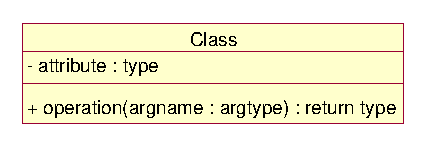
\includegraphics{umlClassIcon.eps}
        \caption{The class icon in UML.}
        \label{fig:umlClassIcon}
    \end{center}
\end{figure}
This icon is shown in Fig.~\ref{fig:umlClassIcon}.  A class icon is
simply a rectangle divided into three compartments. The topmost
compartment contains the name of the class. The middle compartment
contains a list of attributes (member variables), and the bottom
compartment contains a list of operations (member functions).  In many
diagrams, the bottom two compartments are omitted. Even when they are
present, they typically do not show every attribute and operations.
The goal is to show only those attributes and operations that are
useful for the particular diagram.  There is typically never a need to
show every attribute and operation of a class on any diagram.
\begin{figure}[htb]
    \begin{center}
        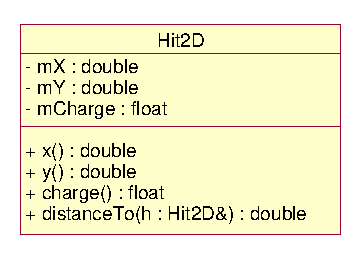
\includegraphics{umlClass.eps}
        \caption{Hit2D class. Attributes and operations are shown.}
        \label{fig:umlClass}
    \end{center}
\end{figure}
Fig.~\ref{fig:umlClass} shows a typical UML description of a class
that represents a Hit (here fictitious Hit2D).  Notice that each
member variable is followed by a colon and by the type of the
variable. If the type is redundant, or otherwise unnecessary, it can
be omitted. Notice also that the return values follow the member
functions in a similar fashion. Again, these can be omitted. Finally,
notice that the member function arguments also have a name and type.
Again one can omit the name or the arguments altogether.

At the beginning of each attribute and operations the visibility of
the class is indicated through a simple tag. UML provides three tags:
\begin{description}
\item[+] public
\item[\#] protected
\item[--] private
\end{description}
These abbreviations match exactly the three levels of visibility
provided in C++. The class shown in Fig.~\ref{fig:umlClass} is then
translated into C++ code as follows:

{\footnotesize
\begin{verbatim}
class Hit2D {
public:
    double x();
    double y();
    double distanceTo(Hit2D& h);
private:
    double mX, mY;
    float  mCharge;
};
\end{verbatim}
}%\footnotesize

\subsection{Composition Relationships}

Each instance of type Hit usually contains an instance of type
Position. One also says the Hit \emph{has} a Position. This is a
relationship known as composition. It can be depicted in UML using a
class relationship.  Fig.~\ref{fig:umlComposition} shows the
\emph{composition} relationship.
\begin{figure}[htb]
    \begin{center}
        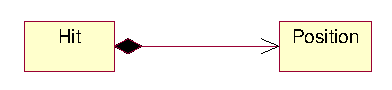
\includegraphics{umlComposition.eps}
        \caption{Class Hit has a Position.}
        \label{fig:umlComposition}
    \end{center}
\end{figure}
The black diamond represents composition. It is placed on the Hit
class because it is the Hit that is composed of (or has) a Position.
The arrowhead on the other end of the relationship denotes that the
relationship is navigable in only one direction. That is, Position
does not know about Hit. In UML relationships are presumed to be
bidirectional unless the arrowhead is present to restrict them.
Composition relationships are a strong form of containment or
aggregation. Aggregation is a whole/part relationship. In this case,
Hit is the whole, and Position is part of Hit. However, composition is
more than just aggregation. Composition also indicates that the
lifetime of Position is dependent upon Hit. This means that if Hit is
destroyed, Position will be destroyed with it.  In C++ we would
represent this as:

{\footnotesize
\begin{verbatim}
class Hit {
     Position mPos;
};
\end{verbatim}
}%\footnotesize

In this case we have represented the composition relationship as a
member variable. We could also have used a pointer so long as the
destructor of Hit deleted the pointer.  A more realistic example can
be found in \StEvent. There the \name{StHit} class has a member of
type \name{StThreeVector} which represents a position.

\subsection{Inheritance}

The inheritance relationship in UML is depicted by a triangular
arrowhead which points to the base class. One or more lines proceed
from the base of the arrowhead connecting it to the derived classes.
\begin{figure}[htb]
    \begin{center}
        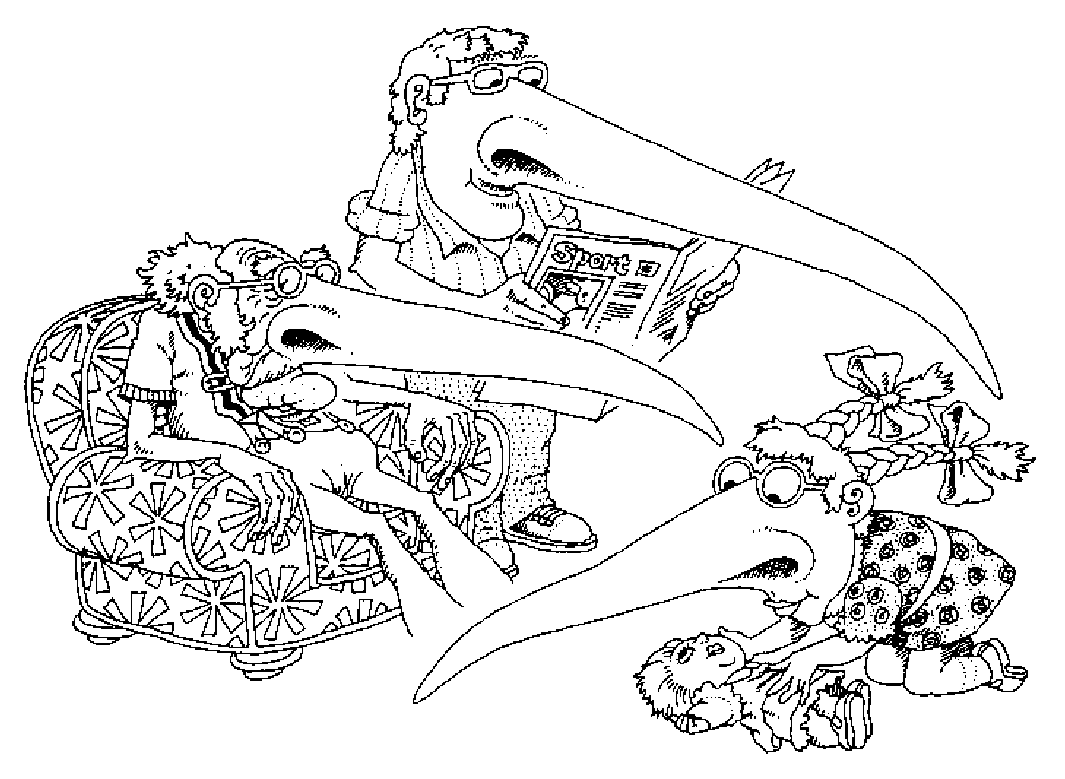
\includegraphics[width=0.7\textwidth]{cartoon6.eps}
        \caption{A subclass may inherit the structure and behaviour
            of its superclass.}
    \end{center}
\end{figure}
\begin{figure}[htb]
    \begin{center}
        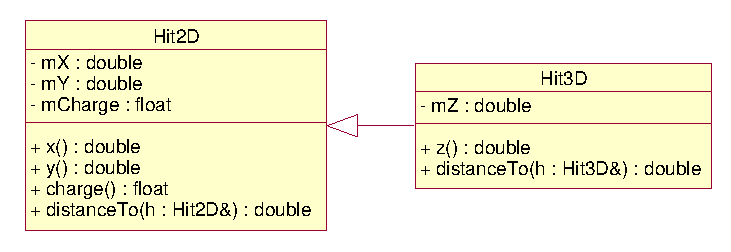
\includegraphics{umlInheritance.eps}
        \caption{Inheritance.}
        \label{fig:umlInheritance}
    \end{center}
\end{figure}

Fig.~\ref{fig:umlInheritance} shows the form of the \emph{inheritance}
relationship.  In this diagram we see that Hit3D is derived from
Hit2D.  If the name of a class would be shown in italics, it would
indicate that the class is an abstract class.  Note also that
operations shown in italics indicate that they are pure virtual.  The
corresponding C++ code for the Hit3D class from
Fig.~\ref{fig:umlInheritance} would look like:

{\footnotesize
\begin{verbatim}
class Hit3D : public Hit2D {
public:
    double z();
    double distanceTo(Hit3D& h);
private:
    double mZ;
};
\end{verbatim}
}%\footnotesize

\subsection{Aggregation and Association}

The weak form of aggregation is denoted with an open diamond. This
relationship denotes that the aggregate class (the class with the
white diamond touching it) is in some way the "whole", and the other
class in the relationship is somehow "part" of that whole.
Fig.~\ref{fig:umlAggregation} shows an \emph{aggregation}
relationship.
\begin{figure}[htb]
    \begin{center}
        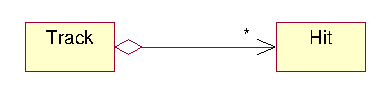
\includegraphics{umlAggregation.eps}
        \caption{Aggregation.}
        \label{fig:umlAggregation}
    \end{center}
\end{figure}
In this case, the Track class contains many Hit instances. In UML the
ends of a relationship are referred to as its "roles''. Notice that
the role at the Hit end of the aggregation is marked with a "$*$".
This indicates that the Track contains many Hit instances.  The
following Listing shows how Fig.~\ref{fig:umlAggregation} might be
implemented in C++ as:

{\footnotesize
\begin{verbatim}
class Track {
public:
    // ...
private:
    vector<Hit*> mHits;
};
\end{verbatim}
}%\footnotesize

There are other forms of containment that do not have whole/part
implications. For example, each \name{Vertex} refers back to its
parent Track. This is not aggregation since it is not reasonable to
consider a parent Track to be part of a child Vertex. We use the
\emph{association} relationship to depict this.

\begin{figure}[htb]
    \begin{center}
        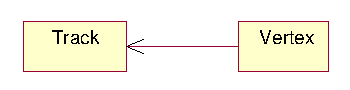
\includegraphics{umlAssociation.eps}
        \caption{Association.}
        \label{fig:umlAssociation}
    \end{center}
\end{figure}

Fig.~\ref{fig:umlAssociation} shows how we draw an association.  An
association is nothing but a line drawn between the participating
classes. In Fig.~\ref{fig:umlAssociation} the association has an
arrowhead to denote that Track does not necessarily know anything
about Vertex. This relationship will almost certainly be implemented
with a pointer of some kind.

What is the difference between an aggregation and an association?
Aggregation denotes whole/part relationships whereas associations do
not. However, there is not likely to be much difference in the way
that the two relationships are implemented.  That is, it would be very
difficult to look at the code and determine whether a particular
relationship ought to be aggregation or association.  Aggregation and
Association both correspond to the \emph{has-by-reference}
relationship.

\subsection{Dependency}

Sometimes the relationship between a two classes is very weak. They
are not implemented with member variables at all. Rather they might be
implemented as member function arguments.

Consider, for example, the fit function of a TrackFitter class.
Suppose that this function takes an argument of type CalibrartionDB
since it requires information from it (e.g. if the magnetic field was
on or off) in order to perform the fit.
\begin{figure}[htb]
    \begin{center}
        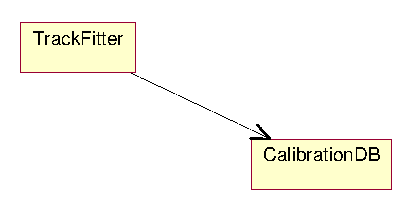
\includegraphics{umlDependency.eps}
        \caption{Dependency.}
        \label{fig:umlDependency}
    \end{center}
\end{figure}
Fig.~\ref{fig:umlDependency} shows a dashed arrow between the
TrackFitter class and the CalibrartionDB class. This is the
\emph{dependency} relationship. This is often called a \emph{using}
relationship.  This relationship simply means that TrackFitter somehow
depends upon CalibrartionDB. In C++ this almost always results in a
\#include:

{\footnotesize
\begin{verbatim}
#include "CalibrartionDB.hh"
class TrackFitter {
public:
    // ...
    void fit(CalibrartionDB &db);
private:
    // ...
};
\end{verbatim}
}%\footnotesize

%%%%%%%%%%%%%%%%%%%%%%%%%%%%%%%%%%%%%%%%%%%%%%%%%%%%%%%%%%%%%%%%%%%%
%
% The End
%
%%%%%%%%%%%%%%%%%%%%%%%%%%%%%%%%%%%%%%%%%%%%%%%%%%%%%%%%%%%%%%%%%%%%

\printindex

\end{document}
\bye

% The text following after this line is not included into the text
%
%  Template for reference section
%

%%%%%%%%%%%%%%%%%%%%%%%%%%%%%%%%%%%%%%%%%%%%%%%%%%%%%%%%%%%%%%%%%%%%
%
%    Reference: className
%
%%%%%%%%%%%%%%%%%%%%%%%%%%%%%%%%%%%%%%%%%%%%%%%%%%%%%%%%%%%%%%%%%%%%
\subsection{className}
\index{className|textbf}
\label{sec:className}
\begin{Entry}
\item[Summary]

\item[Synopsis]
    \verb+#include "className.hh"+\\
    \verb+class className;+\\

\item[Description]

\item[Persistence]
    None

\item[Related Classes]

\item[Public\\ Constructors]

\item[Public Member\\ Functions]

\item[Public Member\\ Operators]

\item[Public Functions]

\item[Public Operators]

\item[Examples]
{\footnotesize
\begin{verbatim}
//
//  What the example does
//

\end{verbatim}
}%footnotesize
\end{Entry}
\bye